\documentclass[12pt]{report}
\usepackage[utf8]{inputenc}
\usepackage{a4wide}
\usepackage[Lenny]{fncychap}
\usepackage[italic]{hepnames}
\usepackage{graphicx}
\graphicspath{{images/}}
\usepackage{fancyhdr}
\pagestyle{fancy}
\fancyhf{}
\lhead{\bfseries\nouppercase\leftmark}
\cfoot{\thepage}
\newcommand{\q}[1]{``#1''}
\usepackage{multirow}
\usepackage{gensymb}
\usepackage{array}
\usepackage[resetlabels,labeled]{multibib}
\usepackage{caption}
\usepackage{subcaption}
\usepackage{amsmath}
\usepackage{wrapfig}
\usepackage{sidecap}
\title{Thesis Title}
\author{Meena Nadeem}
\date{Day Month Year}

\begin{document}

\begin{titlepage}
    \begin{center}
        \vspace*{1cm}
            
        \Huge
        \textbf{Measurement of signal strength modifier $\mu$ of the Higgs boson decaying in four-lepton final state in pp collisions at $\sqrt{s}$ = 13 TeV}
            
        \vspace{0.5cm}
        \LARGE
        By
            
        \vspace{1cm}
            
        \textbf{Meena Nadeem}
            
        \vfill
            
       
        \vspace{0.8cm}
            
        
\includegraphics[width=0.5\textwidth]{images/QAU-PIC.jpg}
            
        \Large
        Department of Physics\\
        Quaid-I-Azam Unversity\\
        Islamabad, Pakistan\\
            
    \end{center}
\end{titlepage}





\chapter*{Dedication}
\vskip 0.2in
I am obliged to conduct my master program as a student of Quaid-I-Azam university, Islamabad. There were many experienced physicists around me and I could get their help and advice whenever I wanted. I was able to extend and develop my knowledge about high energy physics by the assistance from these people.
\newline
First of all I wish to express my sincere appreciation to my supervisor, Dr. Shamona Fawad Qazi, she convincingly guided and encouraged me to be professional even when things got difficult. Without her persistent help, the goal of this research work could not have been concluded.
\newline
I am extremely thankful to my instructor and co-supervisor, Dr. M. Bilal Kiani. He has always been supportive during the entire period of my master research work. Dr. Kiani has provided me with valuable discussions and advice. He introduced me to CMSSW, CMS offline software and how it operates, new to a novice like me. He has spent enormous time in teaching me and discussing data analysis with me.
\newline
The physical and technical contribution of ‘National Center for Physics (NCP), Islamabad’ is truly appreciated. Without their support and funding, my research work could not have reached its goal.
\newline
Now I have to thank my family, especially my parents. They were always very supportive and foundation behind this strenuous period.
\newline 
I am sincerely thankful to my senior Iqra and junior Sumaira. A constant support in this period.
\newline
I am also thankful to my research mates Jamshed, Sajid and Sunila for their insights and inputs whenever i got stuck on a problem.
\newline
There are still many more people I have to thank Afroze, Aiman, Arfa, Azkah, Esha, Hurriyat, Rafia, Mariyam (for the headphones), Mishal, Sana and Sephora. I am grateful to all of those colleagues who helped me directly or indirectly, in any way during this period.
\thispagestyle{empty}

\chapter*{Abstract}
\hspace{5mm}The detection of a new particle with mass approximately 125 GeV and properties consistent with Higgs Boson affirmed the Standard Model (SM) of particle physics, a theory which till now explained three of the four known fundamental forces. The Standard Model of particle physics was able to quite accurately match the theoretical calculations to the corresponding experimental checks. However it was still undiscovered; how $W$ and $Z$ boson attained mass while the photon remained massless, how to keep local gauge symmetry intact and validating the theory at TeV energy scale or, similarly, at smaller distances.\\

Hence, LHC was built by the scientific community in 2008, the main purpose of which was to investigate the so called ``God particle", Higgs boson, as it gives mass to all matter. Higgs boson was discovered in 2012 \cite{<ob1>,<ob2>} and after that studies have been going on to further understand its nature. In this thesis, we will model the Higgs signal around mass $m_H$=125 GeV for five main production modes collected from its decay through the ($H \rightarrow ZZ^* \rightarrow 4l$) ``Golden Channel'', where $l=\mu,e$, using Run II data accumulated in the CMS detector. We will use statistical functions to model and fit the data for the Higgs signal and irreducible background. It will list the yields calculated for the 2016, 2017 and 2018 Monte Carlo (MC) data samples. Lastly, the signal strength modifier for Higgs boson will be measured for whole Run II data at centre-of-mass energy $\sqrt{s}$=13 TeV.


\thispagestyle{empty}

\tableofcontents


\chapter{Introduction to Particle Physics}
The Standard Model (SM) of particle physics, a gauge quantum field theory was developed to describe three fundamental forces in the universe: strong force, weak force and the electromagnetic force and simultaneously, classifies elementary particles.\\
To explain how the gauge bosons acquired mass in SM, a complex scalar doublet field which self-interacted and allowed spontaneous electroweak symmetry breaking (EWSB), was introduced, with the inclusion of a new particle known as \q{Higgs Boson}. The following chapter will give an overview of the theory of Standard Model of particle physics, the production and decay modes of Higgs along with a brief description of the golden channel. Finally, the chronicle searches by LHC experiments to find Higgs boson.

\section{Particle Physics}
\subsection{Building Blocks of Particle Physics}
Elementary particles are the basic units of Standard Model. The elementary particles are split into two spin families: fermions (spin = $\frac{1}{2}$) and bosons (spin = 1). The Standard Model elementary particles are matter particles (leptons and  quarks), the force carriers ($W, Z,$ \Pphoton, \Pgluon) and the Higgs boson. Leptons and quarks are divided into three generations as they are spin $\frac{1}{2}$ fermions. The particles in each generation have different flavour and mass. Generation 1 contains the lightest and the most stable particles while the heaviest and most unstable one are classified in the second and the third generations. The fermion's classification is shown in Table.\ref{tab:ep} \cite{<PDG>}. The bar above the symbol of the particle represents anti-particle with an opposite quantum number.\\ 
Leptons exist as free particles in nature and interact by electroweak (EWK) interaction, while quarks in hadrons interact by means of both strong and EWK interactions. A pair of quark with an anti-quark forms a meson which is a bosonic hadron while 3 (anti)quarks form (anti)baryon which is a fermionic hadron.\\
Standard model force carriers consist of; massless photons (\Pphoton) which mediates the electromagnetic (EM) force, three gauge bosons (\PZ, \PWpm) which mediate the weak force and 8 massless gluons (\Pgluon) are conducive for the strong force. Higgs boson (\PHiggs) was the last discovered, a heavy scalar particle which mediates the Higgs field. Table.\ref{tab:boson}  \cite{<PDG>} shows some properties of force mediators.
\begin{table}[]
    \centering
    \begin{tabular}{|c|l|l|l|l|l|l|}
    \hline
         Generation & Flavour& Symbol & Family & Mass(GeV) & Charge(e) & Interaction\\
     \hline 
     \hline
         \multirow{2}{*}{I} & electron &\Pe & lepton & 0.000511 & -1 & EM,Weak \\ 
         & \Pe neutrino &  \Pnue &lepton& $<1.18^{-8}$ & 0 & Weak\\ 
         \hline
         \multirow{2}{*}{II} & muon & \Pmu  & lepton & 0.106 & -1 & EM, Weak\\
         & \Pmu neutrino& \Pnum & lepton & $<0.002$ & 0 & Weak\\
         \hline 
         \multirow{2}{*}{III} & tau & \Ptau & lepton& 1.777 & -1 & EM, Weak\\
         & \Ptau neutrino & \Pnut & lepton & $<0.02$ & 0 & Weak\\
         \hline 
         \multirow{2}{*}{I} & up &\Pup & quark & 0.002 & $ \frac {2}{3}$ & All \\
         & down & \Pdown & quark &0.005 & $-\frac{1}{3}$ & All \\
         \hline
         \multirow{2}{*}{II} & charm & \Pcharm & quark & 1.275 & $ \frac {2}{3}$ & All  \\
         & strange &\Pstrange & quark & 0.095 & $-\frac{1}{3}$ & All\\
         \hline 
         \multirow{2}{*}{III} &top & \Ptop & quark & 173 & $ \frac {2}{3}$ & All\\
         & bottom & \Pbottom & quark &4.18 & $-\frac{1}{3}$ & All\\
         \hline
    \end{tabular}
    \caption{Distribution of Fermions}
    \label{tab:ep}
\end{table}

\begin{table}[h]
\centering
\begin{tabular}{| l | l | l | l | l| l|}
\hline
\multicolumn{6}{|c|}{FORCE MEDIATORS} \\
\hline
\hline
Name & Symbol & Spin & Charge(e) & Mass[GeV] & Mediates \\
\hline
Photon & \Pphoton & 1 & 0 & 0 & EM \\
$\PWpm$ Boson & \PWpm & 1 & $\pm1$ & 80.4 & Weak \\
$Z^0$ Boson& \PZzero & 1 & 0 & 91.2 & Weak \\
gluons & \Pgluon & 1 & 0 & 0 & Strong \\
Higgs boson & \PHiggs & 0 & 0 & 125 & Higgs Field\\
graviton & $G$ & 2 & 0 & 0 & Gravitation \\
\hline
\end{tabular}
\caption{Distribution of Force Carriers}
\label{tab:boson}
\end{table}

\subsection{Quantum Field Theory of Particle Physics}
All building blocks are quantum fields in Standard Model which define the whole space time. The fields are given below;
\begin{itemize}
    \item Field of fermions for matter, $\Ppsi$.
    \item Fields of EWK boson, $W_1, W_2, W_3$ and B;
    \item Fields of gluons $G_a$,
    \item Field of Higgs, $\Pphi$.
\end{itemize}

The fundamental fields and fluctuations in quantum states are determined with Lagrangian density $\mathcal{L}$. The Standard Model does not vary under local gauge symmetry, where parameter conversion is a function of points in space that the particular field spans. The gauge group describing the Standard Model is $SU(3)_C \times SU(2)_L \times U(1)_Y$ where the index $C$ represents colour, $L$ represents left-handed and $Y$ is for hypercharge, respectively. The $SU(3)_C$ acts on $G_a$, $SU(2)_L$ acts on $W$ and $\Pphi$, and $U(1)_Y$ acts on $B$ and $\Pphi$.\\
The next section will give an overview of the conventions used to construct strong interaction through local gauge symmetry, based on Quantum Chromodynamics (QCD). Glashow-Weinberg-Salam \cite{<gws>} used an identical formalism for EWK theory which unifies electromagnetic and weak interactions, built upon weak hypercharge and weak iso-spin group represented by $U(1)_Y \times SU(2)_L$.\\

\textbf{QUANTUM COLOR THEORY}\\

Quantum Chromodynamics (QCD) expresses the interaction amidst gluons and quarks, built upon $SU(3)_C$ symmetry group. Quantum number is the colour that can take three possibilities: green, red and blue. $SU(3)_C$ symmetry group is a non-commutative group which consists of 8 Gell-Mann matrices $\frac{\lambda_a}{2}$, $a$=generator number, to the corresponding 8 generators. The Dirac Lagrangian is defined as:
\begin{equation}
    \mathcal{L}_{QCD}=\Paq_{f}(i\Pgg^{\mu}\partial_\mu-m)\Pquark_f.
\end{equation}
As the quark fields have linear transformation under the local gauge symmetry, the Lagrangian remains constant:
\begin{equation}
    \Pquark_f(x) \rightarrow e^{-i\alpha_a (x) \frac{\lambda_a}{2}} \Pquark_f (x),
\end{equation}
whereas the Minkowski space derivatives are not linearly transformed. A covariant derivative is reinstated in place of $\partial_\mu$:
\begin{equation}
    D_\mu=\partial_\mu + i g_s \frac{\lambda_a}{2}G^a_\mu,
\end{equation}
where $g_s$, a linking constant and 8 gauge vector fields $G^a_\mu$ analogous to 8 gluons, are transformed as:
\begin{equation}
    G^a_\mu=G^a_\mu + \alpha^b (x) f^{abc}G^c_\mu + \frac{1}{g_s} \partial_\mu \alpha^a (x),
\end{equation}
where the structure constants are denoted with $f^{abc}$. Each gauge field corresponds to a specific generator, given as force mediator in a Lagrangian. Ultimately, QCD Lagrangian with gauge invariance is defined as:
\begin{equation}
    \mathcal{L}_{QCD}=\Paq_{f}(i\Pgg^{\mu}\partial_\mu-m)\Pquark_f - g_s \Paq_f \Pgg^\mu \frac{\lambda_a}{2} \Pquark_f G^a_\mu - \frac{1}{4} G^{\mu\Pnu}_a G^a_{\mu\Pnu},
\end{equation}
by summing over all gauge fields.\\
First term in Eq.1.5 represents free Dirac Lagrangian, next term controls the interaction in between gluon fields and quark, and interactions in between gluon fields are shown by the last two trilinear and quadriliniear terms.\\

\textbf{ELECTROWEAK THEORY}\\

This is constructed by the symmetry group $SU(2)_L \times U(1)_Y$ and describes the interaction among four gauge bosons and leptons. The quantum numbers are hypercharge (Y) and weak iso-spin $(I_3)$, interrelated by the equation $Q=I_3 + \frac{Y}{2}$, where $Q$ is the electric charge. Major contrast between QCD theory and electroweak theory is the difference in interaction amongst opposite chirality fermions.\\
Singlets are denoted as $\Ppsi_R$ and $\Ppsi^{\prime}_R$ and $SU(2)_L$ doublets as $L=\binom{\Ppsi_L}{\Ppsi^{\prime}_{L}}$, and , now the free electroweak Lagrangian becomes:
\begin{equation}
    \mathcal{L}_{EW}=\bar{L}i\Pgg^{\mu}\partial_{\mu}L + \bar{\Ppsi}^\prime_R i \Pgg^{\mu}\partial_{\mu}\Ppsi^\prime_R
\end{equation}
Like before, under the local gauge theory we linearly convert singlets and doublets:
\begin{equation}
    L \rightarrow e^{-i\alpha_i (x) \frac{\sigma_i}{2}-i\beta(x)\frac{Y}{2}} L, \hspace{4mm} \Ppsi^\prime_R \rightarrow e^{-i\beta(x)\frac{Y}{2}}\Ppsi^\prime_R
\end{equation}
here the Pauli matrices are $\frac{\sigma_i}{2}$ which serve as $SU(2)_L$ generators. We replace partial derivatives with corresponding covariant derivatives as we did for QCD:
\begin{equation}
\begin{aligned}
    L:  D_\mu = \partial_\mu + i g_w \frac{\sigma_i}{2} W^i_\mu + ig\frac{Y}{2} B_\mu,\\
    \Ppsi_R,\Ppsi^\prime_R: \hspace{10mm} D_\mu=\partial_\mu +ig\frac{Y}{2}B_\mu,
\end{aligned}
\label{eqn:sp}
\end{equation}
here $g_w$ and $g$ are coupling constants and 3+1 gauge fields are introduced. Transformation of gauge fields can be seen as:
\begin{equation}
\begin{aligned}
    W^i_\mu \rightarrow W^i_\mu + \alpha^j(x)\epsilon^{ijk}W^k_\mu + \frac{1}{g_w}\partial_\mu \alpha^i(x),\\
    B_\mu \rightarrow B_\mu + \frac{1}{g}\partial_\mu \beta(x),
\end{aligned}
\end{equation}
here $\epsilon^{ijk}$ are the group structure constants. Linear combinations of the bosonic fields ($W^i_\mu$, $B_\mu$, $\PWpm_\mu$, $Z_\mu$) and photonic fields $A_\mu$ can be written as:
\begin{equation}
    \begin{aligned}
    \PWpm_\mu = \frac{1}{\sqrt{2}}(W^1_\mu \mp iW^2_\mu),\\
    Z_\mu = W^3_\mu cos\theta_w - B_\mu cos \theta_w,\\
    A_\mu = W^3_\mu sin \theta_w + B_\mu sin \theta_w
    \end{aligned}
\end{equation}
$\theta_w$ (weak mixing angle) comes from sin$\theta_w=\frac{g}{\sqrt{g_w^2+g^2}}$. To get the expression for the full electroweak langrangian we replace covariant derivative with partial one:
\begin{equation}
\begin{aligned}
    \mathcal{L}_{EW}=\bar{L}i\Pgg^\mu\partial_\mu L + \bar{\Ppsi}^\prime_R i \Ppsi^\mu \partial_\mu \Ppsi^\prime_R - g_w\bar{L}\Ppsi_\mu\frac{\sigma_i}{2}LW^i_\mu - g\bar{L}\Ppsi^\mu\frac{Y}{2}LB_\mu \\- g \bar{\Ppsi}^\prime_R\Pgg^\mu\frac{Y}{2}\Ppsi^\prime_R B_\mu - \frac{1}{4} W_i^{\mu\Pnu}W^i_{\mu\Pnu} - \frac{1}{4} B^{\mu\Pnu} B_{\mu\Pnu},
\end{aligned}
\end{equation}
summing over singlets and doublets. Like in Eq.1.6, free Dirac Lagrangian is shown in first two  terms, third to fifth are interactions shown by the Feynman rules between force carriers ($Z$,\PWpm,\Pgg) and fermions of the electroweak interactions. The leftover terms describes the gauge bosons participating in electroweak interactions. \\

\textbf{ELECTROWEAK SYMMETRY BREAKING AND BEH MECHANISM}\\

QCD and EW theory predict interaction at an unprecedented scale assuming elementary particles are massless and become unperturbed at TeV scale. A mass term will violate the Lagrangian invariance under gauge symmetry and here spontaneous symmetry breaking (SSB) is the solution. This solution most popularly called the Brout-Englert-Higgs (BEH) mechanism, published in three autonomous papers, by Brout and Englert \cite{<brout>} , Higgs \cite{<higgs>} and Kibble, Guralink and Hagen \cite{<guralnik>}.\\
The new field introduced by the BEH mechanism was symmetric under the Standard Model gauge transformations and broke the electroweak symmetry by obtaining a non-zero expectation number within the vacuum state. These properties describe a field with a $SU(2)_L$, a scalar complex doublet fields:
\begin{equation}
    \Pphi = \binom{\Pphi^{+}}{\Pphi^{-}} = \frac{1}{\sqrt{2}} \binom{\Pphi^{1}+i\Pphi^{2}}{\Pphi^{3}+i\Pphi^{4}}
\end{equation}
in SM Lagrangian the term which represents this is:
\begin{equation}
    \mathcal{L}_{Higgs}=(D_\mu \Pphi)^\dagger(D_\mu \Pphi) + V(\Pphi), 
\end{equation}
the covariant derivative $D_\mu$ comes from Eq.\ref{eqn:sp} and scalar field potential is depicted by V$(\Pphi)$:
\begin{equation}
    V(\Pphi)=\mu^2\Pphi^\dagger\Pphi + \lambda (\Pphi^\dagger\Pphi)^2,
\end{equation}
where $\lambda$ and $\mu^2$ are constants. The potential for a ground state is bounded underneath by $\lambda > 0$ and $\mu^2 < 0$ for the spontaneous symmetry breaking. These constants give ground states a number of non-zero values, in place of a trivial $\Pphi = 0$, written as:
\begin{equation}
    \Pphi^\dagger\Pphi= - \frac{\mu^2}{2\lambda}\equiv \frac {\Pnu^2}{2}
\end{equation}
A specific ground state which spontaneously breaks the $SU(2)_L \times U(1)_Y$ symmetry, where a electromagnetic subgroup $U(1)_{EM}$ remains symmetric in the vacuum. Three massless states correlating the corresponding broken $SU(2)_L$ generators emerge as was defined by the Goldstone theorem \cite{<goldstone>}. The scalar doublet can be parameterized as:
\begin{equation}
    \Pphi = e^{i\frac{\sigma_i}{2}\theta^i(x)}\binom{0}{\Pnu + \frac{h(x)}{\sqrt{2}}}
\end{equation}
here $\theta_i$ shows three massless fields; $h(x)$ shows a massive field and four scalar fields. Linear transformation of Higgs field in presence of local gauge symmetry is defined as:
\begin{equation}
    \Pphi= e^{-i\alpha_i(x)\frac{\sigma_i}{2}}\Pphi(x),
\end{equation}
here the $\theta^i$ fields are eradicated by $\alpha_i(x)=2\theta^i(x)$, where degrees of freedom of $\theta^i$ fields become \PWpm and $Z^0$ vector bosons longitudinal degrees of freedom.
Expanding Eq.1.18 by including the expression of covariant derivative, potential and the scalar fields, the full Higgs Langrangian is given as:
\begin{equation}
\begin{aligned}
    \mathcal{L}_{Higgs}=\frac{1}{2}\partial_\mu h \partial^\mu h +\mu^2 h^2 + \frac{g_w^2 \Pnu^2}{4} \PWminus_\mu \PWplus^\mu + \frac{g_w ^2 \Pnu^2}{8 cos \theta_w }Z_\mu Z^\mu +\frac{g_w^2 \Pnu_2}{2}h\PWminus_\mu \PWplus^\mu\\
    + \frac{g_w^2}{4}h^2 \PWminus_\mu \PWplus^\mu + \frac{g_w^2 \Pnu}{4cos^2 \theta_w}h^2 Z_\mu Z^\mu + \frac{\mu^2}{\Pnu} h^3 + \frac{\mu^2}{4\Pnu^2}h^4.
\end{aligned}
\end{equation}
Extension of this to Standard Model Lagrangian, grants mass to the Higgs boson ($m_H = \sqrt{2}|\mu|$),$\PWpm  (m_w= \frac{1}{2}g_w \Pnu)$ and $Z^0 (m_Z = \frac{g_w \Pnu}{2 cos \theta_w})$ bosons. This generates trilinear and quadrilinear terms for weak $VBH$ couplings and $HH$ couplings.\\
Also, Brout-Englert-Higgs mechanism adds extensions of gauge-invariant Yukawa terms to SM Lagrangian, that provide the fermions with their masses. The additional terms in the Lagrangian when the EWK symmetry breaks are given by:
\begin{equation}
    \mathcal{L}_{Yukawa}=\sum_f -m_f \bar{\Ppsi}\Ppsi \left(1+\frac{h}{\Pnu}\right) + \sum_{f\prime}  -m_{f^\prime} \bar{\Ppsi^\prime}\Ppsi^\prime \left(1+\frac{h}{\Pnu} \right)
\end{equation}
where first summation is over spin up fermions and the second summation is over spin down fermions. Besides the obligatory terms for fermions mass, the other terms suggest that the fermions and Higgs field interact, when couplings are proportional to their masses. There is a reduction in overall symmetry corresponding to the BEH mechanism, since there is no similarity in the three generations of matter.\\
The full SM Langrangian now becomes:
\begin{equation}
    \mathcal{L}_{SM}= \mathcal{L}_{QCD}+ \mathcal{L}_{EW}+ \mathcal{L}_{Higgs}+ \mathcal{L}_{Yukawa}.
\end{equation}

\section{Higgs Boson at Hadron Collider}
The motivation for building high energy accelerator machines operating at TeV scale was to find experimental proof for the existence of Higgs boson. In order to comprehend how the experiment was set up and the search proceeded, let us go through principal aspects of the production mechanisms and decay modes for identification of Higgs boson.\\ 
The progression of Standard Model proton-(anti)proton cross sections in accordance with centre of mass energy in pp colliders is exemplified in Fig.\ref{fig:x cross section}. The illustration shows benefits of raising the energy for Higgs boson will increase the cross section and event rate per second, the incentive behind the advancement of Large Hadron Collider (LHC).

\subsection{Production Mechanisms}
Higgs can be generated by different mechanisms in accordance with the SM theory. This section will describe the key production mechanisms which contributes to the Higgs boson production at pp colliders \cite{<HPL>,<PHT>}. The four main among all are indicated as lowest order Feynman's diagrams in Fig.\ref{fig:pm} and their cross section versus centre-of-mass energy distributions are shown in Fig.\ref{fig:Cross}.\\
\begin{figure}[h]
\centering
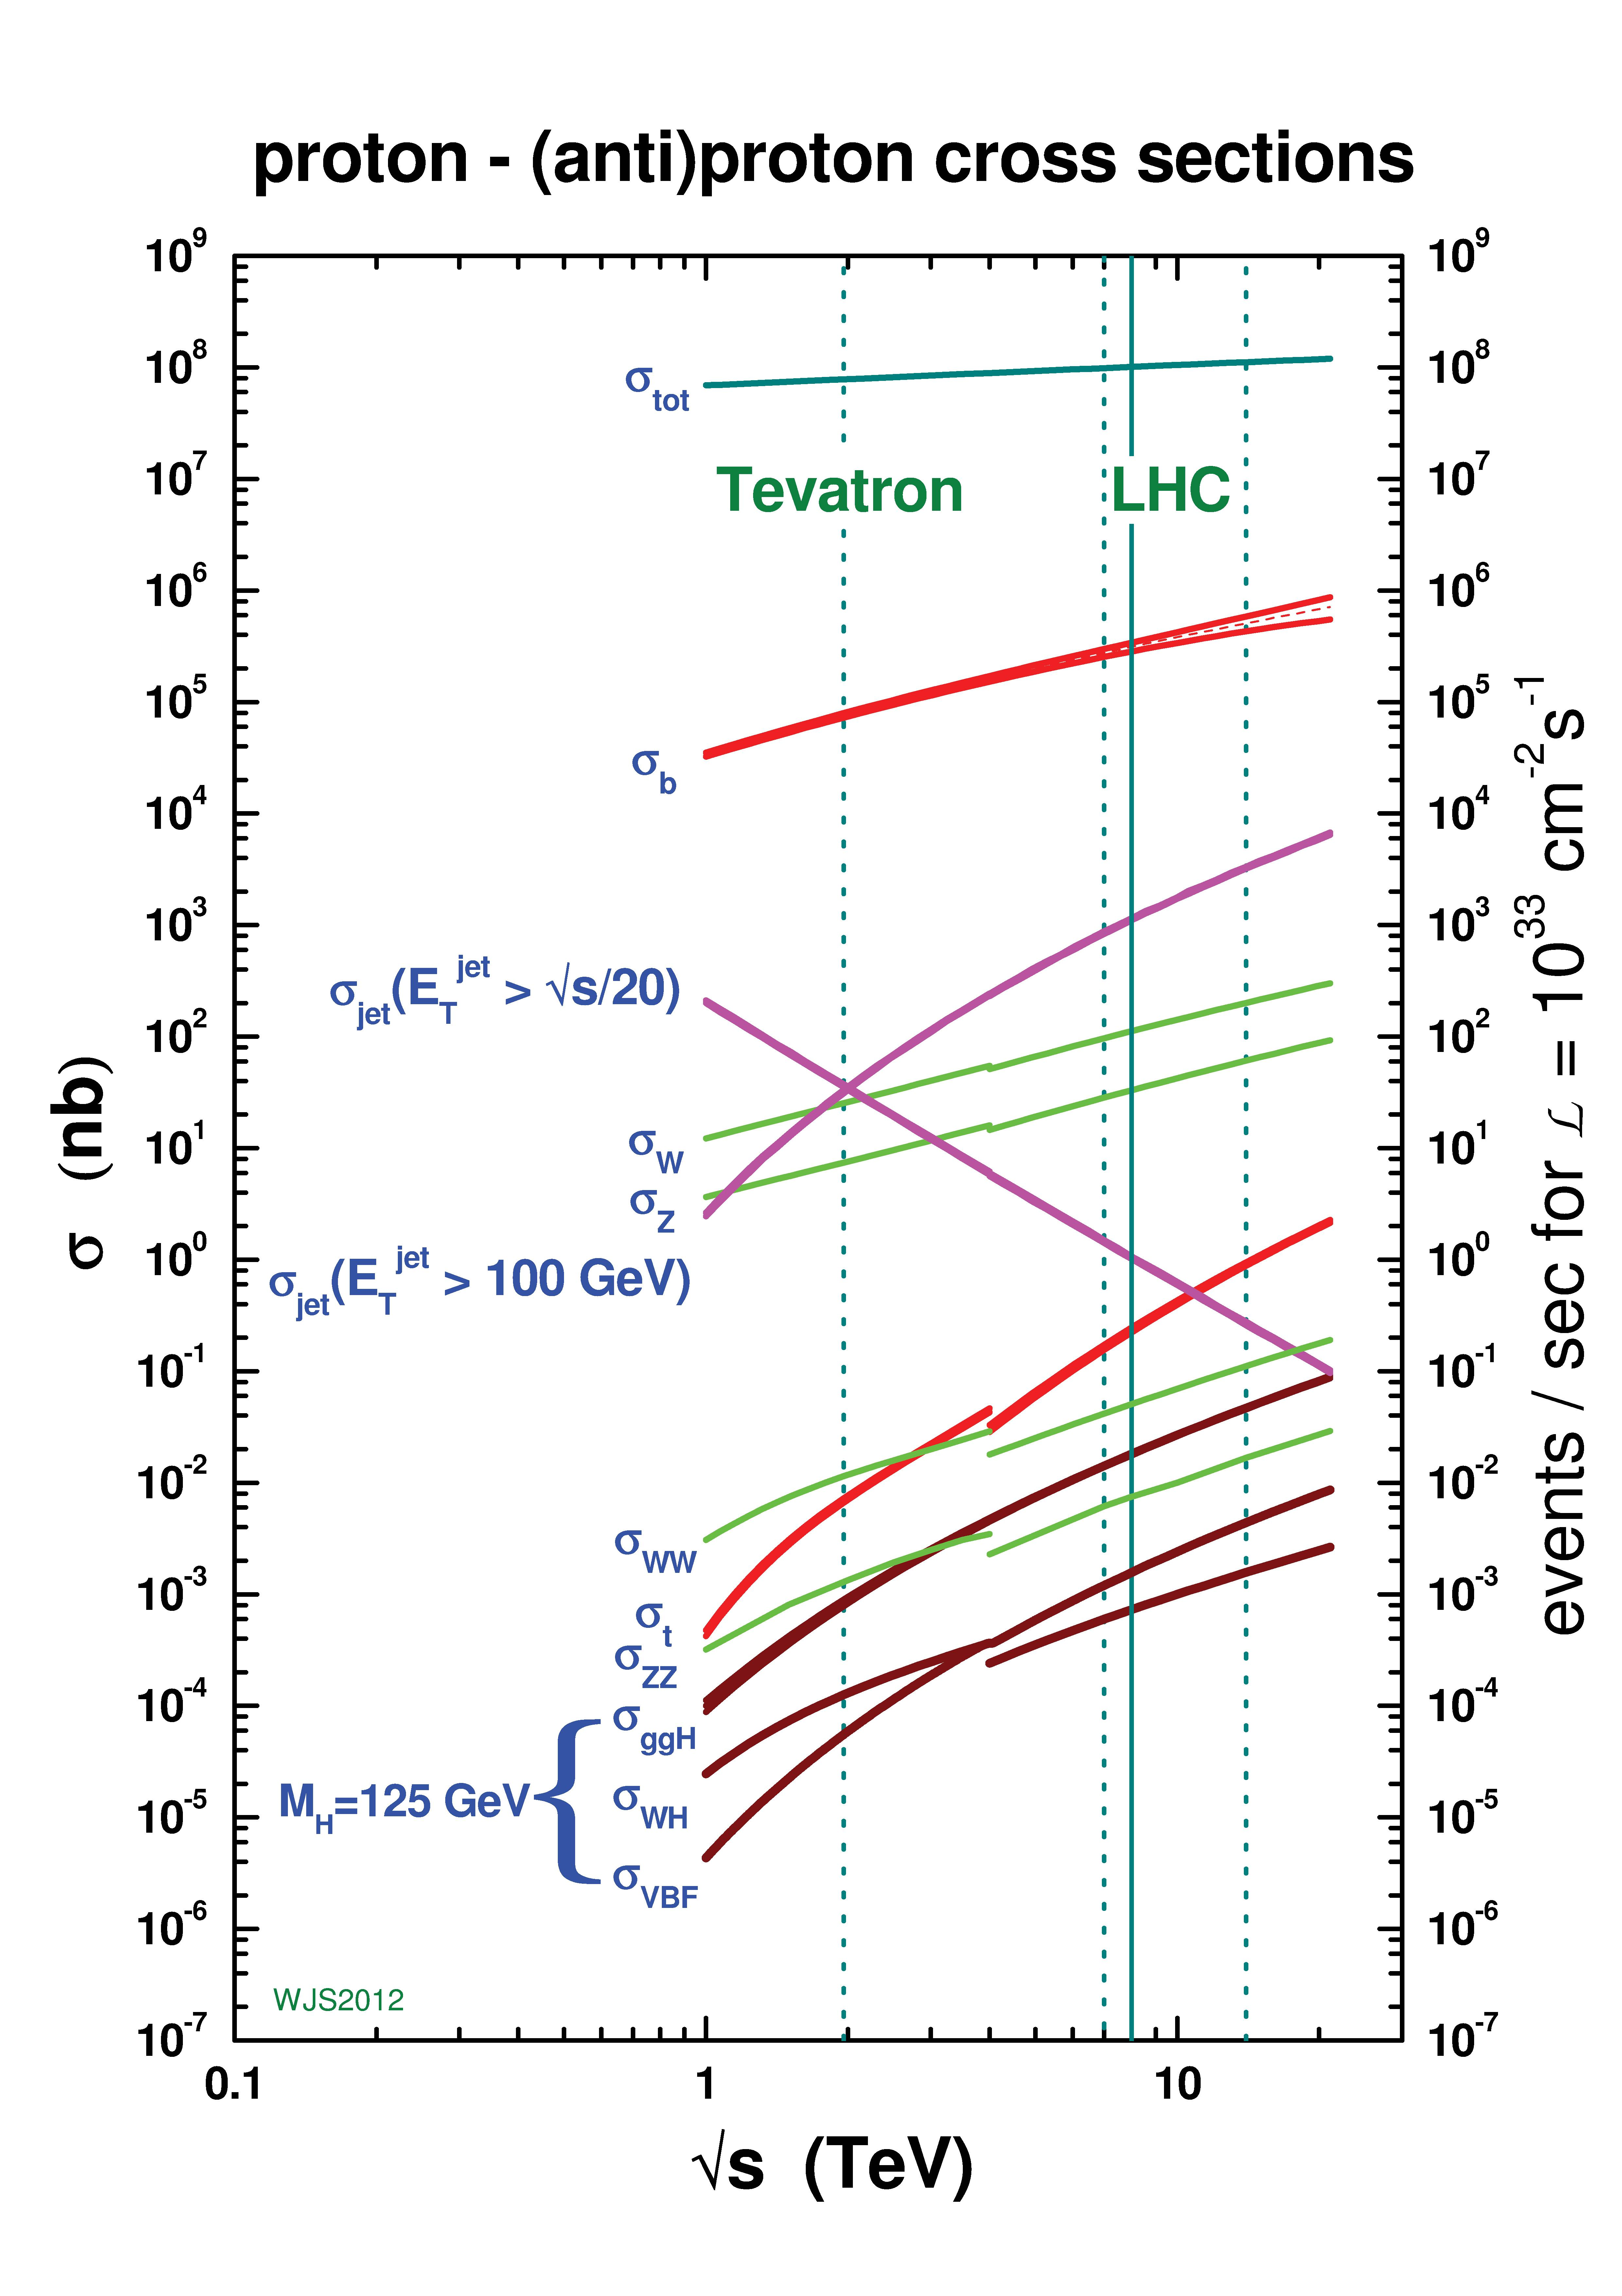
\includegraphics[scale=0.32]{images/cros.jpg}
\caption{Cross sections as a function of centre-of-mass energy \cite{<AQL>}.}
\label{fig:x cross section}
\end{figure}

\begin{figure}[h]
\centering
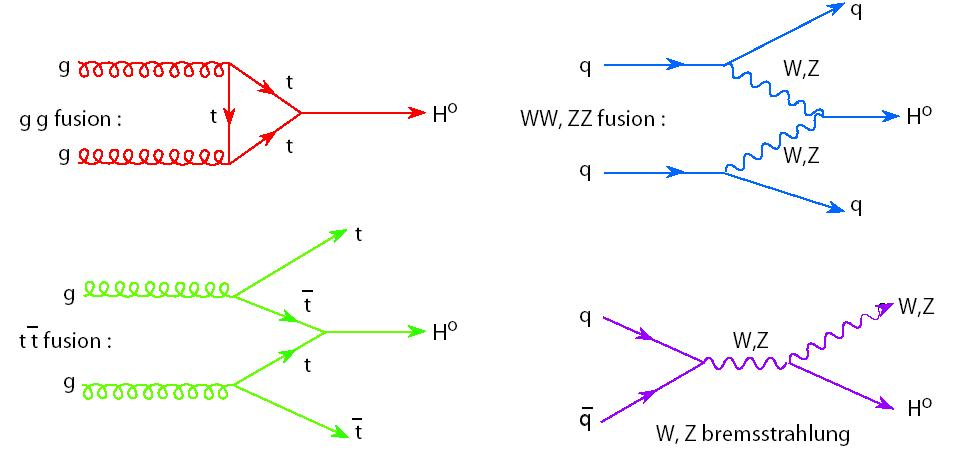
\includegraphics[scale=0.32]{images/Production Mechanism.jpg}
\caption{Feynman Diagrams For Prodcution of Higgs: (i)gluon fusion, (ii)vector boson fusion, (iii)$\Pqt\Paqt\PHiggs$ associated production, (iv)associated production with a vector boson \cite{<HPDC>}.}
\label{fig:pm}
\end{figure}

\vspace{5mm}
\textbf{GLUON FUSION} \\
In gluon-gluon fusion (ggH), two gluons merge by an intermediate quarks loop as demonstrated in Fig.\ref{fig:pm}(i), the main production mode with the largest cross section. It leads by more than one order of magnitude than the rest of the production modes as shown in Fig.\ref{fig:Cross}. This is due to the very high gluon luminosity when hadrons collide at TeV energies existing in the LHC. As top quark is the heaviest quark, its input is the largest to the loop amounting to $\sim$90\% and bottom quark accounts for other noticeable input $\sim$5-10\% out of the total cross section \cite{<PDG>}.\\
Quantum Chromodynamics corrections of higher orders are significant in this process, such as next-to-leading order(NLO) QCD corrections increase the cross sections by a factor of $\sim$2. High end computations are crucial as this thesis uses N3LO QCD and NLO EW computations \cite{<HPDGH>,<Handbook>}.

\vspace{5mm}
\textbf{VECTOR BOSON FUSION}\\
Vector boson fusion (VBF) is the next most prominent production mechanism having a cross section around an order of magnitude less than ggH as illustrated in Fig.\ref{fig:pm}(ii). This process takes place when a virtual \PZ or \PW boson is exchanged among two fermions, which fuse into Higgs boson. This mechanism has high invariant mass forward and backward energetic jets, which gives it a distinct experimental signature. The characteristic topology helps removing ggH production and Standard Model backgrounds provided by the two jets. The cross sections of leading order (LO) and NLO have \cite{<Handbook>} negligible uncertainties and QCD corrections of higher order are also very small.

\vspace{5mm}
\textbf{TOP QUARK ASSOCIATED PRODUCTION}\\
Associated production with a top and anti-top quark ($\Ptop\bar{\Ptop}$H) as displayed in Fig.\ref{fig:pm}(iii), is close to two orders of magnitude lower than ggH production and many times less than VBF production. It predominantly involves collision of two gluons, each of which decays into quark-antiquark pair. A quark and anti-quark from each of these pair, then fuse together into a Higgs boson. If the final state contains $\Ptop\bar{\Ptop}$ pair, a rare signature in experiments is seen which is used to measure this unique production mode. The QCD corrections are of the higher-order of around $\sim$1.2 and are compared at NLO EW + NLO QCD accuracy \cite{<Handbook>}.

\vspace{5mm}
\textbf{VECTOR BOSON ASSOCIATED PRODUCTION}\\
Vector boson associated production (also known as Higgs-Strahlung) also a prominent production mechanism which occurs about twice less frequently than vector boson fusion, is shown in Fig.\ref{fig:pm}(iv). In this process a pair of oppositely charged fermions fuse and generate a \PZ or \PW boson that subsequently produces Higgs boson.\\
In hardronic vector boson decays we see boosted jet pairs with fixed mass resembling vector boson's nominal mass. When there are leptonic decays, either missing transverse energy for $WH$ with one lepton or missing transverse energy for $ZH$ along with a pair of leptons are detected. The production mode has significant QCD corrections of higher order and thereby, computed with NLO EW + NNLO QCD accuracy \cite{<Handbook>}.


\begin{figure}
\centering
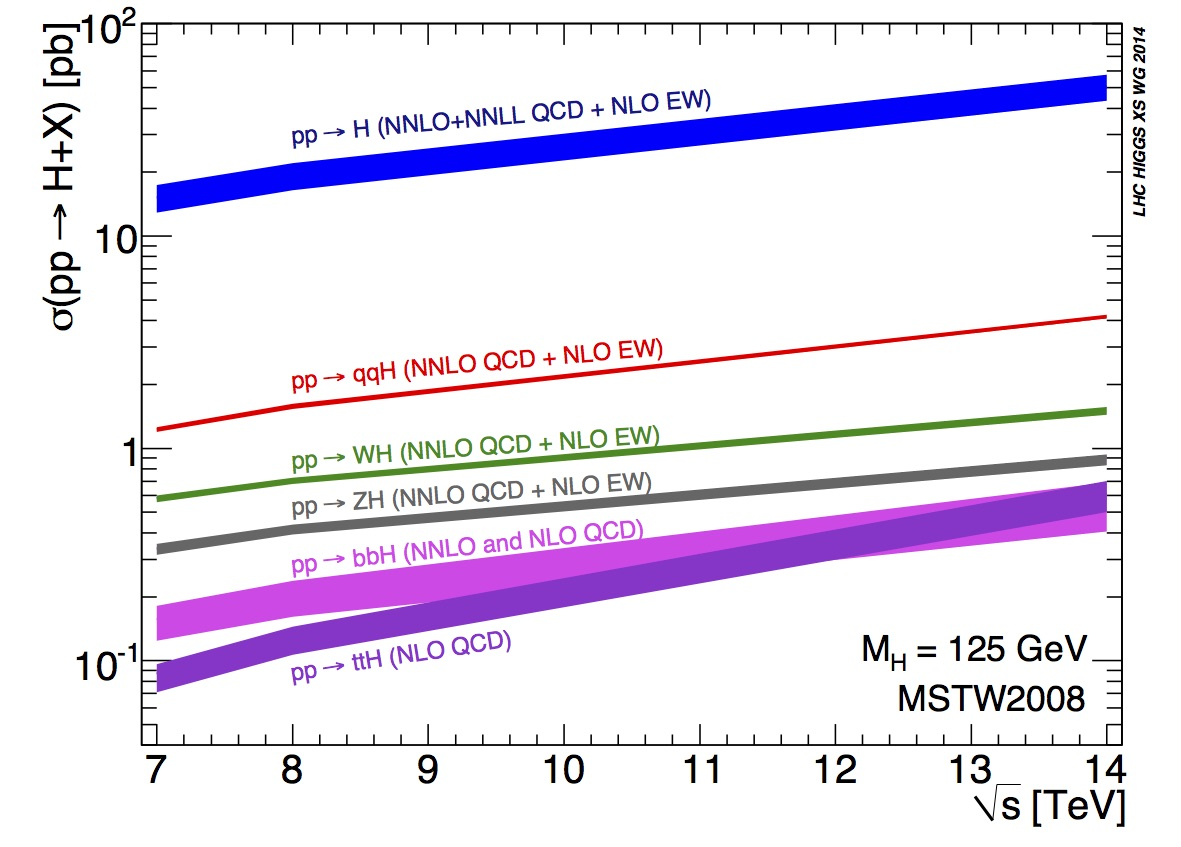
\includegraphics[scale=0.32]{images/Cross Sec.jpg}
\caption{Cross Section of Production Modes for $m_H$=125 GeV \cite{<Cross>}.}
\label{fig:Cross}
\end{figure}

\vspace{5mm}
\textbf{ADDITIONAL PRODUCTION MECHANISMS}\\
Bottom quarks associated production ($\Pqb\Paqb\PHiggs$) and production with top quark ($\Pqt\Pq\PHiggs$) are also taken into account during Higgs searches. The $\Pqb\Paqb\PHiggs$ and one of the $\Pqt\Paqt\PHiggs$ production channel have cross sections that are similar to each other, where as $\Pqt\Pq\PHiggs$ has an exclusive cross section one order of magnitude lower. Supplementary production channel of Higgs boson have even smaller cross section and hence, are not taken into consideration.

\subsection{Decay Mechanisms}
According to quantum mechanics, if a heavier particle can decay into lighter particles, then it eventually does. The probability of the decay is dependent on multiple factors, such as the strength of interactions, difference in mass, etc. SM sets parameters for these factors, except for the Higgs boson mass. For Higgs boson, the Standard Model anticipates a mean lifetime of $1.6\times10^{-22}$s at a mass of 125GeV \cite{<hb>}. The mean lifetime of decay products is used to detect the Higgs boson, as it is short-lived to reach the detector, on its own.\\
The branching ratios of the Higgs decay modes, predicted by the SM, depend on the Higgs mass value illustrated in Fig.\ref{fig:decaybr}. Since all the elementary particles interact with Higgs boson, it  can decay via many different processes. Higgs can decay through multiple processes, as it interacts with all elementary particles, such as decay to massless particles or through an intermediate virtual particles loop. Some of these are given in Table.\ref{tab:dec}.

\begin{table}[h]
\centering
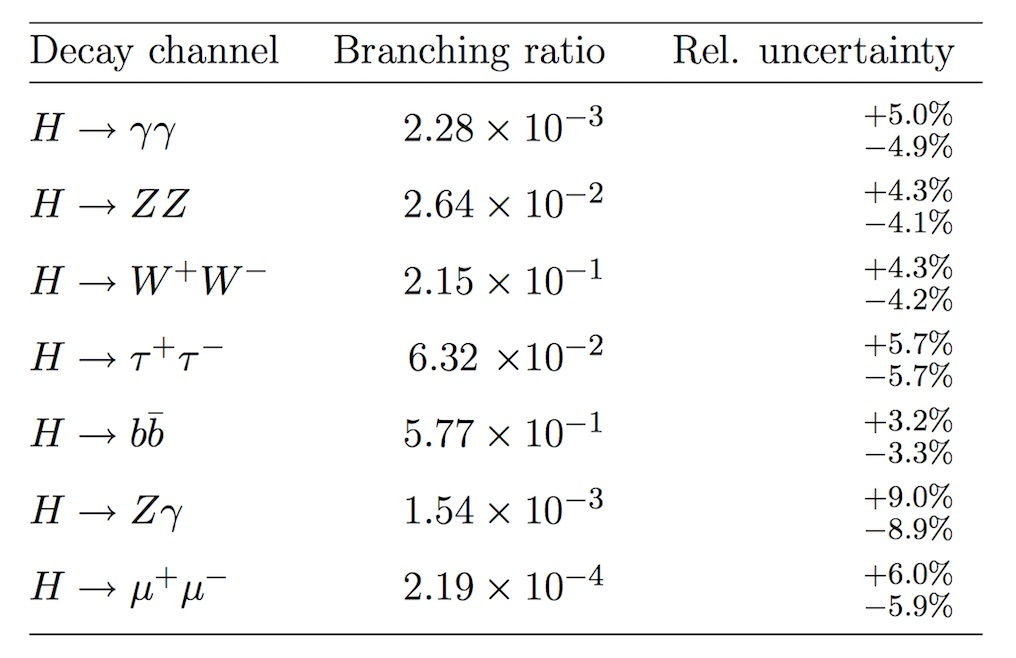
\includegraphics[scale=0.32]{images/Decay Channel.jpg}
\caption{Decay Channels of Higgs Boson \cite{<Cross>}.}
\label{tab:dec}
\end{table}

\vspace{5mm}
\textbf{DECAYS TO QUARKS AND LEPTONS}\\
The first decay we will discuss is Higgs decay into a pair of fermion and an anti-fermion. The Higgs boson interaction strength is proportional to fermionic mass therefore a decay to heavy fermions is more likely to occur as opposed to light fermions. Accordingly, then most probable decay is $\PHiggs \rightarrow \Pqt\Paqt$, although its occurrence is permitted when the Higgs boson mass is more than 2$m_t$ ($\sim$350GeV). With a branching ratio of $\sim$58\%, Higgs commonly decays to $\Pqb\Paqb$ when the mass is $\sim$125 GeV \cite{<PDG>}.\\
Subsequently, Higgs boson decaying into a fermionic pair of $\Pgtp\Pgtm$, that is probed by the decay products of tau leptons. The rest of the most likely decays to fermion anti-fermion pairs such as $\Pgmp\Pgmm$, $\Pcharm\APcharm$, $\APelectron\Pelectron$, can not be exploited yet due to their QCD background signatures or little branching ratio at present integrated luminosity.

\vspace{5mm}
\textbf{DECAYS TO GLUONS AND EWK GAUGE BOSONS}\\
For Standard Model Higgs at mass of 125 GeV, the possible decays are $\Pgg\Pgg$, $\Pg\Pg$, $\PZ\PZ^\ast$ and $\PW\PW^\ast$. In these with biggest branching ratio, $\PW\PW^\ast$ channel has a $\sim$21\% probability. Then is a gluon pair decay which occurs $\sim$8\% of the time. We can not study this decay at present in the collider because it is not distinguishable from the QCD dijet background. The decay into a photon pair is a significant channel for study and search of Higgs boson, but it lacks clear signal over background ratio. Comparatively, diphoton invariant mass has appreciable experimental resolution, where the small Higgs signal is seen as a peak over other backgrounds from either jet signals which are misinterpreted as photons or QCD production of diphotons.\\
The bosonic $\PZ\PZ^\ast$ pair decay has a low branching ratio $\sim$2.6\%, but it is completely reconstructed in the final state and its experimental invariant mass resolution is also favorable. For the final state ($H\rightarrow ZZ^{\ast}\rightarrow 4l$) a good signal over background ratio is detected as the branching ratio decreases even more for decays of $\PZ \rightarrow 4l$. This channel is popularly known as the ``golden channel'', it will be explained in detail in the next section.\ref{subsection:gc} and is mainstreamed in the following thesis.

\begin{figure}[h]
\centering
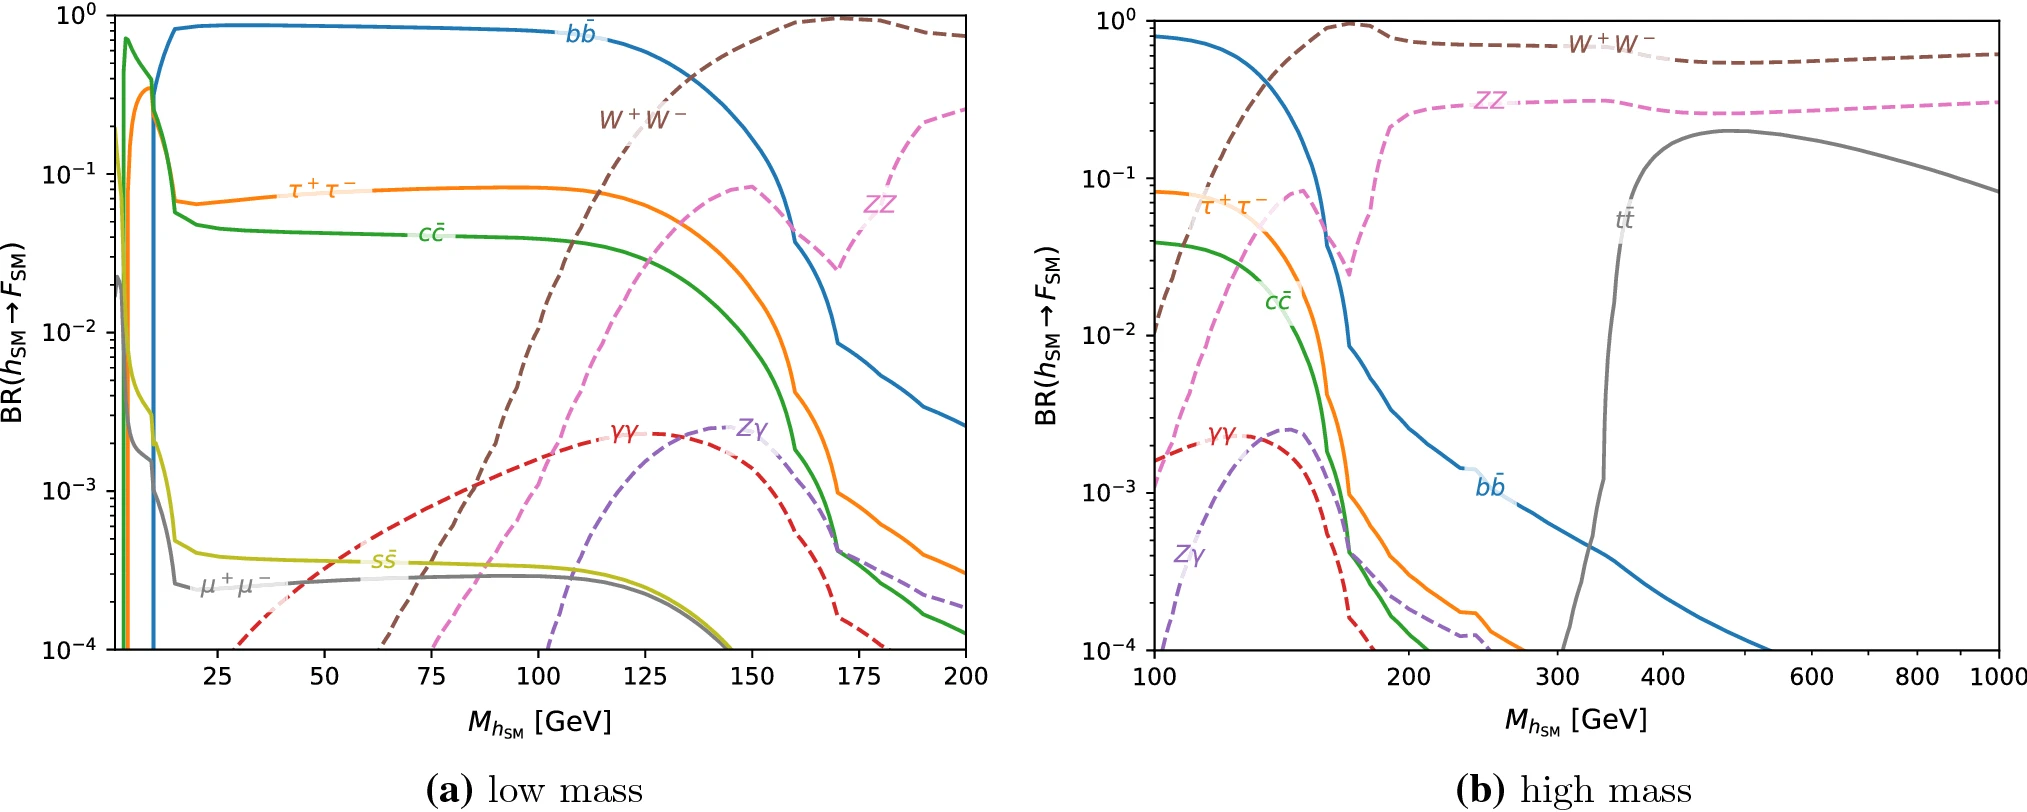
\includegraphics[scale=0.2]{images/BR.png}
\caption{Branching ratios of Higgs decay split into the low mass domain (left panel) and the high mass domain (right panel) \cite{<decaybr>}.}
\label{fig:decaybr}
\end{figure}

\subsection{Golden Channel}
\label{subsection:gc}
In golden channel, Higgs boson decays to a pair of Z vector bosons which in turn decay into electrons or muons pairs, represented as $H\rightarrow ZZ^{\ast}\rightarrow 4l$, directly as $H\rightarrow4l$. Detecting four leptons in the final state that come from Higgs boson decay in our data does not indicate a Higgs boson signal is discovered. There are Standard Model interactions that have similar signature but without the indulgence of Higgs. Most common are two Z bosons or Z\Pgammastar detected by gluon pair fusion or annihilation of quark and anti-quark pair. Another significant contribution comes from reducible background ``Z+X'', where X stands for Z boson reproduced by a pair of leptons, which are not products of Higgs.\\
4\Pe, 4\Pmu and $2\Pe2\Pmu$ are the three considered final states of the decay, with contrasting mass resolution and reducible background rate, therefore analysed separately. The four leptons in final state have a definite signature, hence varying production mechanisms are easily attainable by event jet's extra objects, absent transverse energy and additional leptons. Few of the main production mechanisms have low statistics because of low branching ratio around 0.0124\%, but in HL-LHC Run III this channel is the main tool for measuring properties and Beyond Standard Model (BSM) anomalies.\\
$H\rightarrow ZZ^{\ast}\rightarrow 4l$ is proclaimed ``golden channel'' for the final missing piece: hunt for Higgs boson of SM. The prominent reasons for which are:
\begin{enumerate}
    \item Final state objects are completely reproduced. Even at low energy LHC experiments can reproduce leptons and they can overturn four leptons from final state back to Higgs boson. To discriminate signal from background, kinematic properties of $4l$ like their four momentum are used.
    \item Exemplary momentum resolution. Higgs boson is measurable precisely with the distinct momentum resolution of electrons and muons,
    \item Notable signal to background ratio. There is a $2:1$ signal to background ratio around limited mass region of Higgs boson and low branching ratio.
\end{enumerate}
The golden channel seen in Fig.\ref{fig:golden} has given notable results from CMS and ATLAS collaborations at $\sqrt{s}=13$ TeV e.g.:
\begin{itemize}
    \item Higgs boson mass measurement, apart from the one given in the SM. \cite{<measure>}\cite{<measured>}\cite{<couple>},
    \item Width measurement \cite{<measure>}\cite{<measured>}, jointly analysed in the off-shell and on-shell areas \cite{<width>}\cite{<constraint>}, and for one taken from distance of flight in the accelerator \cite{<limit>},
    \item Signal strength, the observed rate ratio of the Higgs boson to the rate expected in SM and Higgs-fermion and Higgs-gauge boson couplings \cite{<measure>}\cite{<couple>},
    \item Spin-parity, biasing over zero spin and even parity for Standard Model consistency \cite{<measure>}\cite{<study>}\cite{<evidence>}\cite{<cons>}\cite{<diboson>},
    \item Fiducial cross section, unified and also several parameterized functions \cite{<fid>}\cite{<pro>} used in the Standard Model Lagrangian construction of the Higgs boson processes, studying tensorial couplings, uncommon production modes, in analysis of effective form factors, etc.,
    \item Anomalous couplings, interactions test via scattering amplitude of a spin-zero $H$ boson with two spin-one gauge bosons $VV$, such as $gg, \gamma\gamma, ZZ, WW$ and $Z\gamma$ \cite{<limit>}\cite{<cons>}\cite{<diboson>},
    \item Determining other heavy Higgs bosons in $H \rightarrow \Plepton \Plepton \Plepton \Plepton, H \rightarrow \Plepton \Plepton \Pnu \Pnu, H \rightarrow \Plepton \Plepton \Pq \Pq$ and $H \rightarrow \Pnu \Pnu \Pq \Pq$ with Higgs mass spectrum with upper limit extended to 1 TeV \cite{<sear>}\cite{<pair>}.
\end{itemize}
\begin{figure}[h]
\centering
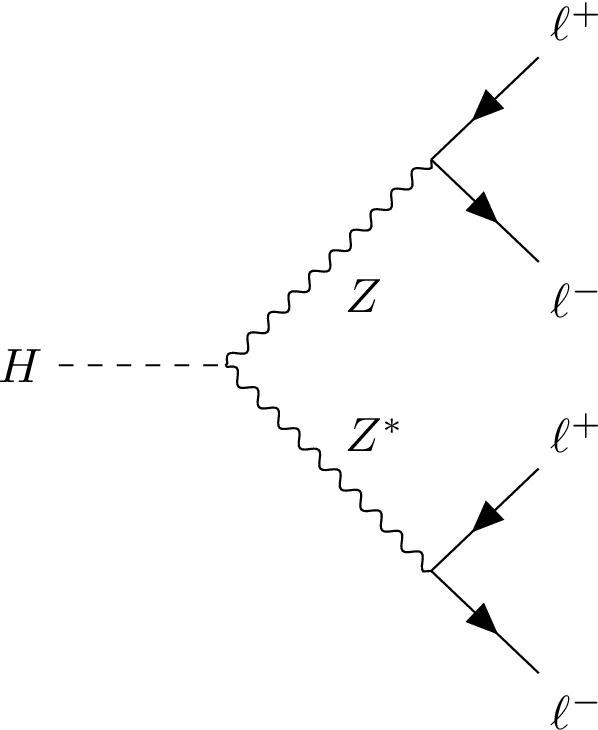
\includegraphics[scale=0.2]{images/goldenchannel.jpg}
\caption{The Golden Channel}
\label{fig:golden}
\end{figure}
\section{Experimental Searches for Higgs Boson}
This section will give brief chronicle search history which led to Higgs boson discovery declared on $4^{th}$ July in 2012 and is at present being authenticated by all purpose machine LHC. LHC's recent measurement results and current searches.
\subsection{Indirect Constraints on the Standard Model Higgs Boson}
Fits to precision measurement of electroweak observables set indirect experimental restrictions on mass of Standard Model Higgs boson. Loop effects in Higgs boson are a major factor in the \PWpm and \PZ vacuum polarization, which generates a logarithmic sensitivity on the ratio of the \PZ and \PWpm bosons masses to the Higgs boson mass. A likelihood fit to the precision electroweak samples collected during past three decades at Large Electron-Positron (LEP) Collider at CERN, Standford Linear Collider (SLC), the Tevatron at Fermilab and other results, gives $m_{H}$=$94^{+29}_{-24}$GeV or $m_{H}<152$GeV at 95\% confidence level (C.L) \cite{<pem>}. Loop effects also make top quark to contribute to the \PWpm boson vacuum polarization which has quadratic effect on the top mass. For top quark, $m_{\Pqt}$=173.2 $\pm$0.9 GeV \cite{<tew>} and for \PWpm mass of 80.385 $\pm$0.015 GeV \cite{<pem>} were considered.
\subsection{Searches for the Standard Model Higgs Boson at LEP}
Higgs-strahlung in the s-channel is the leading mechanism for acquiring Higgs boson in $\Pep\Pem$ collisions at LEP energies, $\Pep\Pem \rightarrow \PHiggs\PZ$. Final state \PZ boson is either virtual (LEP1 ), or on mass shell (LEP2). Higgs boson production via $\PWplus\PWminus$ and $\PZ\PZ$ interaction in the t-channel at LEP energies, has a small cross section. Higgs boson in LEP searches is sensitive to variation in center-of-mass energy, $\sqrt{s}$. During the LEP1 phase, mass of the SM Higgs boson was approximately 65 GeV bounded from below  \cite{<jane>}. At LEP2, data samples were generated in huge amount at $\sqrt{s}=209$GeV. At LEP1, production modes such as $\PZ \rightarrow \Plp\Plm$ and $\PZ \rightarrow \Pgn\Pagn$ were used as other channels were restricted by the backgrounds. Where as LEP2 used all decay modes in data accumulation.
\subsection{Searches for the Standard Model Higgs Boson at Tevatron}
In the Tevatron, principal production interactions were: gluon fusion $\Pg\Pg \rightarrow \PHiggs$, associated vector boson production ($\PWpm\PHiggs$ or $\PZ\PHiggs$) and vector boson fusion (VBF). Some channels were optimised for VBF because it has a smaller cross section. Compared to LEP analyses, Tevatron has lower signal-to-background ratio, although the systematic uncertainties on the calculated background signals are generally larger than the signal rates \cite{<RPP>}.
\subsection{Searches for the Standard Model Higgs Boson at LHC}
At hadron colliders, production mechanism depends on the principle of mass-Higgs coupling, i.e couples more strongly to heavy particles which are the top quark, vector bosons (\PZ, \PW) and the bottom quark. The Feynman diagrams of the four main production modes which are displayed in Fig.\ref{fig:pm} and Fig.\ref{fig:Cross}, in which dominant production process is gluon–gluon fusion mechanism. This is followed by the $\PW\PW$ and $\PZ\PZ$ fusion process, for large $m_{H}$ values it can reach $gg$ fusion cross section. The cross sections for the $\Pqt\Paqt$ pairs and associated production with \PW/\PZ bosons are one to three orders of magnitude less than the $\Pg\Pg$ pair and for mass range $m_{H}\le250$ GeV these interactions are relevant.

\chapter{Compact Muon Solenoid}
This chapter will dissect the LHC machine which accelerates particles at a speed close to the speed of light before they collide with each other. The aim of Run II of LHC was to study all Higgs production modes, decay modes and accuracy in studying its properties. Also if there are deviations in the data accumulated from the one predicted in Standard Model which will mark new physics such as supersymmetry, dark matter and dark energy, antimatter deficit compared to matter and how quark-gluon plasma are the source behind particles that make the matter of Universe. We have used Monte Carlo (MC) samples produced from Run II from 2016 till 2018 in our thesis for data analysis.\\
\section{Large Hadron Collider}
Large Hadron Collider (LHC) is the world's biggest and most dynamic machine ever built. It is absurd, as the world's largest machine was built to comprehend the smallest particle known to mankind. It runs approximately $\sim$100m underground and travels 27 km in circumference which consists of superconducting magnets and accelerating compartments, shown in Fig.\ref{fig:lhc}, which give the particles an energy boost along the path. It accelerates two beams of protons, circulating the ring, in opposite directions induced with ultrahigh vacuum. These protons are circulated by the strong magnetic field used for ‘bending’ and a series of other magnets that are used for controlling and focusing the beams. The superconducting magnets are made from electric cables which reduce energy loss and resistance in superconducting state. When the particles are just about to collide a magnet is used to ``squeeze'' the particles in the beam's cross section to increase the collision rate known as integrated luminosity.\\
\begin{figure}
    \centering
    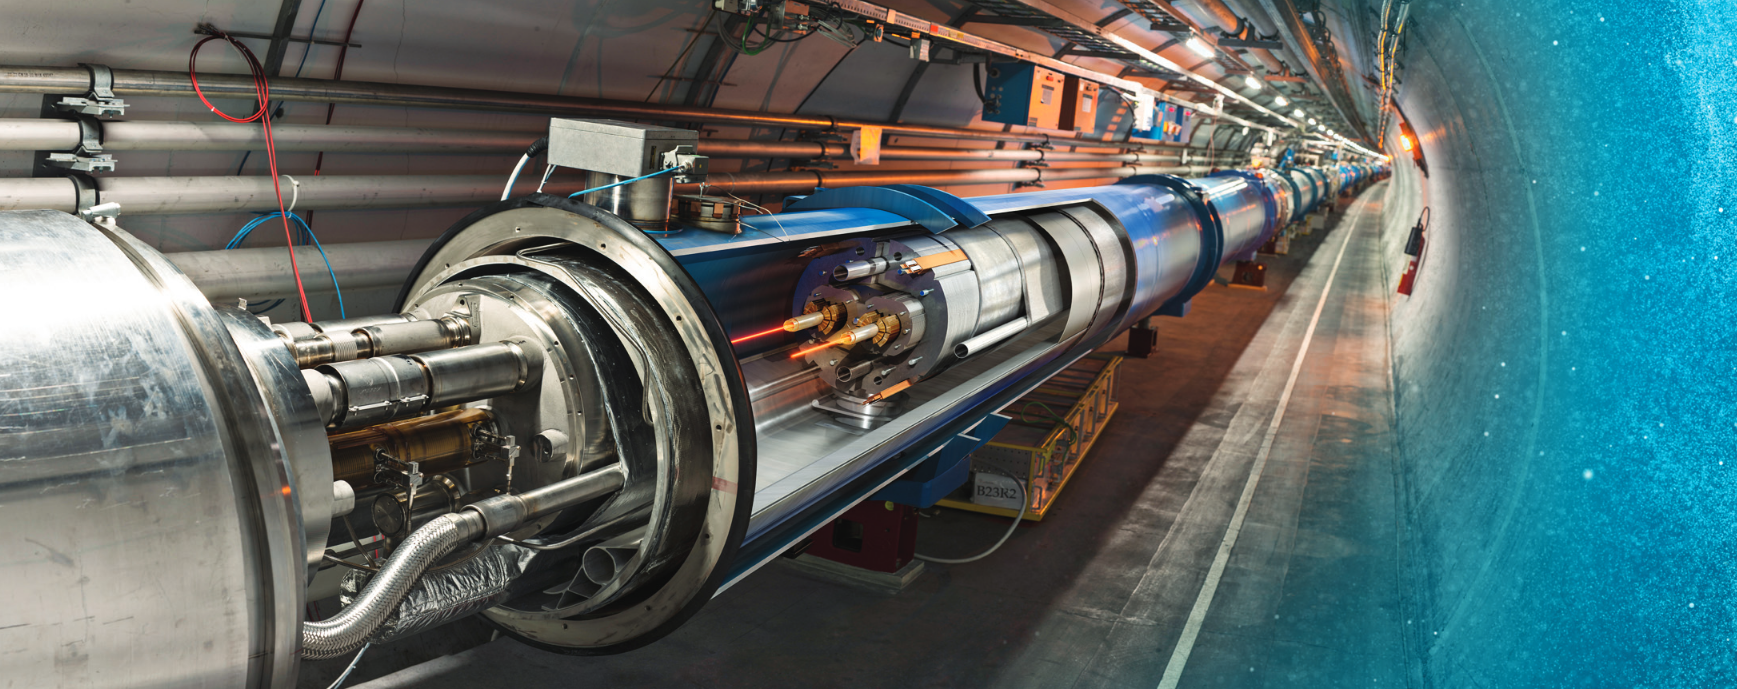
\includegraphics[scale=0.26]{images/lhci.png}
    \caption{LHC at CERN, Geneva}
    \label{fig:lhc}
\end{figure}
Protons are accelerated up to the necessary energies, through a series of smaller accelerators shown in Fig.\ref{fig:accom}. The process starts with the 50 MeV LINAC2 which shoots the protons into a multi-ring booster synchrotron that accelerates them up to 1.4 GeV. After which the protons are directed to the Proton Synchrotron (PS) machine accelerating the particles up to 26 GeV and generate the bunching and spacing that the LHC requires. To accelerate the beam from 26 GeV up to 450 GeV the beam is then injected into the Super Proton Synchrotron (SPS). In the SPS the protons are fed into one of the LHC rings. Before the LHC accelerates these protons up to their final energies, this process is repeated 24 times, 12 times to fill each of the two rings. Once the LHC has accelerated these proton bunches to their final energies, the beams are gradually brought together so that they will collide inside the four experiments. \\
\begin{figure}[h]
\centering
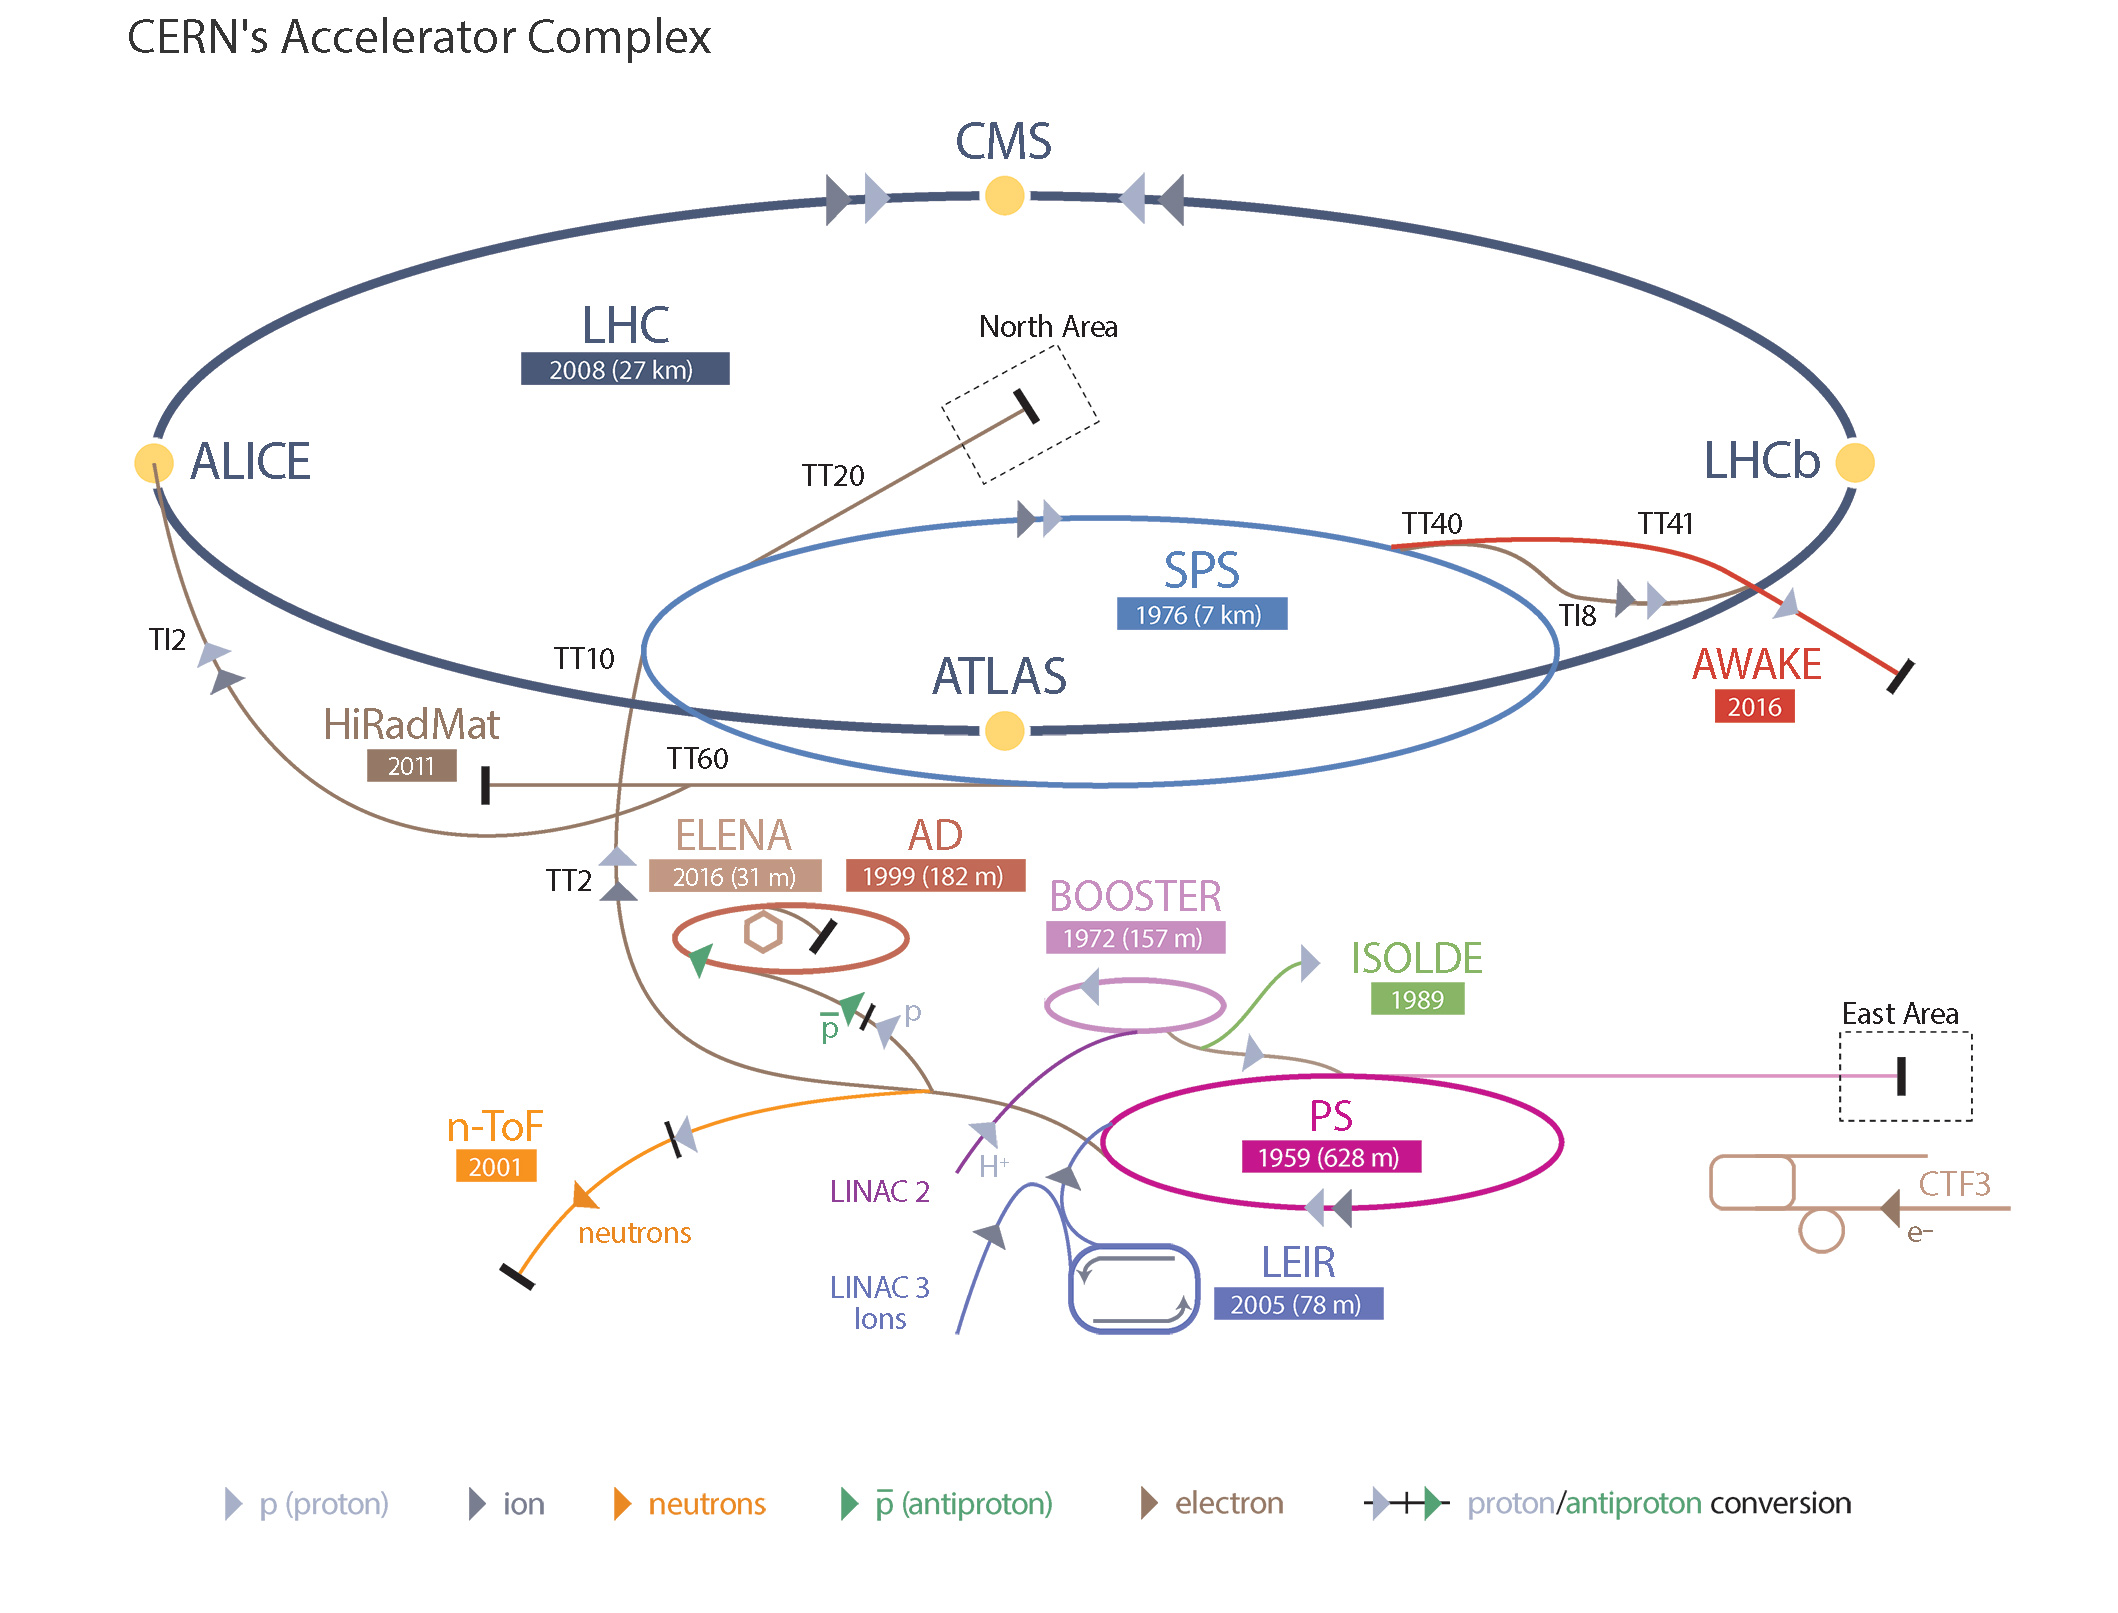
\includegraphics[scale=0.1]{images/acc.jpg}
\caption{This CERN accelerator complex. Experiments at LHC: ALICE, ATLAS, CMS, LHCb \cite{<acc>}.}
\label{fig:accom}
\end{figure}
Theses detectors observe and categorize the particles that are produced when these protons (ions) are collided with each other. Currently, the four experiments at the LHC are: The Compact Muon Solenoid (CMS), A Toroidal LHC Apparatus (ATLAS), Large Hadron Collider beauty (LHCb) and Large Ion Collider Experiment (ALICE). The ATLAS and CMS detectors are high luminosity, all-purpose detectors constructed to test many different aspects of the SM, including the Higgs boson. LHCb looks specifically at bottom (beauty) quark interactions and while ALICE is designed for ion collisions.
\section{CMS Detector}
Compact Muon Solenoid as shown in Fig.\ref{fig:dec} is a multipurpose detector where its key characteristics are defined in its name:
\begin{itemize}
    \item \textbf{Compact}: it has small dimensions compared to its mass, a compact detector as the tracker and calorimeter are within superconducting coil.
    \item \textbf{Muon}: it has advanced muon detection system, it is developed with muons triggers and muon chambers which detect muon signatures for events such as; Higgs decays to four muons.
    \item \textbf{Solenoid}: solenoidal superconducting magnet, the largest solenoid magnet (B = 4T) in the world which is producing a field 100,000 times the Earth's magnetic field.
\end{itemize}
\begin{figure}[h]
\centering
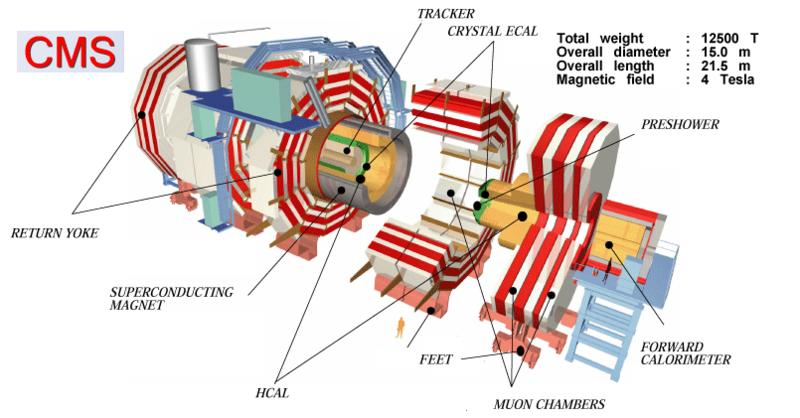
\includegraphics[scale=0.4]{images/9803027.jpg}
\caption{The CMS Detector \cite{<cms>}}
\label{fig:dec}
\end{figure}
\subsection{Tracker}
Tracker is the central hollow vacuum path of the LHC, with silicon sensors that are finely segmented. These silicon pixels and silicon strips, track charged particles and measure their momenta. They can also give the positions of decay of long-lived unstable particles. The CMS silicon tracker consists of two tracking devices which utilize semiconductor technology: the inner pixel and the outer strip detectors.\\
The tracker detector is in the middle of CMS, where the beams collide in the range of 4cm to 110cm in radius and $\sim$280cm along the beam axis. The CMS tracker is built to reproduce objects such as high $p_{T}$ hadrons, muons and electrons along high precision and an apt resolution of momentum. Decay vertices of long-lived unstable particles can also be measured. This is the reason behind the use of all-silicon for the tracking system. Charge particles are tracked and their momentum is efficiently measured by the finely segmented silicon sensors. The CMS tracking system is illustrated in Fig.\ref{fig:CMS Tracking System}.
\begin{figure}[h]
     \centering
     \begin{subfigure}[b]{0.45\textwidth}
         \centering
         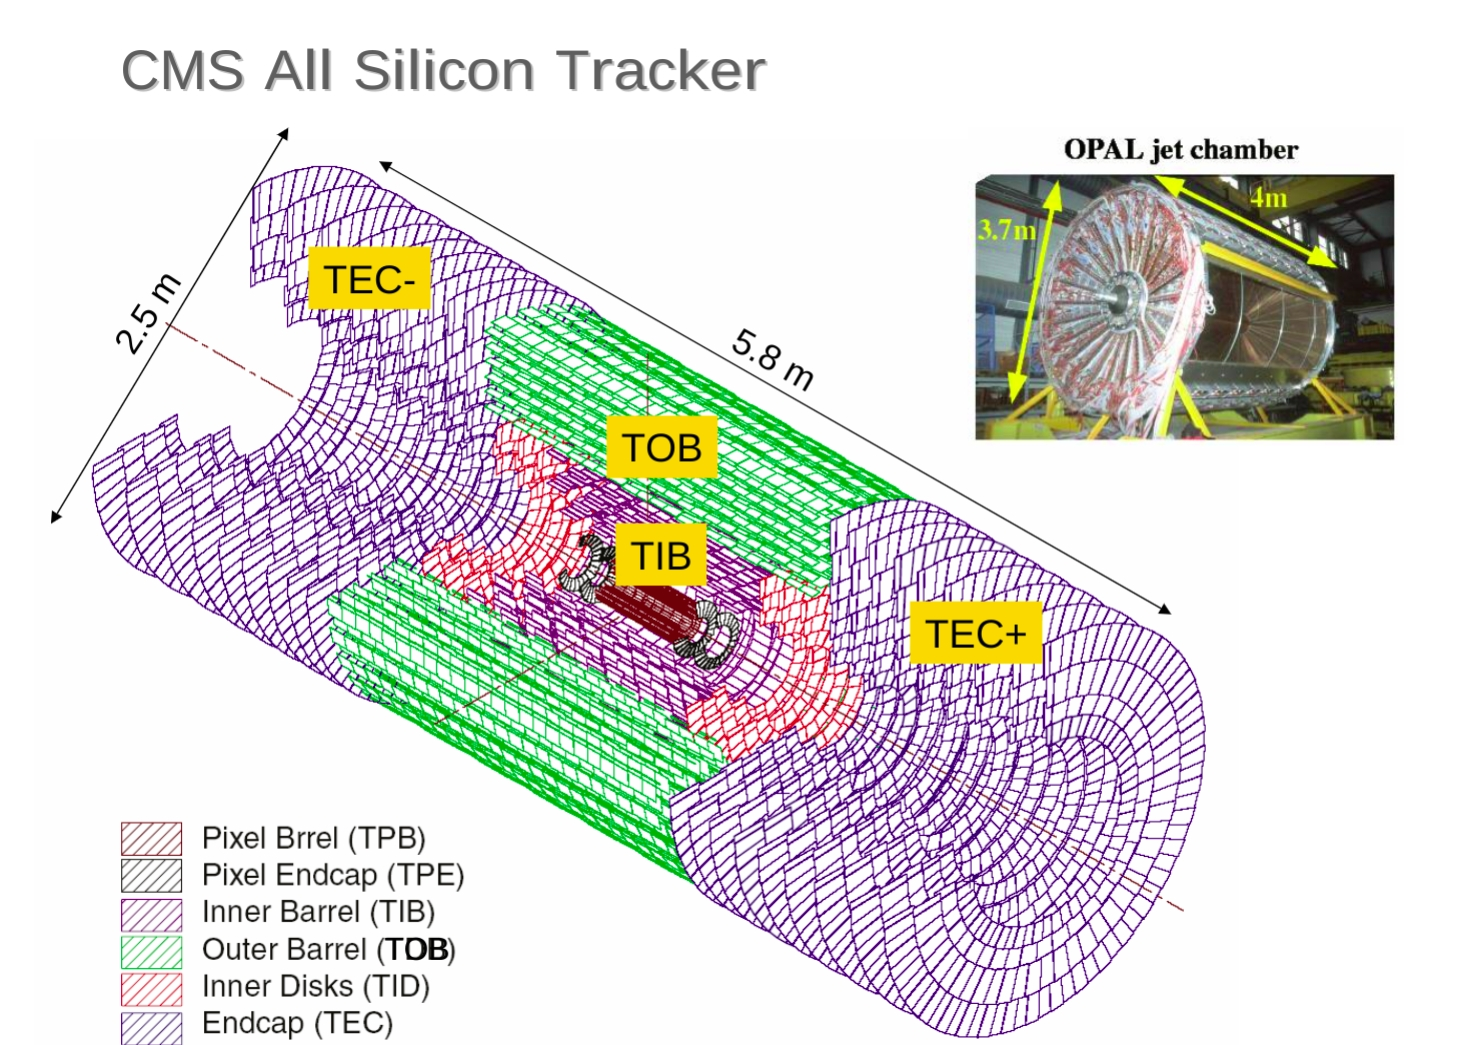
\includegraphics[width=\textwidth]{images/Track1.jpg}
         \caption{The Tracking System}
         \label{fig:track1}
     \end{subfigure}
     \hfill
    \begin{subfigure}[b]{0.45\textwidth}
         \centering
         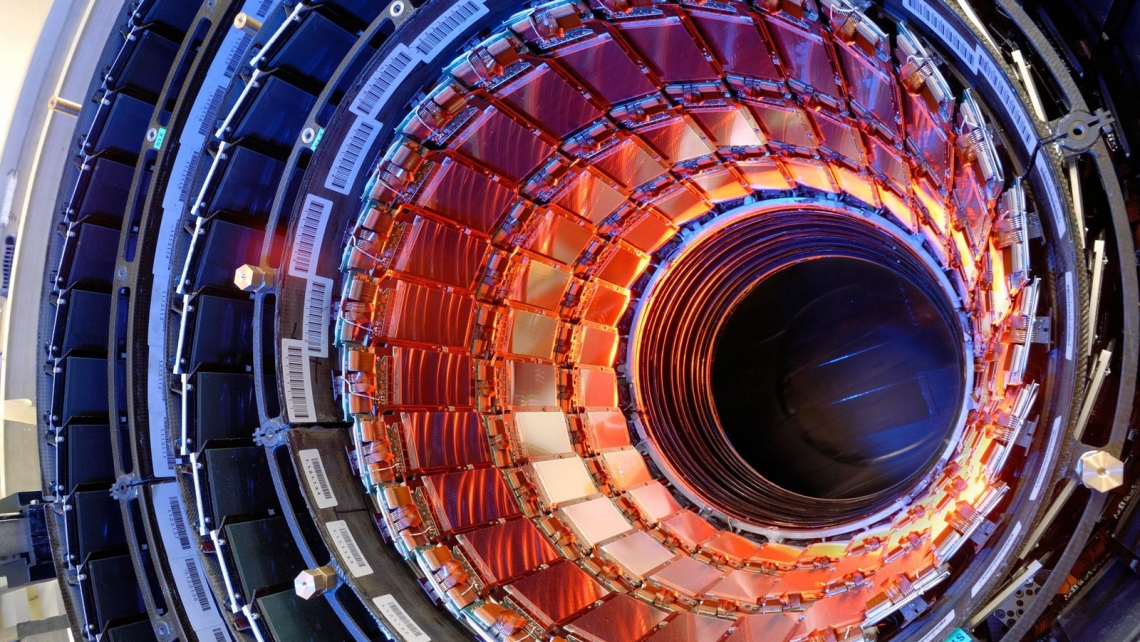
\includegraphics[width=\textwidth]{images/Track2.jpg}
         \caption{CMS Tracker}
         \label{fig:track2}
     \end{subfigure}
     \hfill
     \caption{Visualising CMS Tracker}
        \label{fig:CMS Tracking System}
\end{figure}
The tracker covers the region with pseudorapdity (the particle's angle relative to the beam axis) $|\eta|< 2.5$. High $p_{T}$ resolution tracks are reproduced  $\delta P_{T}$ /$P_{T}$ = (15$P_{T}$/TeVc + 0.5) in the core area $|\eta| < 1.6$, with resolution $\delta P_{T}$ /$P_{T}$ = (60$P_{T}$ /TeVc + 0.5) when $|\eta|\sim$ 2.5.
The inner pixel device contains $4.4 \times 10^{6}$ pixels as a square with each side 150 µm in length. The resolution of dimensions is 15 µm. The outer strip device includes strips amounting to $25 \times 10^{3}$. The barrel has ten strip layers and three pixel layers. Where as the endcaps have nine outer forward silicon detectors (TOB), three inner discs (TID) and two pixel layers.
\subsection{Electromagnetic Calorimeter}
The (ECAL) electromagnetic calorimeter has been equipped to accurately detect positions and energies for photons and electrons. It also measures the energies from the showers of hadrons and jets which deposit portion of their energies in ECAL. The ECAL is a homogeneous calorimeter and its crystals are made up of lead tungstate (PbWO4). It has small radiation distance ($X_0 = 0.89 \times 10^{-2}$) and an enormous density ($8.2 g/cm^3$), and small Moli`ere radius ($R_{M} = 2.19 \times 10^{-2}$). Endcap (EE) and barrel (EB)  are the two regions of the ECAL. The EB encompasses the domain $|\eta| < 1.48$ and has 61,000 crystals. There are 36 superunits in the EB, and every unit consists of four modules illustrated in Fig.\ref{fig:e1}. Every crystal of lead tungstate consists of front facing area of 22 × 22 $mm^2$ and 26 × 26 $mm^2$ back area and all of them are 23 cm long, about 26$X_0$. Lead tungstate crystals are tilted along the beam axis at $3^{\circ}$. Avalanche photo diodes (APD) comprehend signals computed behind the crystals in the EB. The EE covers area between $1.5 < |\eta| < 3.0$. \\
\begin{figure}[h]
     \centering
     \begin{subfigure}[b]{0.55\textwidth}
         \centering
         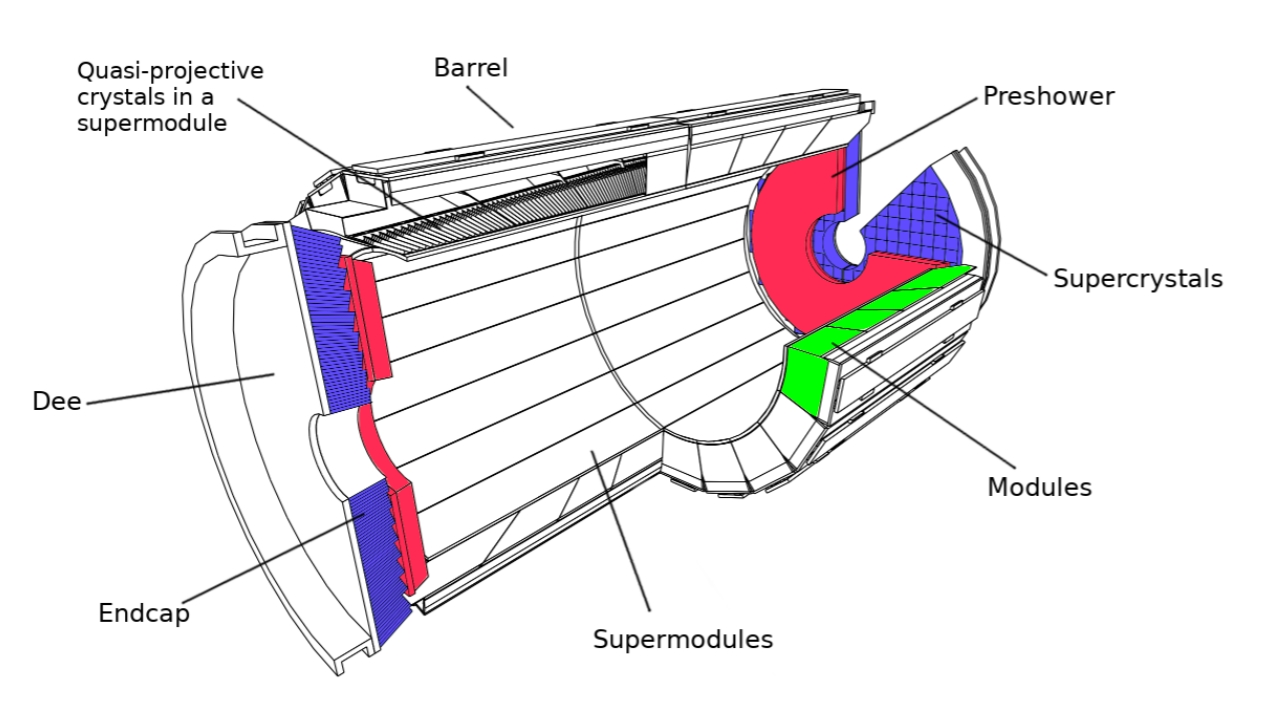
\includegraphics[width=\textwidth]{images/ecal1.jpg}
         \caption{ECAL Geometry}
         \label{fig:e1}
     \end{subfigure}
     \hfill
    \begin{subfigure}[b]{0.4\textwidth}
         \centering
         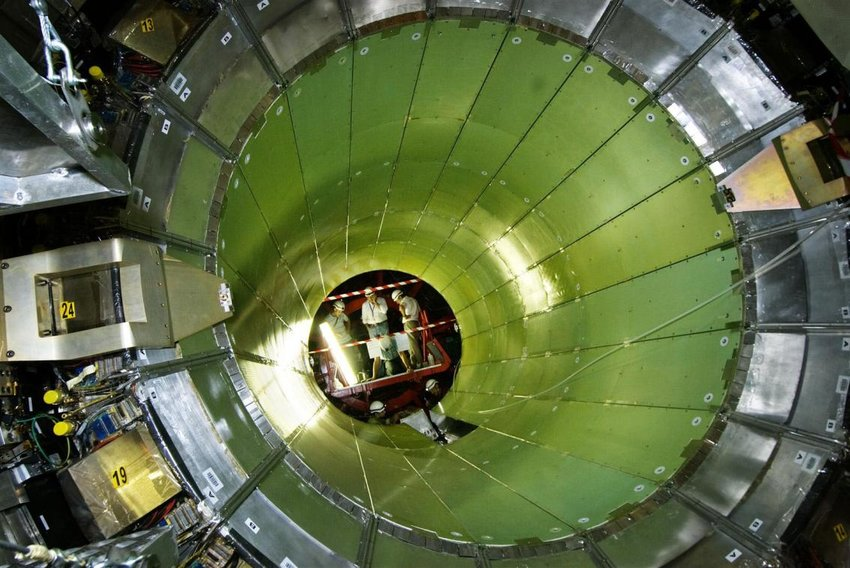
\includegraphics[width=\textwidth]{images/ecal2.png}
         \caption{Insertion of the last CMS ECAL supermodules in the ECAL Barrel}
         \label{fig:e2}
     \end{subfigure}
     \hfill
     \caption{Electronic Calorimeter}
        \label{fig:ECAL}
\end{figure}
EE has 73000 crystals and vacuum photo triodes (VPT) are used for reading the signals at crystal's back in the EE. At the face of EE, a preshower detector (ES) covers the area between $1.6 < |\eta| < 2.6$. The construction helps in dismissing $\Ppizero$ which decays into two photons. The ES minimizes this particular background in the channel where Higgs boson decays to a photon pair \cite{<ecal>}.
\subsection{Hadronic Calorimeter}
The hadronic calorimeter (HCAL), along ECAL, is also used to identify jets, hardrons and give their energy measurements. It is made up of 36 wedges, each of which weighs as much as 6 African elephants. The HCAL consists of four sub-sections: hardron barrel (HB), hadron endcap (HE), hadron outer (HO) and hadron forward (HF). In between the superconducting solenoid and ECAL the HB and HE are placed. Brass and plastic scintillating plates are the interchanging layers of which both HB and HE are made from. The HB takes over area defined by $|\eta| < 1.4$, while the HE covers area between $1.5 < |\eta| < 3.0$. Every HB tower projects a region of $\triangle\eta \times \triangle\phi$ = 0.087 × 0.087. Scintillating plates are inserted with wavelength-shifting (WLS) fibers. Light accumulated from these are detected by Hybrid Photo Diodes (HPD). Also, HB interaction length is 5.8($\lambda_I$ ) at $\eta$ = 0.\\
\begin{figure}[h]
\centering
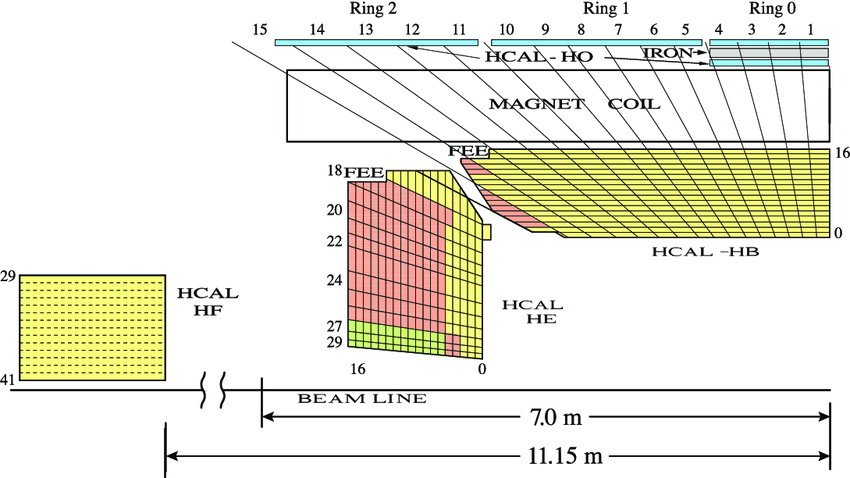
\includegraphics[scale=0.4]{images/hcal.png}
\caption{Hadron Calorimeter}
\label{fig:hcal}
\end{figure}
The tails of hadronic showers can be detected by the HO which HB cannot collect. Located in the middle of the magnet and muon system, the HO is a flash detector. It encompasses the area $|\eta| <1.26$.
At the end of HCAL, HF is located at $3.0 < |\eta| < 5.0$, which is outside the solenoid. It is built from quartz fibers which is the active medium and steel which is the absorber. Quartz fibers can tolerate the harshness of radiation, as forward calorimeters have to face particle flux of unmatched strength by the use of short fibres (1.43m) and long fibres (1.65m). The short fibers are at the front of CMS and are 22cm deep. They are placed here to detect showers created by photons and electrons. Hadrons produce signals in both segments of HCAL, leaving large traces of their energy in the 22cm depth of short fibers. HF calorimeters are built to check jets coming with high energy to an accuracy of 20\% to 30\% at 1 TeV \cite{<hcal>}.
\subsection{Superconducting Solenoid}
The experiment is built around CMS magnet. The superconducting magnets bend the trajectories of charged particles along the radius of CMS arising from the interaction point. The complication of this can be visualised by imagining the firing of two needles having 10km distance between them and even then, the interaction is as accurate as them meeting halfway but not combusting in one another. The momentum resolution of the particles can also be estimated, since the particles with high energies have less bent paths by the magnetic field. The energy loss due to magnet is reduced by cooling them to a temperature of -271.3$^{\circ}$C by liquid helium.\\
The superconducting solenoid is made of 1232 dipole magnets 23m long for bending of the beam, quadruple magnets which are 392 in amount and 5-7m in length are used for focusing the beam. The liquid helium around the solenoid, allows 19.14 kA current to flow through with negligible resistance. The flux comes back along an iron yoke containing five wheels and two end caps, each carrying three disks. The yoke mainly makes the field more homogeneous in the tracker and reduces the straying of the field by giving back the solenoid its magnetic flux. For precise reproduction and Monte Carlo (MC) event simulation, cosmic muons are used for a detail map of CMS magnetic field. The accuracy of the tracker magnetic field that has been mapped is more than 0.1$\%$.
\subsection{Muon System}
Muons are mostly seen as the end products of numerous interactions occurring at the LHC experiment. Muons travel along the whole CMS, scarcely any ionization is left along the path making it easier for muons to be identified. Recognizing muons properly and reproducing their momenta precisely, were the main construction factors in the experimental setup. The muon detecting system entails three section branching, with iron return yoke plates that allow only neutrinos and muons to transverse through: Cathode Strip Chambers (CSC) inside endcap area, Drift Tubes (DT) inside barrel area, and Resistive Plate Chambers (RPC) inside the endcap and barrel area as shown in Fig.\ref{fig:tms}.
\begin{figure}[h]
\centering
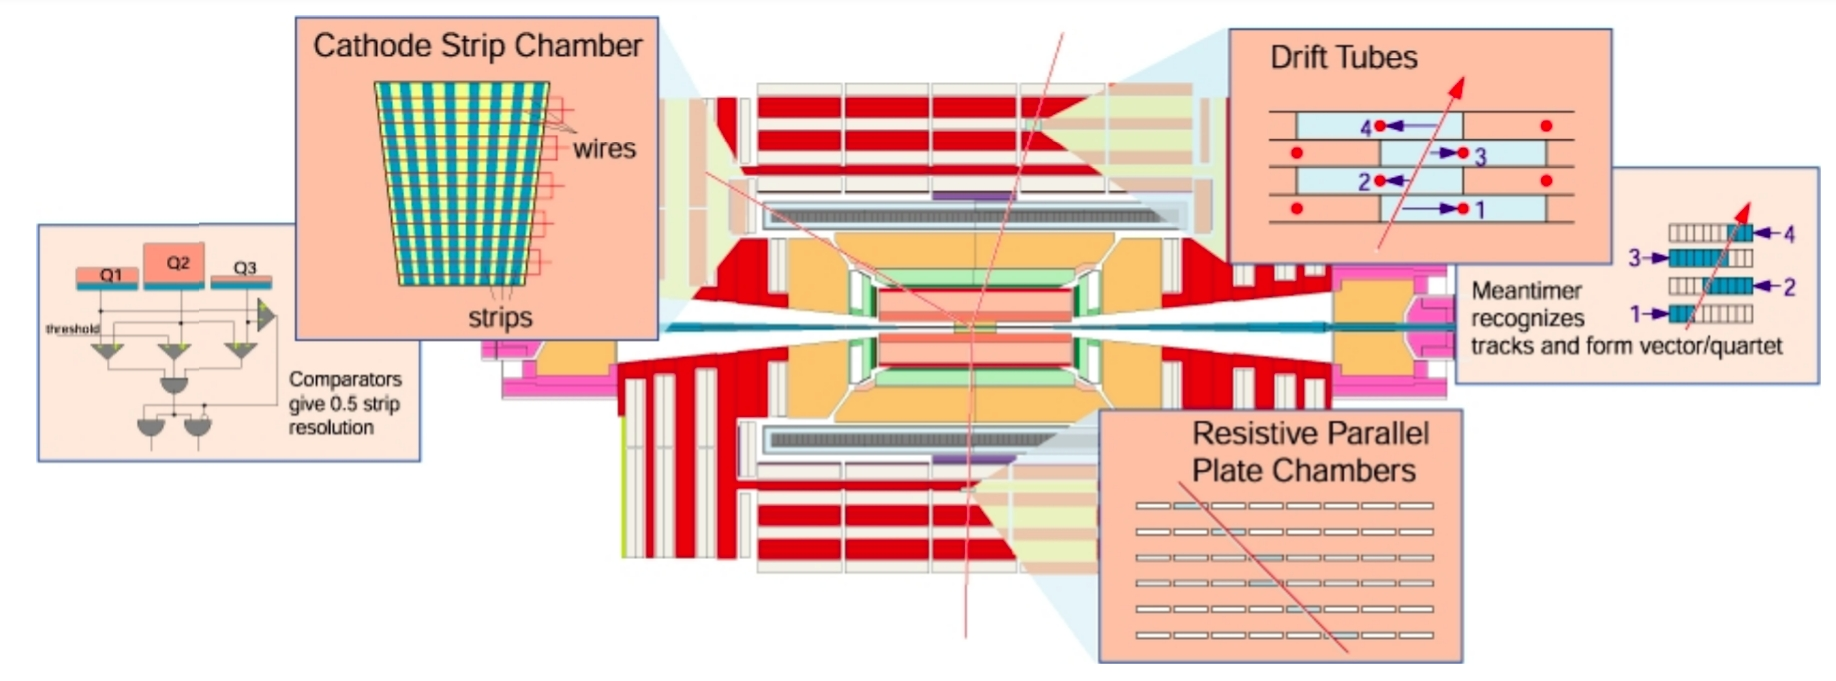
\includegraphics[scale=0.2]{images/ms}
\caption{The Muon System}
\label{fig:tms}
\end{figure}
The CSC and DT give accuracy in position checks while time measurements are identified using RPC.\\
\subsection{Pattern Recognition}
All particles except electron proton and neutron produced in CMS are generally unstable and they decay into lighter, more stable and well identified particles. Particles transversing along the tracker leave their characteristic signatures (patterns), after which they are uniquely identified in each layer they pass through. If any new particle is present or not can then be concluded, as shown in Fig.\ref{fig:patt}.\\
\subsection{Trigger System}
A trigger is a system which decides the events selection when specific number of events of the total can be recorded. Each detector has its own trigger system; Level-1 (L1) system is based on electronics and High Level Trigger (HLT) system is based on reconstruction software. For better probability of rare particle production, e.g. Higgs boson, bunch of protons are made to have $4 \times 10^{7}$ collisions per second. The different particles signatures resulting from these interactions are computed with high precision to save (or ‘trigger on’) events ($\sim 100/s$) which confirm Standard Model elementary particles and verify new physics, i.e. $\PHiggs \rightarrow ZZ^{*} \rightarrow 4l$. The event rate is therefore decreased to a tractable level. Subsequently, detailed analysis is performed on these separated events.\\
\begin{figure}[h]
\centering
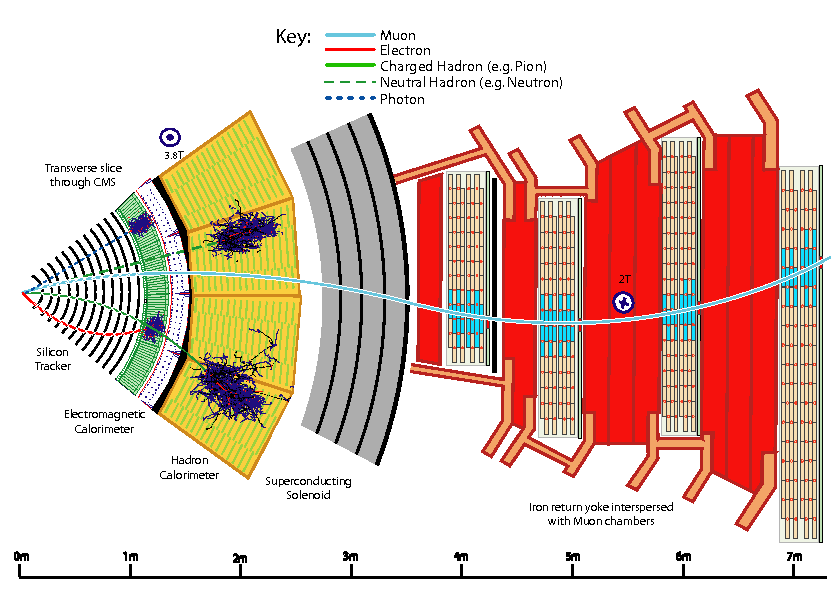
\includegraphics[scale=0.4]{images/pattern.png}
\caption{Pattern Recognition}
\label{fig:patt}
\end{figure}
\section{Co-ordinate System}
For object reconstruction in CMS experiment there is a standardized coordinate system. The centre point of the accelerator is the origin, x axis is directed towards the centre of the LHC ring, y axis points above and the z axis coincides with the beam direction, overall a 90$^{\circ}$ coordinate system. It is a cylindrical coordinate system; the x-y plane representing the transverse plane, azimuthal angle $\phi$ is measured between x axis and the x-y plane in the domain [$-\pi,\pi$] and lastly, the polar angle $\theta$ is calculated from the z axis in the domain [0, $\pi$].\\
The transverse plane displays the trajectories of particles in search for physics Beyond Standard Model (BSM). The y and x components of momentum and energy are measured at $90^{\circ}$ to the principal axis for for momentum and energy values (for massless particle $E_{T} = p_{T}$). The magnitude of projection vector of any transverse momentum $p_T$ component p onto transverse plane is given as:
\begin{equation}
    \label{eq1}
    P_{T} = \sqrt{P_{x}^{2}+P_{y}^{2}}
\end{equation}
The particle rapidity is calculated as:
\begin{equation}
    y = \frac{1}{2}ln\frac{(E+p_{z})}{(E-p_{z})}
\end{equation}
and when mass is neglected when compared to energy, m/E$\ll$1, it approaches the pseudo-rapidity:
\begin{equation}
    \eta = \frac{1}{2}ln\frac{(E+p_{z})}{(E-p_{z})} = -\frac{1}{2}tan\frac{\theta}{2}
    \end{equation}
which we will use in our thesis for electrons and muons. As the detector has cylindrical shape, the coordinate $\eta$ makes the contrast between two of the sub-detectors: 2 forward sections on opposite sides known as ``endcaps" and the central part ``barrel".\\
$\triangle R$ demonstrates the azimuthal angles $\phi_{i}$, which gives the angular distance between two particles, and pseudo-rapidity $\eta_{i}$, which is written as:
\begin{equation}
    \triangle R = \sqrt{(\eta_{1}-\eta_{2})^{2}+(\phi_{1}-\phi_{2})^{2}}
    \end{equation}
Total transverse energy calculation shows disparity, when a particle escapes the detection, this disparity is expressed as the transverse missing momentum $p^{miss}_{T}$. It is the total negative momentum of projection of reproduced objects on the x-y plane, and in the hermetic (sealed) detector, it is concluded to be the sum of neutrinos $p_T$. 

\chapter{Signal Strength Modifier}
If there is a predictive theory, as the Higgs field in the Standard Model for any given (but a priori unknown) Higgs boson mass, the rate of events will predict that a statistical analysis should see if the theory is true. This chapter will give a brief review of the analysis techniques used to reconstruct Higgs signal and determine signal strength modifier using the CMS results, and also checks if hypothesis tests are compatible with the statistical techniques.  This will ensure the validity of the data collected for Higgs boson mass and will help in categorizing events which are accumulated in the detector. 
\section{Hypothesis Testing in Research Study}
If the measured event rate in a search is more than the expected event rate, than the Standard Model theory is untrue (i.e. there is no Higgs boson, at least not at that mass). For verification of a theory, the expected event rate and measured event rate should have 99.99994\% coincidence level after background reduction which can be achieved when there is unlimited amount of data.\\
Now we not only see if the new particle (or whatever) is actually there, but also if it is there at a rate in agreement with the prediction of its origin. For that we need to decide that, statistically how close the measured rate is to the predicted one.\\
The “rate” is the one that appears in  Poisson probability as $\lambda$ in $p(k|\lambda)=\lambda^{k} e^{-\lambda}/k!$, this gives the probability of having seen $k$ events, when our theory told us to expect $\lambda$. (This picture is complicated by systematic
uncertainties, which are not perfectly defined, but one with uncertainties of its own). In the direct prediction from the theory, we usually have $\lambda=s+b$, where $s$ is expected rate from the signal process, and $b$ is the expected rate from background processes (assumption: both don’t interfere).
The signal strength modifier is a number, usually denoted by $\mu$ which is multiplied to the standard, predicted signal rate: $\lambda \rightarrow \lambda'=\mu s+b$ . This allows that at 95\% statistical uncertainty and the 125 GeV Higgs boson production rate is between 80\% and 130\% of the Standard Model value, i.e. still statistically
very compatible with the SM.\\
Those bounds would correspond to $\mu=0.8$ and $\mu=1.3$ respectively. Much more exciting would be a limit range that did not include 1; that would imply a deviation from the Standard Model after which codes and systematic constraining methods should be double checked.
Statistics here follow Poisson trends, so if we have a high rate, the statistical uncertainty on assessing that rate will be small and so assuming that various systematic uncertainties have been brought under control we can test the theory in some precision very rapidly, but if the rate is low then its uncertainty will be relatively large and harder to pin down. The more data we take, the better the statistical constraint will be \cite{<quora>}.\\
Note also that likelihood and signal strength are directly connected: values of $\mu$ that take
$\lambda$ closer to the observed rate will get a high likelihood, while those that predict rates far
from the observed can be ruled out. We draw a 2D plot of $\mu$ versus a fixed threshold likelihood of 95\% used above and mark the values of $\mu$ where it’s crossed.
\section{Hypothesis Testing of Higgs Signal}
The search for the $\PHiggs \rightarrow \Pmuon + \APmuon$ signal can be formulated as a hypothesis test. The null or background only hypothesis explains the case where only the known SM backgrounds exist, but no signal is present. The other hypothesis is that the background and the signal we are looking for both exist. The modified frequent method or $CLs$ method \cite{<cls>} is used to quantify which hypotheses are favored or excluded.\\
All hypotheses that are considered in this analysis can be expressed as $\mu s+b$, where $\mu$ is the so called signal strength parameter. The signal with background hypothesis corresponds to $\mu$=1 and $\mu$=0 is for the background hypothesis for a Standard Model Higgs boson decay. To estimate the level of compliance of a hypothesis in question, with the measured data, we propose a test statistic $\PSq_{\mu}$. It is a function containing events (signal and bakgrounds) and the standard parameter, in our case the signal strength $\mu$. It is constructed in such a way that a higher value of $\PSq_{\mu}$ indicates a higher incompatibility amongst the data and the chosen $\mu$-hypothesis.
The p-value, defined as the probability of statistics kept for checking is equal or more than the one observed, for a given hypothesis is then calculated to quantify this disagreement. This is illustrated in Fig.\ref{fig:asym}(a). To calculate a p-value the probability distribution function is integrated over all values of $\PSq_{\mu}\ge\PSq_{\mu,obs}$
\begin{equation}
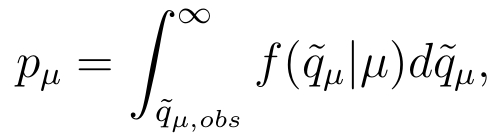
\includegraphics[scale=0.3]{images/1.jpg}
\end{equation}
here $\PSq_{\mu,obs}$ is the number observed from data of the statistics we used for checking and gives the probability distribution function (PDF) of $\PSq_{\mu}$. This PDF has been probed by Monte Carlo pseudo-experiments, where repeatedly Poisson distributions of $m_{\mu\mu}$ according to the hypothesis have to be generated and corresponding test statistic is then computed.\\
For Higgs analysis log-likelihood ratio is used:
\begin{equation}
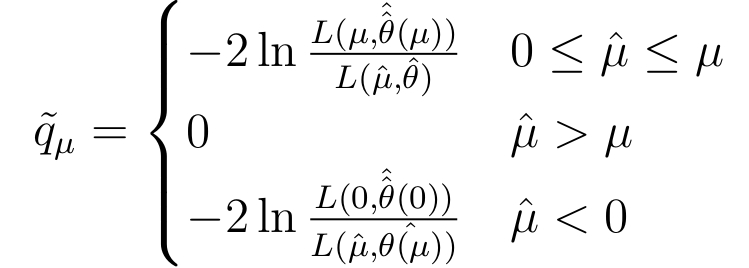
\includegraphics[scale=0.3]{images/2.jpg}
\end{equation}
The likelihood $L$ is based on the best fit of both, signal model and background model put together to the $m_{\mu\mu}$ spectrum. In the formula for the test statistic, $\theta$ are used but are not of interest themselves, the so called nuisance parameter. $\hat{\mu}$ and $\hat{\theta}$ are the best fit values for $\mu$ and $\theta$ floating free in the fit. $\hat{\theta}$ is calculated by a fit with a fixed $\mu$, but floating $\theta$.
In particle physics we commonly change the p-value into an equivalently important $Z$. The local significance of a deviation from the null hypothesis is calculated from $p_{0}$ , the corresponding p-value. It is defined when a standard Gaussian distributed variable, is seen as $Z$ standard deviations more than its mean, with an upper tail probability equivalent to $p$ given as,
\begin{equation}
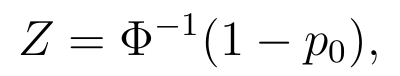
\includegraphics[scale=0.3]{images/3.jpg}
\end{equation}
where the cumulative distribution inverse $\Phi^{-1}$ of a typical Gaussian distribution is illustrated in Fig.\ref{fig:asym}(b). To claim discovery it is customary to gain a reading of at least $Z>5$.
\begin{figure}[h]
\centering
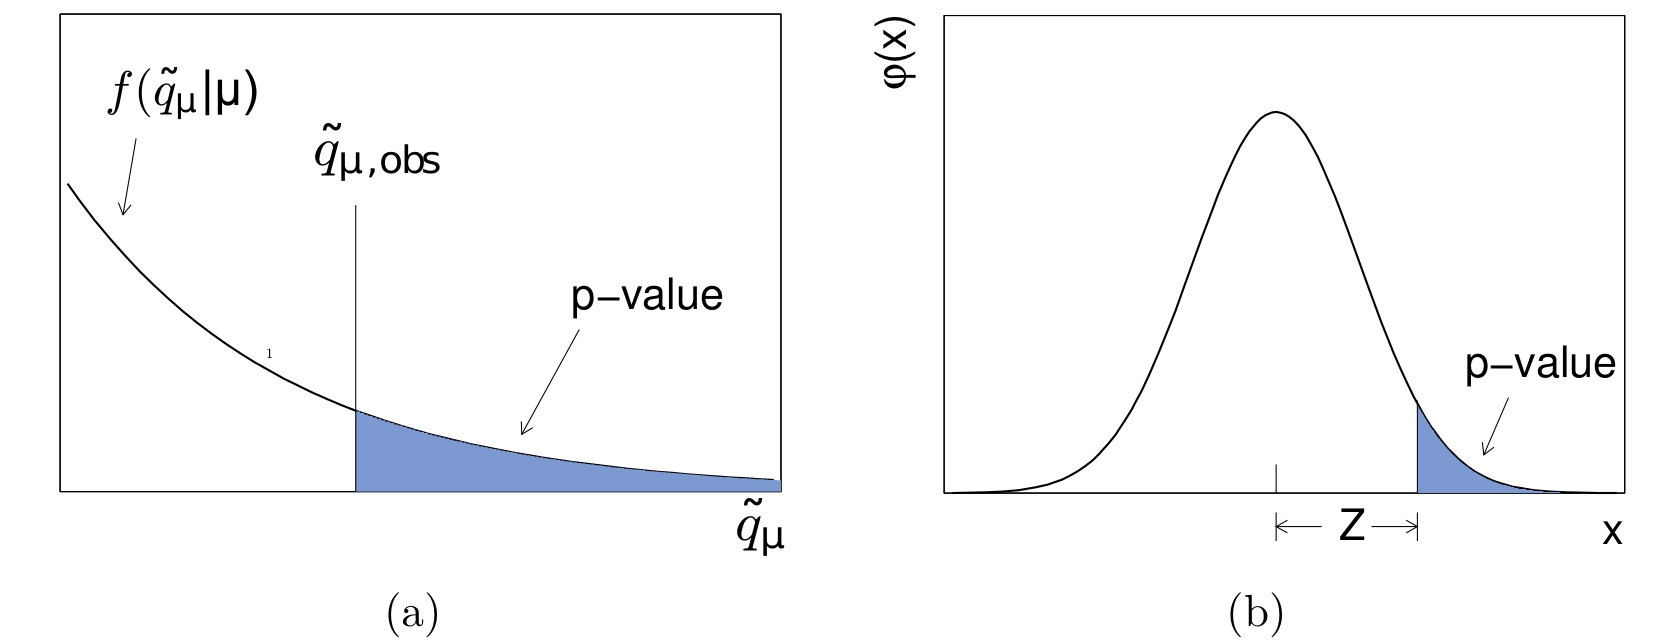
\includegraphics[scale=0.3]{images/4.jpg}
\caption{(a) p-value obtained using a test statistic $\hat{q}_{\mu}$. (b) Relationship between p-value and local significance Z as
derived from a standard Gaussian distribution $\phi(x)$ = $(1/ 2\sqrt{\pi})exp(-x ^{2}/2)$. Images adapted from \cite{<asym>}.}
\label{fig:asym}
\end{figure}
\section{Signal Strength Modifier of Higgs Signal}
Higgs-Signals are defined as the signal strengths at either a given mass peak or as functions of Higgs masses, considered as an observable in a computer code. The preliminary samples accumulated for Higgs-Signals via hadron colliders, are mainly by the LHC experiments, and is supported by the data from Tevatron. The Higgs-Signals methods have far reaching applications, for instance, data collection from a future $\eplus\eminus$ linear collider. 
This section will focus on the description of the experimental data that grants us the basic input for Higgs-Signals \cite{<ss1>}\cite{<ss2>}.\\
Explorations for Higgs bosons in CMS experiment are proceeded with the assumptions made in the Standard Model, such as Higgs-fermion couplings and Higgs-vector boson couplings, and both the cross sections and branching ratios are stated as a function of the Higgs boson mass, $m_{H}$. This gives permission for measuring one-parameter scaling e.g. $1\sigma$ of the total SM rate of a certain signal channel(s), supposedly signal strength modifiers, which come from best fitted data. They represent the basic observable input adopted in Higgs-Signals estimation. Samples from ATLAS and CMS are demonstrated in Fig.\ref{fig:sig1}.\\
\begin{figure}[h]
\centering
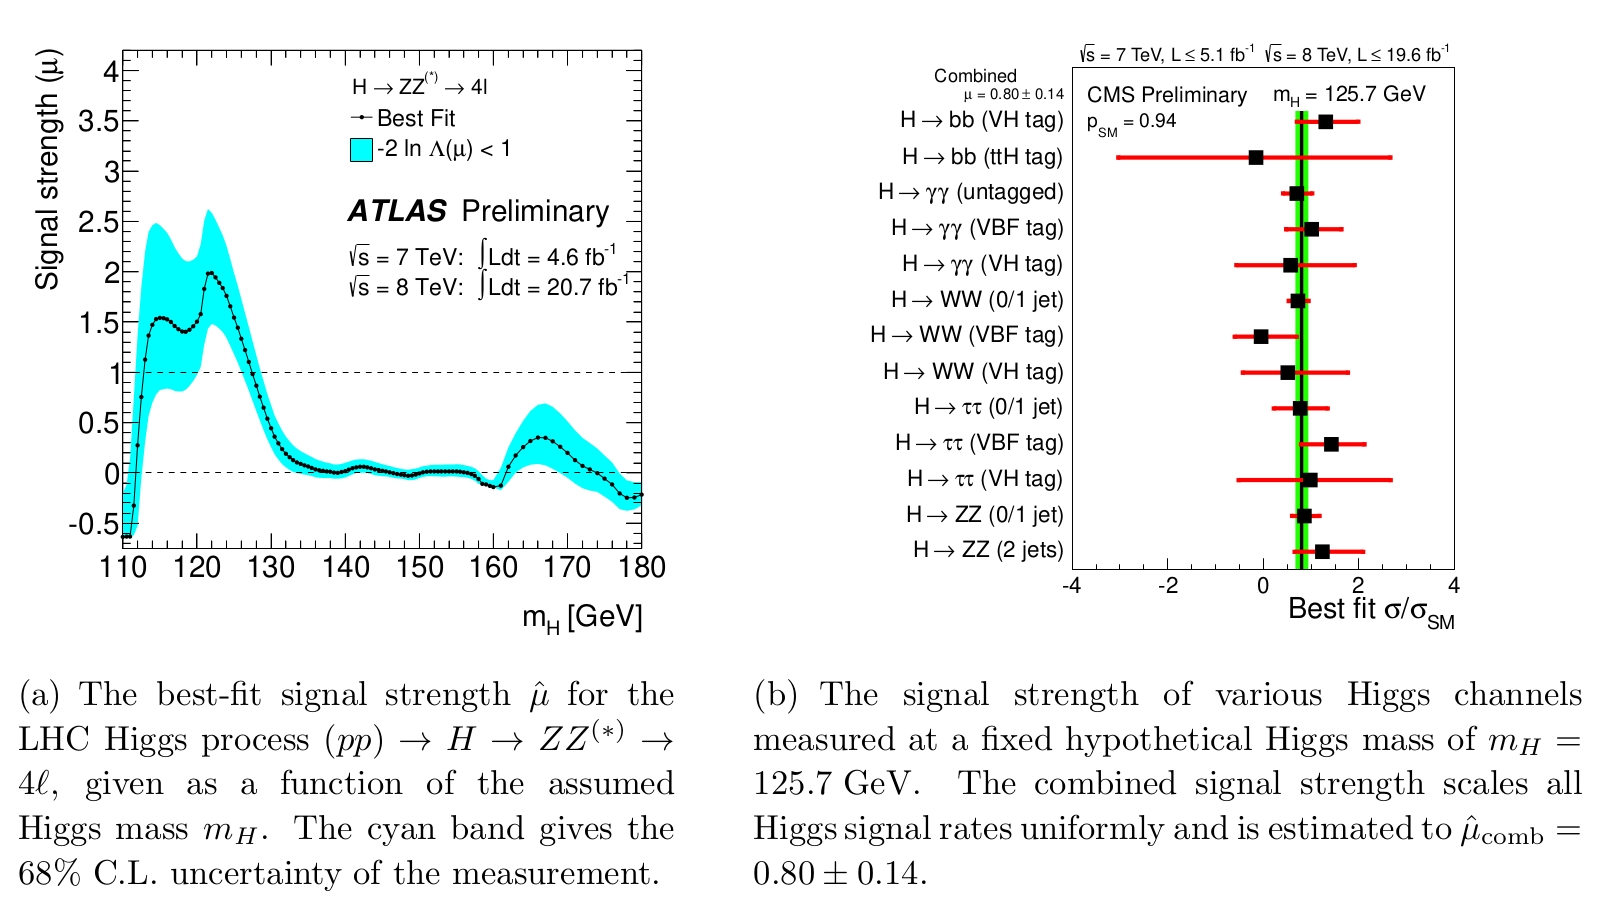
\includegraphics[scale=0.3]{images/signal1.jpg}
\caption{(a)signal strength modifiers by ATLAS \cite{<ss4>},
(b)the best fit rates according to CMS \cite{<ss3>}.}
\label{fig:sig1}
\end{figure}
The plot on the left (taken from \cite{<ss3>}) displays the measured signal strength modifier value, which is denoted by $\hat{\mu}$, in the interaction of $pp \rightarrow H\rightarrow ZZ^{\ast} \rightarrow 4l$ versus $m_H$ (black line) and an uncertainty $\pm1\sigma$ in measured rate is represented by the cyan band. Since the signal strength modifier illustrated in Fig.\ref{fig:sig1} (dashed line) is measured relative to its SM value ($\hat{\mu}$ = 1, it also encapsulates the theoretical uncertainties measured in branching ratios and cross section \cite{<ss4>}. The absence of signal-background interference in the signal model of SM never gives $\hat{\mu} < 0$, as seen in Fig.\ref{fig:sig1}, the measured value of $\hat{\mu}$ is permitted to have negative values. These negative values come from downwards statistical fluctuations in the data corresponding to the expected background value (the average expected background is $\hat{\mu}$ = 0).\\ 
To keep the authenticity intact, we retain full range of values of signal strength $\hat{\mu}$. In the following paragraph below we will see, the relevance of Higgs-Signals is restricted for range of masses in which the values $\hat{\mu}$ are detected. Hence accelerators should publish the mass regions where even SM Higgs signal are not measured.
The other example from CMS for Higgs-Signals input has been illustrated in the plot on right side of Fig.\ref{fig:sig1}(b) \cite{<ss4>}. Signal strength modifiers are summarized for Higgs decay modes at a value of $m_H$ = 125.7 GeV, where this value is commonly stated as it gives the maximum significance for a signal. It is essential to point out that when we fix a value for $m_H$, the plot also demonstrates different properties of various channels shown in Fig.\ref{fig:sig1}(b). Here, the horizontal error bars seen on $\hat{\mu}$ the measured values correlate the 1$\sigma$ uncertainties which are inclusive of SM, statistical and systematic uncertainties.\\
The Higgs-Signals matches the experimental signal strength modifier values with the predicted Higgs sector values in arbitrary models. The users give the predicted model for each parameter point to be tested over time known as simulations. We use five partonic subprocesses simulations for Higgs-Signals: gluon gluon fusion ($ggH$), vector boson fusion ($VBF$), vector boson associated production ($HW /HZ$), or top quark associated production ($ttH$) \cite{<ss5>}.\\
At base, Higgs-Signals runs on the LHC Higgs production cross sections and brancing ratios at centre-of-mass energy = 7 and 8 TeV as HiggsBounds-4, a tool which tests models of Higgs sectors having neutral and charged Higgs bosons, \cite{<ss3>}\cite{<ss5>}\cite{<ss6>}\cite{<ss7>}.\\
According to the theory, if signal strength modifier is predicted from one Higgs boson H, it is programmed in Higgs-Signals as
\begin{equation}
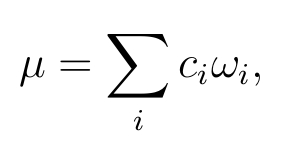
\includegraphics[scale=0.3]{images/hs1.jpg}
\end{equation}
here summation is over all the analysis channels used. A particular channel is specified by a distinct production and a distinct decay mode. Signal strength of a particular channel is defined as
\begin{equation}
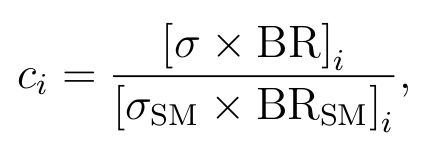
\includegraphics[scale=0.3]{images/hs2.jpg}
\end{equation}
and the SM channel weight as
\begin{equation}
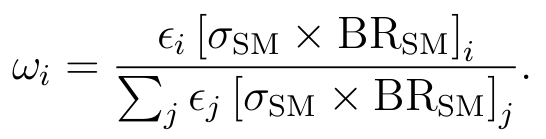
\includegraphics[scale=0.3]{images/hs3.jpg}
\end{equation}
The SM weights include the corresponding efficiencies, $\epsilon_{i}$ from the experiment, for the specific channels. If they are mentioned in experimental publications, we can use these numbers for Higgs-Signals, and have reliable comparison between the experimental data  and theory for specific channels. Where the efficiencies for channels are not known, all values are set to $\epsilon_{i}\equiv1$. Although many a times observable's close values for the channel efficiencies are calculated by reconstruction of fit results on scale factors of cross sections or coupling strengths in production.
As a caution it must be noted; if the model contains a non-standard tensor structure for the particles to be measured, which can be figured out from the data, the processes might include notable discrepancies in the kinematic distributions measured experimentally and in turn violate the signal efficiency acceptance in the data analyses of Higgs.
\section{Event Categorization}
\label{section:ec}
For the optimization of production modes of Higgs boson, signal events are divided into specific event categories. Categories are divided using observables typically from supplementary objects in the event, which have different sensitivity for different production modes. In Run I of LHC, two categories were defined using observed number of jets in an interaction, where fermion-Higgs and $V B \PHiggs$ couplings could already be measured. Run II of LHC had a more diversified categorization, which targets five main production mechanisms. Chosen signal events are divided into mutually exclusive event categories, each of which dominates a production mode.\\
This section will briefly review observable used in the categorization before stating the categorizations for 2016, 2017 and 2018 analysis, respectively.\\

\textbf{Categorizing Objects}\\
To acquire information about Higgs boson production mechanisms, apart from the four selected leptons, additional objects in the detector during each interaction are considered. Additional leptons which we describe as leptons that are not involved in selected $ZZ$ candidates and selected jets are taken into account. Event categorization has two types of input as observable: one which counts the number of additional objects in the event and the other which is the matrix-element based production discriminant based on jet kinematics and leptons.
\begin{enumerate}
    \item Selected jets number, for specific production mechanism such as $VBF, VH$ (1-2 jets in the event), and $\Ptop \Bar{\Ptop}\PHiggs$ (3 or more jets as in the event),
    \item Selected b-tagged jets number, which focuses on $ZH$ with $\PZ \rightarrow \Pqb \Paqb$ and $\Ptop \Bar{\Ptop}\PHiggs$,
    \item Additional leptons number, aiming at $\Ptop \Bar{\Ptop}\PHiggs\PHiggs$ and leptonic VH events,
    \item Opposite-sign same-flavour leptons pair number, which are unique for leptonic $\Ptop \Bar{\Ptop}\PHiggs$ and leptonic $ZH$ events.
    \item The observable which targets $VH$ events with neutrinos as decay products.
    \item Also the observable that counts the object numbers in an event, observable with neutrinos sensitivity and missing transverse momentum $E^{miss}_T$. 
\end{enumerate}

\subsection{2016 Data Categorization}
If an event does not fulfil requirements of selection for a particular category, it is considered for the subsequent category. In 2016 data accumulation at CMS experiment seven categories were selected:
\begin{SCfigure}
\centering
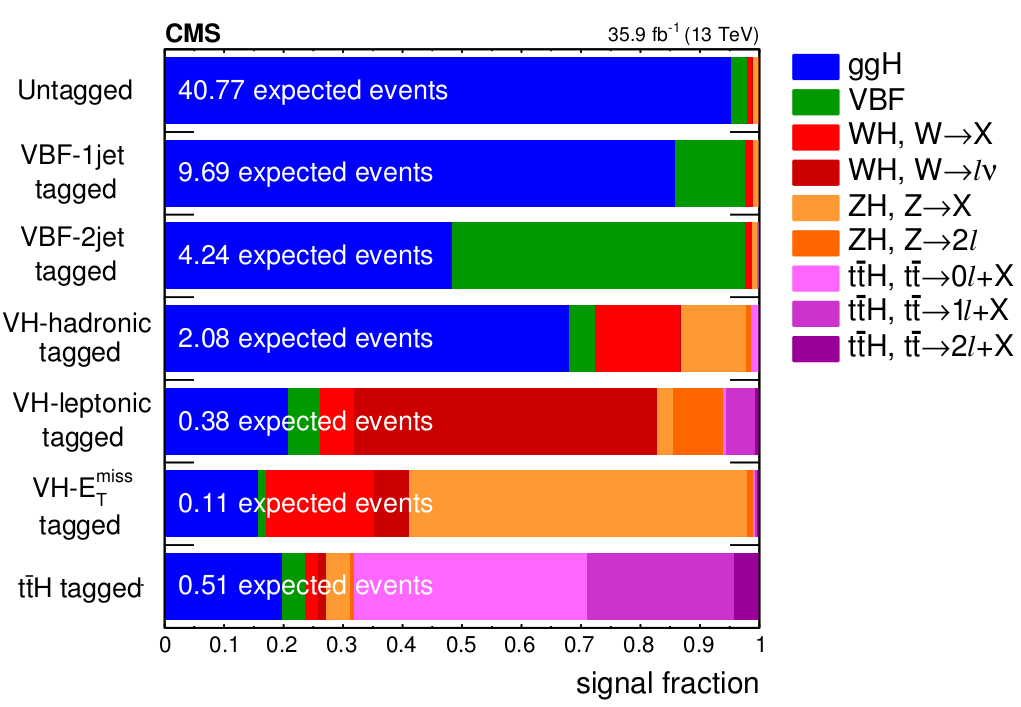
\includegraphics[scale=0.25]{images/cat1.png}
\caption{Composition of the categories in 2016 analysis in the $118 < m_{4l} < 130$ GeV window. The symbol X is for particles other than electrons muons.  \cite{<thesis>}.}
\label{fig:cat1}
\end{SCfigure}
\begin{itemize}
    \item \textbf{2jet-VBF} which has 4 leptons. 2-3 jets where one is b-tagged at the most, or (4 or more) not b-tagged jets. $D^{ME}_{VBF - 2j}> 0.5$.
    \item \textbf{hadraonic-VH} which has 4 leptons. 2-3 jets where one is b-tagged at the most, or (4 or more) not b-tagged jets. $D^{ME}_{VH} \equiv max(D^{ME}_{ZH}, D^{ME}_{WH}) > 0.5$.
    \item \textbf{leptonic-VH} should have 3 jets at minimum, exactly 1 additional lepton , 1 additional pair of OS, same-flavor leptons and no b-tagged jets. It can also contain events with at minimum 1 additional lepton and zero jets.
    \item \textbf{$\Ptop \Bar{\Ptop}\PHiggs$} should have at minimum 4 jets in which at minimum 1 is b-tagged, or at minimum 1 additional lepton.
    \item \textbf{$E^{miss}_{T}$-VH} should have 4 leptons, at most 1 jet and $E_{T}^{miss}$ greater than 100 GeV.
    \item \textbf{1jet-VBF} should have 4 leptons, exactly 1 jet and $D^{ME}_{VBF - 1j} > 0.5$.
    \item The \textbf{Untagged} entails the rest of selected events.
\end{itemize}
\vspace{4mm}
\subsection{2017 Data Categorization}
The 2017 data analysis was to be preliminary done by promptly reproduced data and the $E^{miss}_{T}-VH$-tagged category was dropped and another one in its place was adopted for the 2017 event categorization. The following seven categories are considered:
\begin{itemize}
      \item \textbf{2jet-VBF} which has 4 leptons. 2-3 jets where one is b-tagged at the most, or (4 or more) not b-tagged jets. $D^{ME}_{VBF - 2j}> 0.5$.
    \item \textbf{hadraonic-VH} which has 4 leptons. 2-3 jets where one is b-tagged at the most, or (4 or more) not b-tagged jets. $D^{ME}_{VH} \equiv max(D^{ME}_{ZH}, D^{ME}_{WH}) > 0.5$.
    \item \textbf{leptonic-VH} should have 3 jets at minimum, exactly one additional lepton , one additional pair of OS, same-flavor leptons and no b-tagged jets. It can also contain events with at minimum 1 additional lepton and zero jets.
    \item The \textbf{hadronic-$\Pqt\Paqt\PHiggs$} should have 4 jets at minimum, of which at least 1 is b-tagged and there are no additional leptons.
    \item The \textbf{leptonic-$\Pqt\Paqt\PHiggs$} should have 1 additional lepton.
     \item \textbf{1jet-VBF} should have 4 leptons, exactly 1 jet and $D^{ME}_{VBF - 1j} > 0.5$.
    \item The \textbf{Untagged} entails the rest of selected events.
\end{itemize}
\begin{figure}[h]
\centering
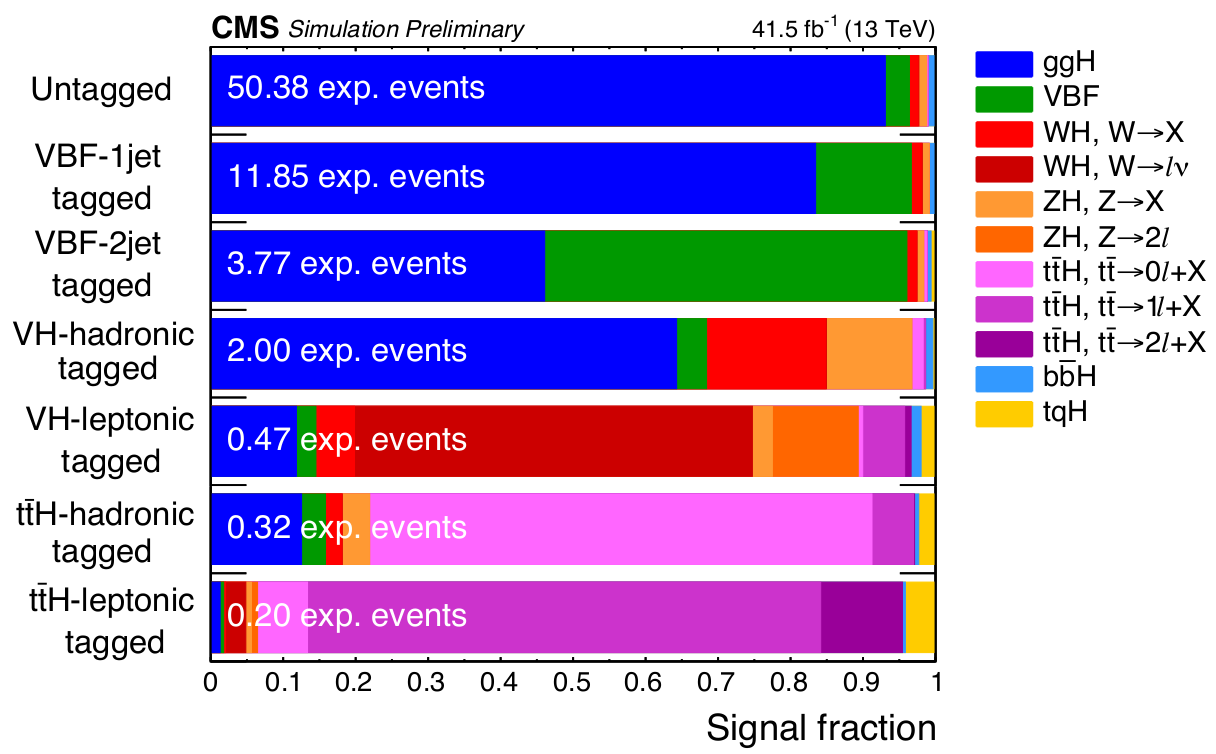
\includegraphics[scale=0.25]{images/cat2.png}
\caption{Event categories of the 2017 data analysis in the $118 < m_{4l} < 130$ GeV window. The X symbol stands for particles other than electrons muons.\cite{<thesis>}}
\label{fig:cat2}
\end{figure}

\subsection{2018 Data Categorization}
In 2018 categorization a VH-MET Category is added along with 2017 reconstructed events and categories are further split into sub categories.
\begin{itemize}
    \item The \textbf{VH-MET} requires one missing lepton at the vmost, no more than 1 jet and and missing transverse momentum $E^{miss}_{T}> 100$ GeV.
\end{itemize}
Reconstructed events are further subdivided in the next step of the categorization, the Untagged,  VBF-2jet, VH-leptonic, and VH-hadronic categories are then divided further, exploiting additional variables e.g. the transverse momentum of the ZZ candidate and the invariant mass of the two leading jets as illustrated in Fig.\ref{fig:cat3}. The number of event categories used each year corresponding to their integrated luminosity are mentioned in Table.\ref{tab:dat}.

\begin{figure}
\centering
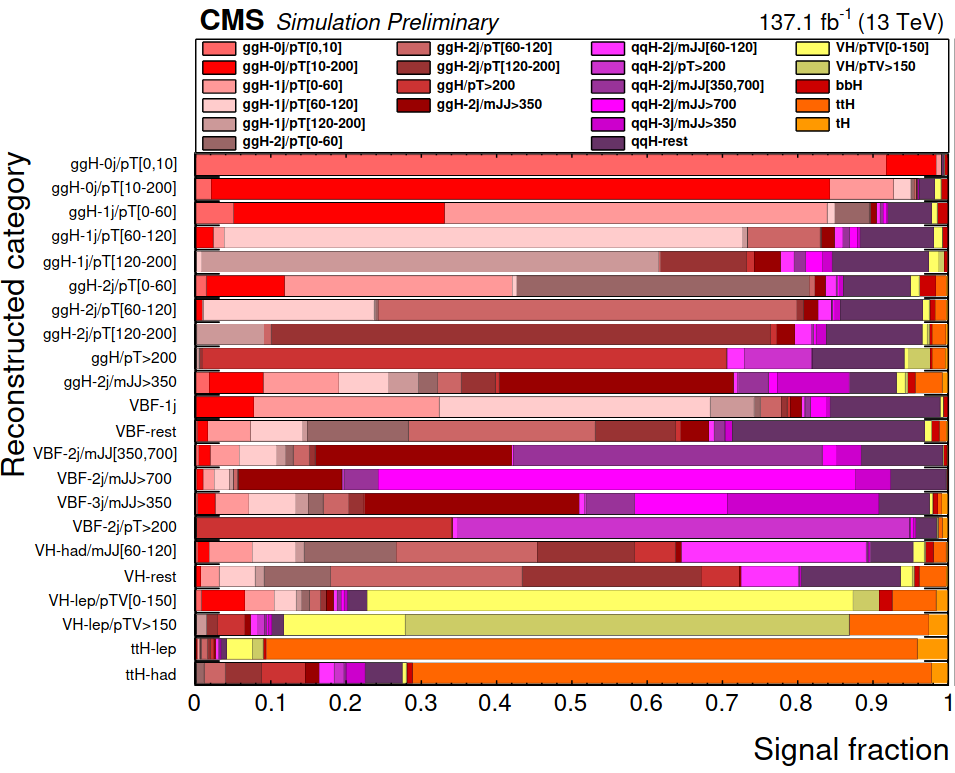
\includegraphics[scale=0.26]{images/cat3.png}
\caption{Distributions after event reconstruction for the mass range $105 < m_{4l} <140$ GeV in year 2018.\cite{<2021>}}
\label{fig:cat3}
\end{figure}
\begin{table}[]
    \centering
    \begin{tabular}{|c|c|c|}
    \hline
       Data Year  & Integrated Luminosity & Event Categories \\
      \hline
      2016 & 35.9 fb$^{-1}$ & 6 \\
    2017 & 41.5 fb$^{-1}$ & 7 \\
    2018 & 59.7 fb$^{-1}$ & 8 \\
    \hline
    \end{tabular}
    \caption{Analysis Factors}
    \label{tab:dat}
\end{table}


\section{Analytical Techniques}
After defining $H \rightarrow ZZ^* \rightarrow 4l$ analysis building blocks (event categories), the most integral part is to verify how the final measurements are in accord with the simulations. During the Run I of LHC, the search for Higgs boson was at forefront, by searching for specific events in an unlimited amount of events in accordance with the Standard Model prediction and organizing it. The Run II shifted the focus to property measurements of Higgs and in looking for new physics. For modelling different properties, different statistical methods are used, and this section will introduce the statistical distributions used for model fitting.
\subsection{Gaussian Distribution}
\label{section:gd}
The Gaussian (Normal) PDF of $x$, a continuous random variable with $- \infty < x < \infty$ is described as,
\begin{equation}
    f (x; \mu \sigma^2) = \frac{1}{2 \pi \sigma^2} exp \left ( \frac{-(x-\mu)^2}{2 \sigma^2} \right),
\end{equation}
where $\mu$ is the mean and $\sigma^2$ is the variance of Gaussian distribution. They are given as,
\begin{equation}
    \begin{aligned}
        &E[x] = \int ^{\infty}_{- \infty} x \frac{1}{2 \pi \sigma^2} exp \left ( \frac{-(x-\mu)^2}{2 \sigma^2} \right)dx = \mu, \\
        &V[x] = \int ^{\infty}_{- \infty} (x-\mu)^2 \frac{1}{2 \pi \sigma^2} exp \left ( \frac{-(x-\mu)^2}{2 \sigma^2} \right)dx = \sigma^2
    \end{aligned}
\end{equation}
$E[x]$ gives a range of values where $x$ are likely to be detected. For instance, the $f(x)$ might show two widely separated peaks, where $E[x]$ is in the middle and $x$ occasionally (or is never) observed. The variance $V[x]$ represents the spread in data given by $x$, around the mean value.
\begin{figure}[h]
\centering
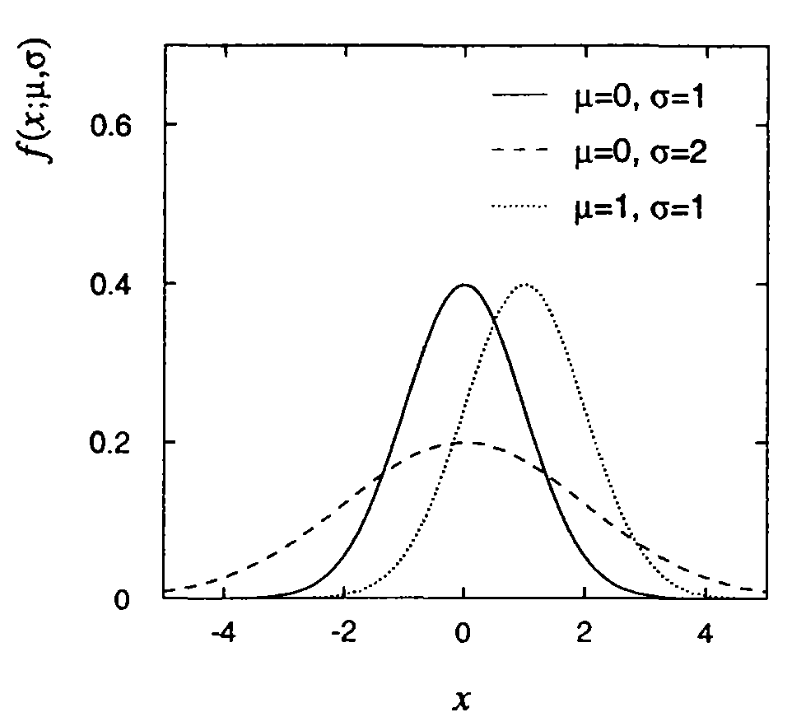
\includegraphics[width=0.3\textwidth]{images/var.png}
\caption{The Gaussian PDF for various values of the parameters $\mu$ and               $\sigma$.}
\label{fig:var}
\end{figure}
In a particular case, the standard Gaussian $\phi(x)$ (with $\mu = 0$ and $\sigma=1$ is defined as such, 
\begin{equation}
    \phi(x) = \frac{1}{\sqrt{2 \pi}} exp ( - x^2/2), 
\end{equation}
with $\Phi(x)$ as corresponding distribution.
\begin{equation}
    \Phi(x) = \int ^x_{- \infty} \phi(x)' dx'.
\end{equation}
To check if $y$ is distributed according to a Gaussian PDF, then
\begin{equation}
x= \frac{y-\mu}{\sigma}
\end{equation}
here the cumulative distributions are correlated by $F(y) = \Phi(x)$. There is no analytical representation of cumulative distribution, so we have to perform numerical evaluation. Values of $\Phi(x)$ along with $x_0 = \Phi(x)^{-1}(\alpha)$ are tabulated in reference books \cite{<gd1>,<gd2>,<gd3>,<gd4>} and instilled in computer program libraries, e.g. the routines FREQ and GAUSIN \cite{<gd5>}. The central limit theorem gives significance to Gaussian distributions. The theorem states that the sum of n random continuous independent variables $x_i$ having mean value $\mu_i$ with variance $\sigma_i$ becomes a Gaussian random variable when the limit n approaches to infinity, having mean value $\mu = \sum^n _{i=1} \mu_i$ and variance $\sigma^2 = \sum^n _{i=1} \sigma_i^2$. This provides measurement errors with Gaussian random variables treatment, and is extended till the total error becomes the sum of unlimited values giving small contributions from each variable.\\
The N-dimensional generalization of the Gaussian distribution is  defined by 
\begin{equation}
    f(x; u,V) = \frac{1}{(2 \pi)^{N/2}|V|^{1/2}}exp \left[- \frac{1}{2}(x-\mu)^T V^{-1}(x-\mu)\right],
\end{equation}
here column vectors are given by $x$ and $\mu$, and row vectors by $x^T$ and $\mu^T$ and $|V|$ represents the determinant of a symmetric $N \times N$ matrix $V$, with free parameters amounting to $N (N + 1) /2$. The (co)variances and expectation values are;
\begin{equation}
    \begin{aligned}
        E[x_i]=\mu_i\\
        V[x_i]=V_{ii}\\
        cov[x_i, x_j]=V_{ij}.
    \end{aligned}
\end{equation}
\subsection{Landau Distribution}
\label{section:ld}
In nuclear and particle physics there is mostly energy loss $\triangle$ when a charged particle travels through a layer of matter with a known thickness, which is given with the probability density $f (\triangle;\beta)$. Landau \cite{<LD>}, was the first one to derive this probability density given by,
\begin{equation}
    f(\triangle;\beta) = \frac{1}{\xi} \phi (\lambda), \hspace{3mm} 0 \leq \triangle < \infty,
\end{equation}
here the parameter $\xi$ and $\lambda$ relate to the property of the material, $\beta = v/c$ to the velocity of the particle, and $\phi (\lambda)$ is the PDF of the dimensionless random variable $\lambda$. These quantities are given by
\begin{equation}
    \begin{aligned}
    &\xi = \frac{2 \pi N_A e^4 z^2 \rho \sum Z}{m_e c^2 \sum A}\frac{d}{\beta^2},\\
    & \lambda = \frac{1}{\xi} \left [\triangle - \xi \left(log \frac{\xi}{\epsilon'}+1- \gamma_E \right) \right],\\
    &\epsilon' = \frac{I^2 exp (\beta^2)}{2 m_e c^2 \beta^2 \gamma^2},
    \end{aligned}
\end{equation}

where $N_A$ is the Avagadaro's number, $m$, $e$ are mass and charge of the electron, $z$ is incident particle's charge, $\sum Z, \sum A$, gives summation over the atomic number and atomic weights of the molecular substance, $\rho$ is density, $d$ is thickness, $I=I_0 Z$ where $I_0$ = 13.5eV is the ionization characterisation of the material, $\gamma = \sqrt{1-1/\beta^2}$, and Euler's constant $\gamma_E = 0.5772 \cdots$. The function: 
\begin{equation}
\begin{aligned}
    &\phi(\lambda)= \frac{1}{2 \pi i} \int^{\epsilon + i \infty}_{\epsilon - i \infty} exp(u log u + \lambda u)du,\\
    &\phi(\lambda)= \frac{1}{\pi} \int^{\infty}_{0} exp(- u log u + \lambda u) sin \pi u du,
    \end{aligned}
\end{equation}
\begin{figure}[h]
     \centering
     \begin{subfigure}[b]{0.45\textwidth}
         \centering
         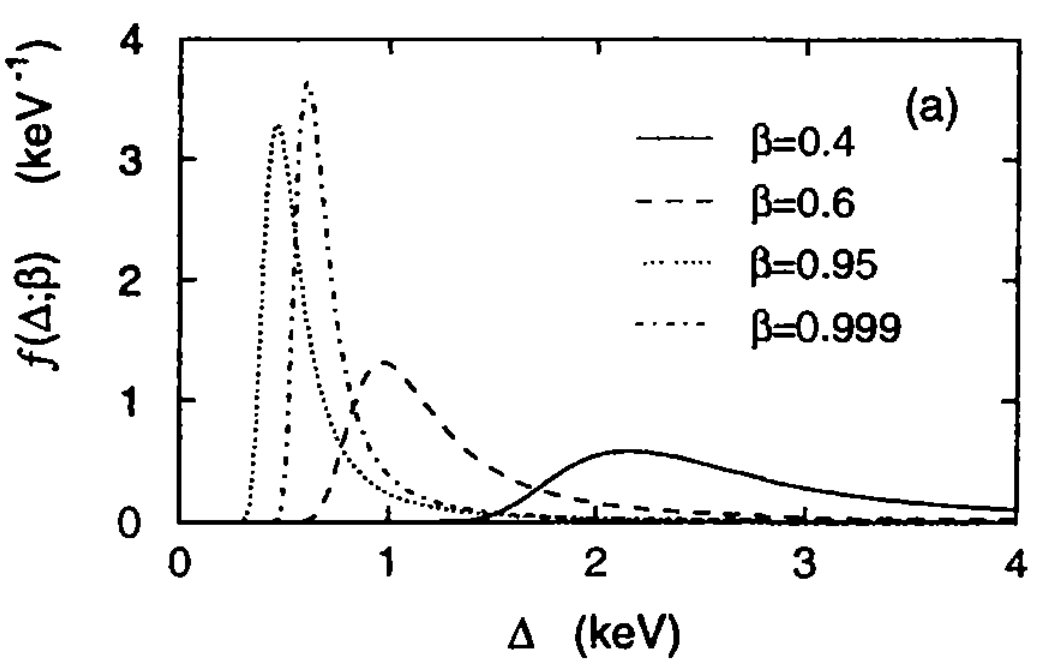
\includegraphics[width=\textwidth]{images/LD2.png}
     \end{subfigure}
     \hfill
     \begin{subfigure}[b]{0.45\textwidth}
         \centering
         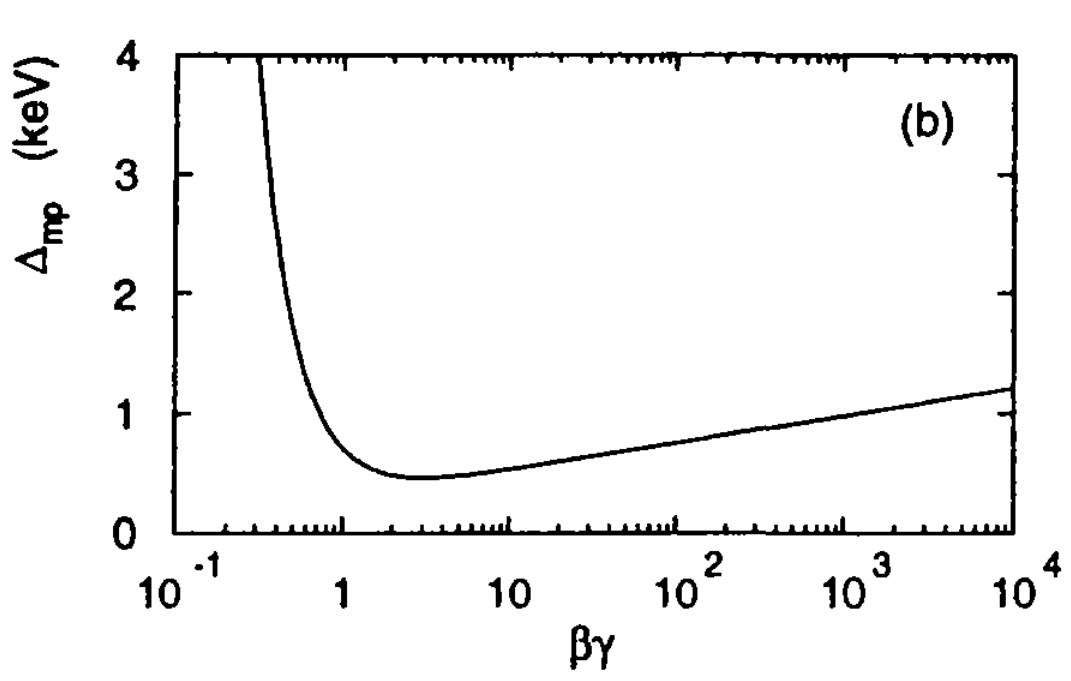
\includegraphics[width=\textwidth]{images/LD.png}
     \end{subfigure}
     \hfill
        \caption{(a)The Landau probability density with energy loss $\triangle$ of a charged particle travelling through a 4 mm thick layer of argon gas at stp at different values of the velocity $\beta$. (b)The peak modes in (a) as a function of $\beta_\gamma$ from Eq.3.14}
        \label{fig:LD}
\end{figure}
The distribution of energy loss is demonstrated in Fig.\ref{fig:LD}(a) for different $\beta$ values. There are no mean and higher moments of the Landau distribution because of long tail extending to high values of $\triangle$, i.e. the integral $\int^{\infty}_{0} \triangle^n f(\triangle) d\triangle$ diverges for $n\ge1$. The Fig.\ref{fig:LD}(b) demonstrates that the common mode $\triangle_{mp}$ is sensitive to the particle's velocity which was numerically computed \cite{<mac69>} to be, 
\begin{equation}
    \triangle_{mp} = \xi [log(\xi/\epsilon')+0.198],
\end{equation} 
The `Bethe-Bloch formula' as the above equation is popularly known as and given in books e.g. Subatomic Physics by Henley \cite{<sap>}, is basis on which charged particles are identified by measurement of ionization energy loss \cite{<bbf>}.\\
As for Landau, the mean and higher moments do not exist for the Breit-Wigner distributions, this is due to the fact that probability densities which are used to describe physical processes require finite moments. When measuring energy loss $\triangle$ of a particle repetitively, the average would converge to some value, as energy loss can never be higher than the energy of the incoming particle. Same is the case for the mass of a resonance particle, it should never be less than the sum of the rest masses of corresponding decay products, and higher than the center-of-mass energy of the reaction where it occurred. This creates a problem when the Cauchy and Landau distributions are approximating models of physical system but break down at the tails, which in the PDF causes the mean and higher moments to diverge \cite{<cowan>}.
\subsection{Breit-Wigner Distribution}
\label{section:bwd}
The Cauchy or Breit-Wigner probability density function of the continuous variable $x$ $(- \infty < x < \infty)$ is defined as, 
\begin{equation}
    f(x) = \frac{1}{\pi} \cdot \frac{1}{1 + x^2}.
\end{equation}
Given below is a special case of the Breit-Wigner distribution we see in particle physics,
\begin{equation}
    f (x; \Gamma, x_0) = \frac{1}{\pi} \frac{\Gamma/2}{\Gamma^2 /4  + (x- x_0)^2},
\end{equation}
where the mass is given as $x_0$ and width as $\Gamma$ of a resonance particle as illustrated in Fig.\ref{fig:bw}; $x_{0}$ represents the peak mode and $\Gamma$ represents the full-width of the peak at half of the maximum height \cite{<gd3>,<bwd>}.\\
\begin{SCfigure}[][h]
    \centering
    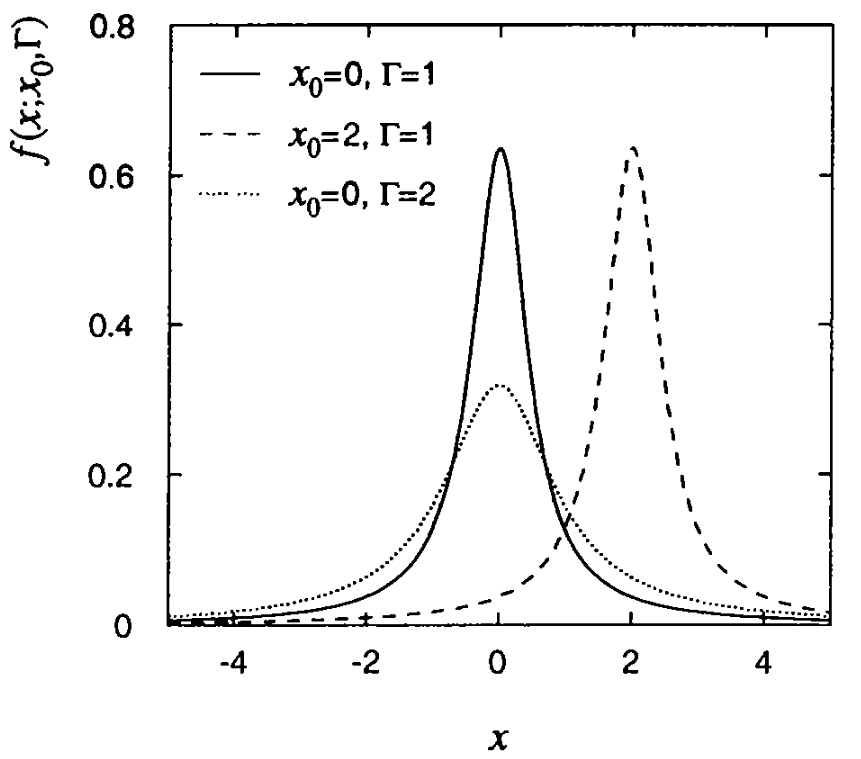
\includegraphics[scale=0.2]{images/bw.png}
    \caption{The Cauchy (Breit-Wigner) PDF for different values of the parameters $x_0$ and $\Gamma$.}
    \label{fig:bw}
\end{SCfigure}
The Cauchy distribution does not have well defined expectation value, even with a symmetric PDF about zero (or $x_0$ for Eq.3.8). The integrals $\int^{0}_{-\infty} xf(x)dx$ and $\int^{\infty}_{0} xf(x)dx$ diverge separately on their own, along with variance and higher moments \cite{<cowan>}. The Cauchy distribution is a normal ratio distribution, a ratio of two normalised distributions with mean zero. For two random variables $p$ and $q$, the ratio distribution of a third random variable $w$ is defined as $w = p/q$. 
\subsection{Double Shouldered Crystal Ball Function}
\label{section:dcb}
The Crystal Ball function, named after the Crystal Ball (hermetic particle detector), is a PDF typically used when modelling various particle physics processes which have energy losses. It contains a Gaussian core portion shown in Fig.\ref{fig:gbw} and below a distinct threshold a power law end tail shown in Fig.\ref{fig:CBF}. It is a continuous function with continuous first derivatives. A Double Crystal Ball (DCB) Function has two power-law end-tails on both sides:
\begin{figure}[h]
    \centering
    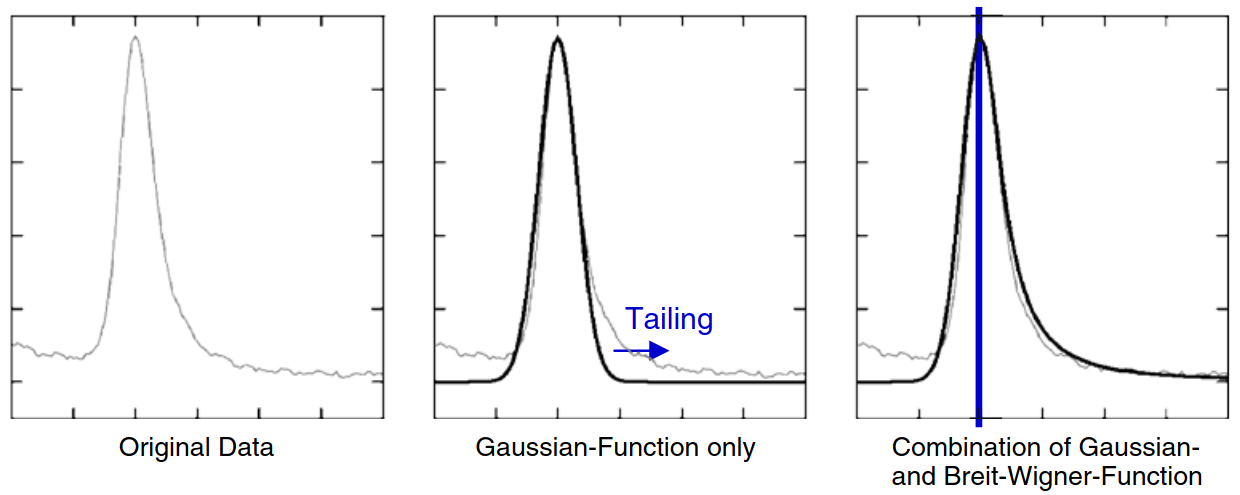
\includegraphics[scale=0.3]{images/gbw.png}
    \caption{A single spectrum of data, the application of the Gaussian function with a tail and the combination of Gaussian and Breit-Wigner-Function for best fit.}
    \label{fig:gbw}
\end{figure}
\begin{equation}
    dCB(\epsilon) = N \cdot 
    \left \{\begin{aligned} & D_1. (D_2 + |\epsilon|)^{-n_L}, \hspace{2mm} \epsilon < \alpha_L \\ &D_1 . (D_2+ |\epsilon|)^{-n_R}, \hspace{2mm} \epsilon > \alpha_R \\ &exp(- \epsilon^2/2),\hspace{1mm} \alpha_L \leq \epsilon \leq \alpha_R  \end{aligned} \right \} 
    \label{eqn:dcb}
\end{equation}
here $\epsilon = (m_{4l} - m_H - \triangle m_H )/ \sigma_m$. DCB with 6 independent parameters, captures the Gaussian core $(\sigma_m)$ of mass resolution function of the four leptons and $\triangle m_H$ mass shift of the peak, and the left- and right-hand tails originating from tracker bremsstrahlung emitted by leptons, which exist for both electrons and muons, and from the non-Gaussian mis-measurements which are unique for events of electrons with the experimental material. The effectiveness of the side tails is shown by the power $n_L , n_R$, respectively. Here parameters $\alpha_L , \alpha_R$ define slicing of the tails and $\sigma_m$ defines the core. Parameters $D_1$ and $D_2$ are not independent; they are described by function continuity along with it's first derivatives. N is the normalizing constant.\cite{<toni>}
\begin{figure}
    \centering
    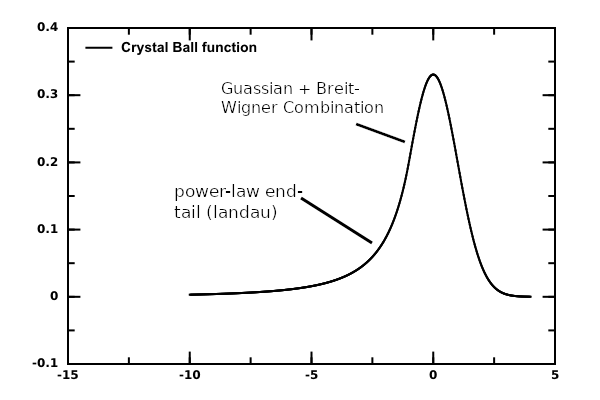
\includegraphics[scale=0.4]{images/CBF.png}
    \caption{Double Crystal Ball Function}
    \label{fig:CBF} 
\end{figure}
\subsection{Pull Distribution}
\label{section:pd}
The pull of a bin is defined as the difference between model function and value of the histogram, divided by the error of the histogram value $(\frac{residue}{error})$. If the model describes the histogram, the pulls should be distributed as a normal distribution with a width of 1 centered around the origin, i.e. plot of the distribution $\Phi_i$ should be a Gaussian, centered at 0, and width=1.
\begin{figure}[h]
    \centering
    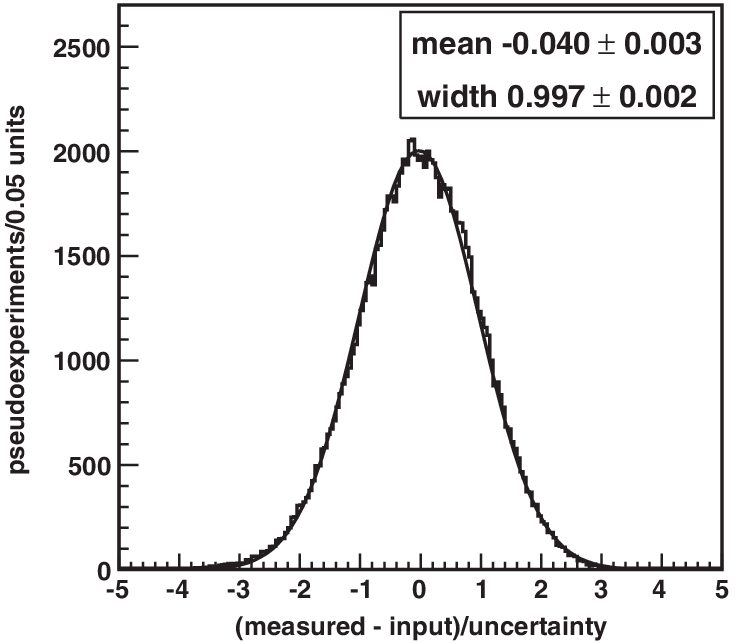
\includegraphics[scale=0.25]{images/pd.png}
    \caption{Pull distribution from pseudo-experiments run with the likelihood used to find the combined cross section \cite{<pd2>}.}
    \label{fig:pd}
\end{figure}
This controls the quality of the fit. If this test fails, we say that the used model does not match the experimental measurements, the measurements used for the weights are biased or error estimates are not properly estimated \cite{<pd1>}. Pull or stretch values of fitted parameter $i$ is defined as
\begin{equation}
    \triangle_i = (x_i - \mu)/ \sigma_i
\end{equation}
An example of pull distribution is given in Fig.\ref{fig:pd}. Some properties taken into account while plotting a pull are:
\begin{itemize}
    \item If not centered in $0 \rightarrow$ bias in measurement,
    \item If pull width $ < 1$, uncertainty is under-covered,
    \item If pull width $ > 1$, uncertainty is overestimated. 
\end{itemize}

\subsection{Chebyshev Polynomials}
\label{section:cp}
This relates to deriving a simple polynomial function $f(x)$ to fit to a given function  $g(x)$, that can be used to approximate the original function. This is especially useful when the original function is difficult to differentiate or integrate.
\clearpage
\textbf{Chebyshev Theorem}\\
\begin{wrapfigure}[]{l}{0.4\textwidth}
\vspace{-30pt}
\begin{center}
    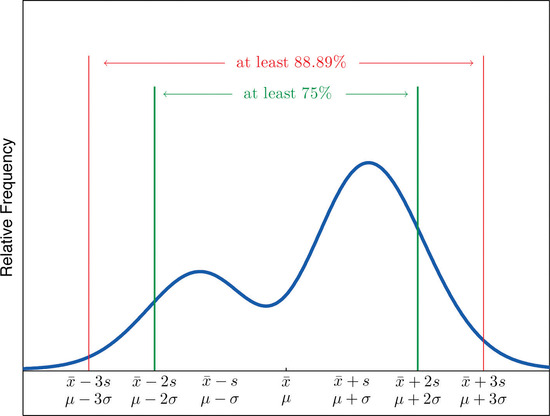
\includegraphics[scale=1]{images/CT.jpg}
\end{center}
\vspace{-20pt}
\caption{Chebyshev's Theorem \cite{<cheb1>}}
    \label{fig:ct}
    \end{wrapfigure}
    For any numerical data set as shown in Fig.\ref{fig:ct}:\\
\begin{enumerate}
    \item at least $1 - 1/\kappa^{2}$ events are inside $\kappa$ standard deviations of the mean, i.e. endpoints $\bar{x} \pm \kappa s $ for samples and endpoints $\mu \pm \kappa \sigma$ for populations where $\kappa > 1 $;
\end{enumerate}
For values only in $\xi \hspace{2mm} \epsilon \hspace{2mm}[1,-1]$ interval, the $x^{th}$ \textbf{Chebyshev's Polynomial} $T_x (\xi)$ is described as,
\begin{equation}
    T_x (\xi) \equiv cos (x\cdot arccos(\xi)), x=1,2, \cdots.
\end{equation}
This describes the function domain $arccos(x)$. First we consider the first three Chebyshev's polynomial and check if they are indeed polynomials;
\begin{equation}
    \begin{split}
        &T_I (\xi) = cos (0 arccos(\xi))=1,\\
        &T_{II} (\xi) = cos (1 arccos(\xi))=\xi,\\
        &T_{III} (\xi) = cos (2 arccos(\xi))=2 [cos(arccos(\xi))]^{2}-1=2 \xi^2 - 1,
    \end{split}
\end{equation}
Using the formula for double angle, $cos2\theta = 2 \cdot cos^2 \theta - 1$ to derive $T_{II}(\xi)$ and $cos(\alpha)+cos(\beta)= 2 cos(\frac{\alpha+\beta}{2})+cos(\frac{\alpha-\beta}{2})$ we derive the higher order polynomials. i.e.
\begin{equation}
    \begin{split}
        &\hspace{-15mm}T_{x+1}(\xi)+T_{x−1}(\xi)=cos[(x + 1)arccos(\xi)]+cos[(x−1)arccos(\xi)]\\
        & = cos [x\cdot arccos(\xi) + arccos(\xi)] + cos[x\cdot arccos(\xi) - arccos(\xi)]\\
        & =2 cos[x\cdot arccos(\xi)] cos [arccos(\xi)]\\
        & =2\xi T_x (\xi).
    \end{split}
\end{equation}
The Chebyshev polynomials uses recurrence relation,
\begin{equation}
    T_{x+1}(\xi) = 2\xi T_x(\xi) - T_{x - 1}(\xi), \hspace{2mm}  x=1,2, \cdots.
\end{equation}
This method shows that if we have a N degree Chebyshev's polynomial $T_N (x)$, $x$ has even(odd) powers corresponding to if N is even(odd). The first eighth terms in power series form and in Chebyshev's series form, are displayed in Table.\ref{tab:cp}.
\begin{table}
    \centering
    \begin{tabular}{c}
       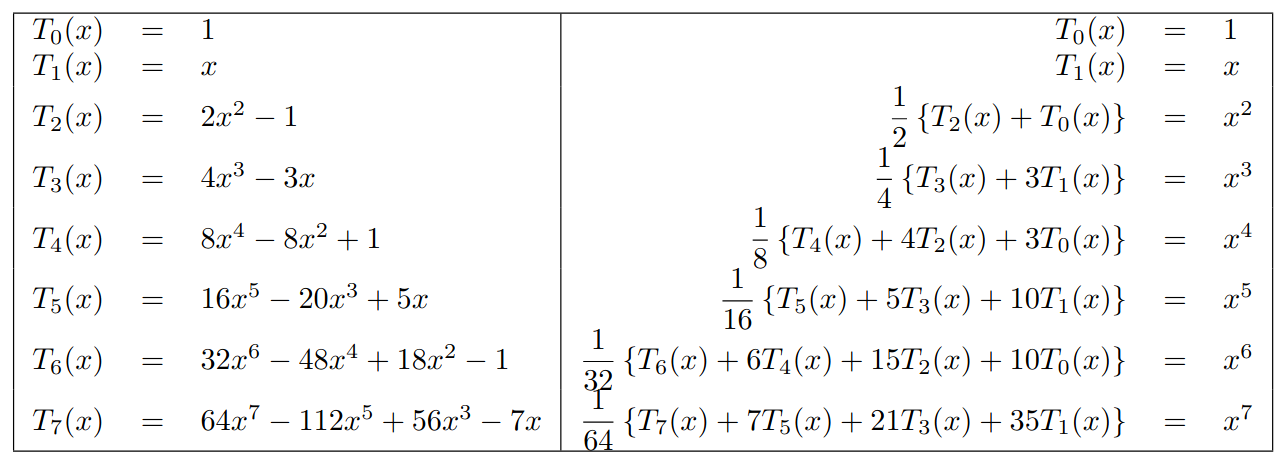
\includegraphics[scale=0.3]{images/cheb1.png} 
    \end{tabular}
    \caption{Chebyshev's Polynomial Conversion Table}
    \label{tab:cp}
\end{table}
The advantage of choosing Chebyshev's polynomial, shown in Fig.\ref{fig:cp2} $T_x(\xi)=cos(x arccos(\xi))$ as opposed to the power term $\xi^x$ for showcasing data for values $\xi_\epsilon$ $[ - 1,+ 1]$ is that $T_x(\xi)$ oscillates x number of times in between $\xi=-1$ and $\xi= + 1$. Also, with the increase in x value the end zero crossings on both side of data for $T_x(\xi)$ almost nears, but never cross, the range endpoints $\xi =-1$ and  $\xi = + 1$. Hence, the polynomials of Chebyshev provide precise estimation for distributions described in the range $[- 1, + 1]$ with better shape characterization than the power series form \cite{<cheb2>}.\\
\begin{figure}
    \centering
    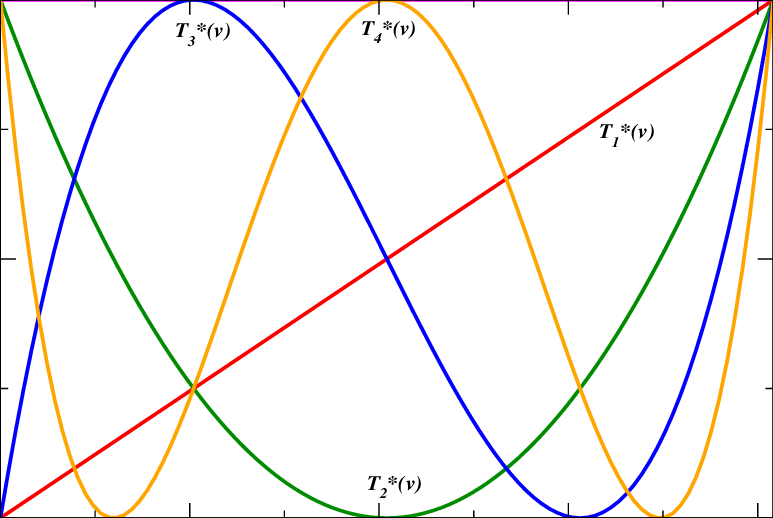
\includegraphics[scale=0.2]{images/cheb2.png}
    \caption{Chebyshev First 4 Polynomials }
    \label{fig:cp2}
\end{figure}


\textbf{Recommendations for Fitting Data}
\begin{enumerate}
    \item  Use the lowest order polynomial that gives a reasonable approximation to the data.  Do not over fit the data, or the fitted polynomial will follow every bit of the noise on the data.
    \item Realise that the fit may be bad near the ends of the data. 
    \item  Do not use the polynomial approximation outside the range of the input data. i.e. Do not extrapolate the data!
\end{enumerate}

\chapter{Results And Discussion}
Instead of using invariant mass of four leptons $m_{4l}$, histogram templates that were generated via simulation directly in the measurements, analytical shapes are considered that have the precedence of smoothing out the irregularities because of finite number of simulated events. For measuring $m_H$, or any other physics parameter for specific $m_H$ value, signal predictions as a function of $m_H$ are continuously parameterized first, based on the simulated MC samples values of that particular $m_H$ value.
\section{Signal Modelling Methodology}
\label{section:smm}
In order to take measurements in the on-shell region production of Higgs H(125), this analysis exploits the $105 < m_{4l} < 140$ GeV range, and is then parameterized in the range $118 < m_H <130$ GeV using five mass points of $m_H$ : 120, 124, 125, 126 and 130 GeV.
The probability density function (PDF) used to model the signal shapes
for different masses in every event category were explained earlier in section \ref{section:ec}.\\
To explain the signal PDF for $m_{4l}$ with an appropriate corresponding analytical function, one must consider both the experimental results and theoretical predictions. For small $m_H$ values, a narrow-width resonance hypothesis (that a relativistic Breit-Wigner function defines the theoretical signal line shape) holds. Also taken into account are the ECAL energy leakages, experimental resolution effects such as bremsstrahlung tails in the distributions and final state radiations.
The main reason for allocation of double-sided Crystal Ball (dCB) is that it takes in consideration; both the Gaussian resolution for the core region in $m_{4l}$ distribution, and also left right asymmetric end tails given by the power-law.
\subsection{Signal Line Shape}
A Double Crystal-Ball function $f_{dCB} (m_{4l} | m_H )$ as defined in \ref{section:dcb} is the fitting strategy used to deal with this situation, we have used the linear approximation of all the Double Crystal Ball parameters varying with $m_H$. All the six parameters ``$params$'' depend on $m_H$ and are calculated for each final state and event category.
\begin{equation}
    params = params_{CB0} + params_{CB1} \times (m_H - 125 GeV)
\end{equation}
In each final state, first $params_{CB0}$ parameters are gathered from the shapes using untagged category of $ggH$ production mode at $m_H$ = 125 GeV. The shape for every end state from this are shown in Fig.\ref{fig:smm}, which also illustrates that the resolution of muons is better than electrons. Subsequently, the $params_{CB1}$ parameters are calculated, a simultaneous fit is drawn for all other $m_H$ values. One should note, that we see no significant contrast between $ggH$ and $VBF$ signal shapes in rest of the categories. This is because they have very similar branching ratios when normalised but the parametrization done from production mode of $ggH$ for untagged event category is chosen for statistically limited cases.
\begin{figure}
    \centering
    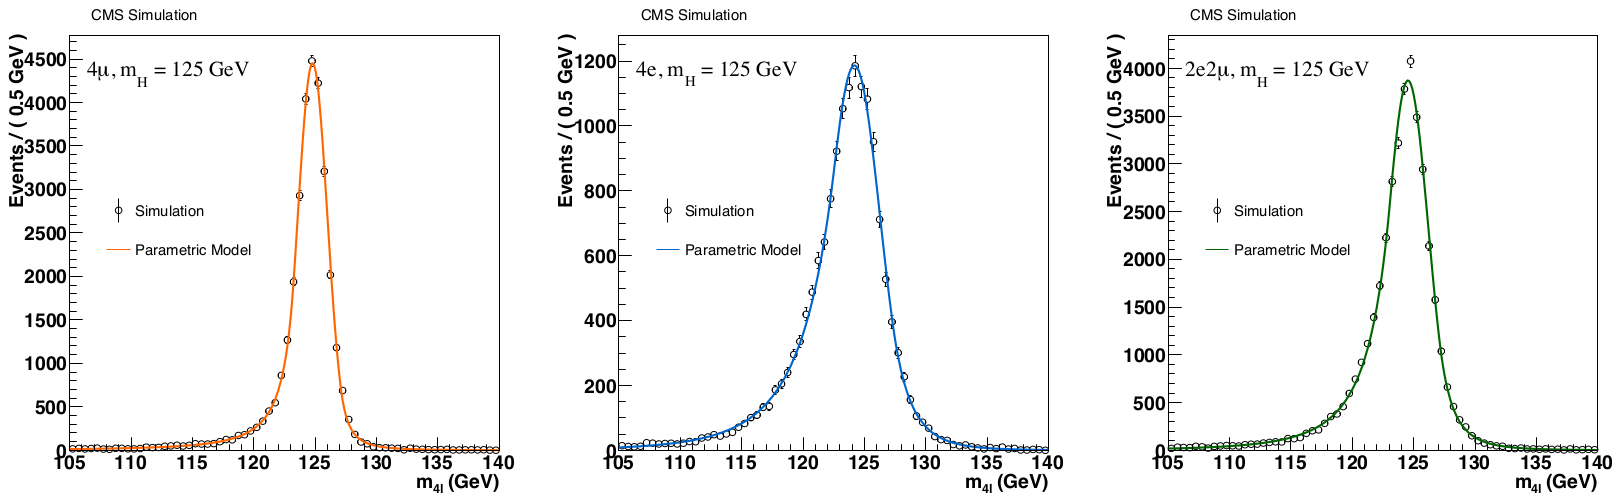
\includegraphics[scale=0.285]{images/sm.png}
    \caption{Probability density functions $f(m_{4l} |m_H)$ for ggH signal with $m_H$ =125 GeV after the full lepton and event selection. MC samples are fitted with the distributions defined in the text for $4\mu$ (left), 4e (center) and 2e2$\mu$ (right) events.}
    \label{fig:smm}
\end{figure}
In this way a unique PDF, extracted from the $ggH$ MC distribution, is valid for all the production mechanisms and categories. To check the quality of the
fits the Pull distributions as described in section \ref{section:pd} and ratio plots from Cauchy distribution described in section \ref{section:bwd} are also shown in Fig.\ref{fig:smm2}, showing an approximate Gaussian trend. The statement that pull distributions are expected to be standard Gaussian explained in section \ref{section:gd} implies a properly constructed parameterization for the simulated samples.\\
\begin{figure}[h]
    \centering
    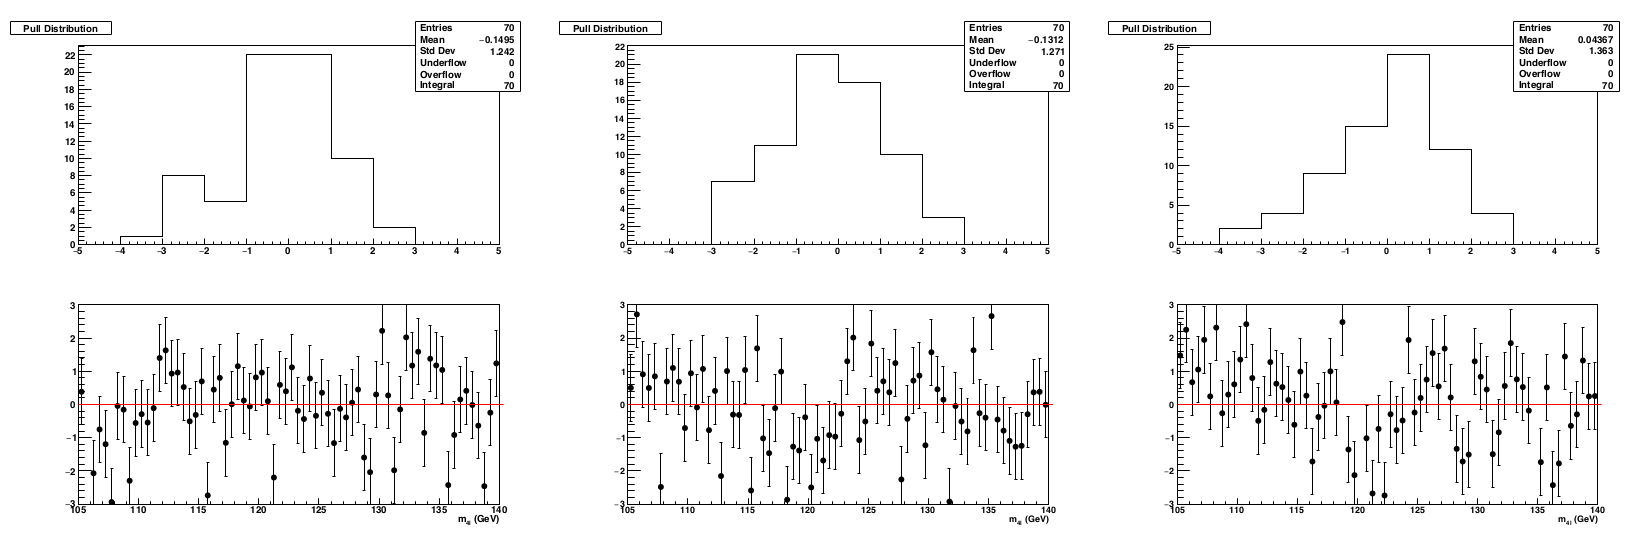
\includegraphics[scale=0.25]{images/sm2.png}
    \caption{Pull distribution (top) and the ratio distribution (bottom) for ggH signal with $m_H$ =130 GeV for 4$\mu$ (left), 4e (center) and 2e2$\mu$ (right) events.}
    \label{fig:smm2}
\end{figure}
For processes such as $WH, ZH,$ and $t\Paqt H$, the dislocated four leptons add a non-resonant component from interactions to the Higgs boson peak. A Landau function defined in section \ref{section:ld} is therefore included in the $dCB$ to perform the fit in the $m_H$ = 125 GeV case, which causes addition of two parameters, location parameter (which tells you where on the horizontal axis a graph is centered, relative to the standard normal model) and scale parameter (stretches or squeezes the graph), adjusted for simultaneous fitting. A normalization relative to each of both parameters is fixed for every category. Models fitted for all processes in each category using data of 2016, 2017 and 2018 are shown in Figure.\ref{fig:2016}, \ref{fig:2017} and \ref{fig:2018}.
\begin{figure}
    \centering
    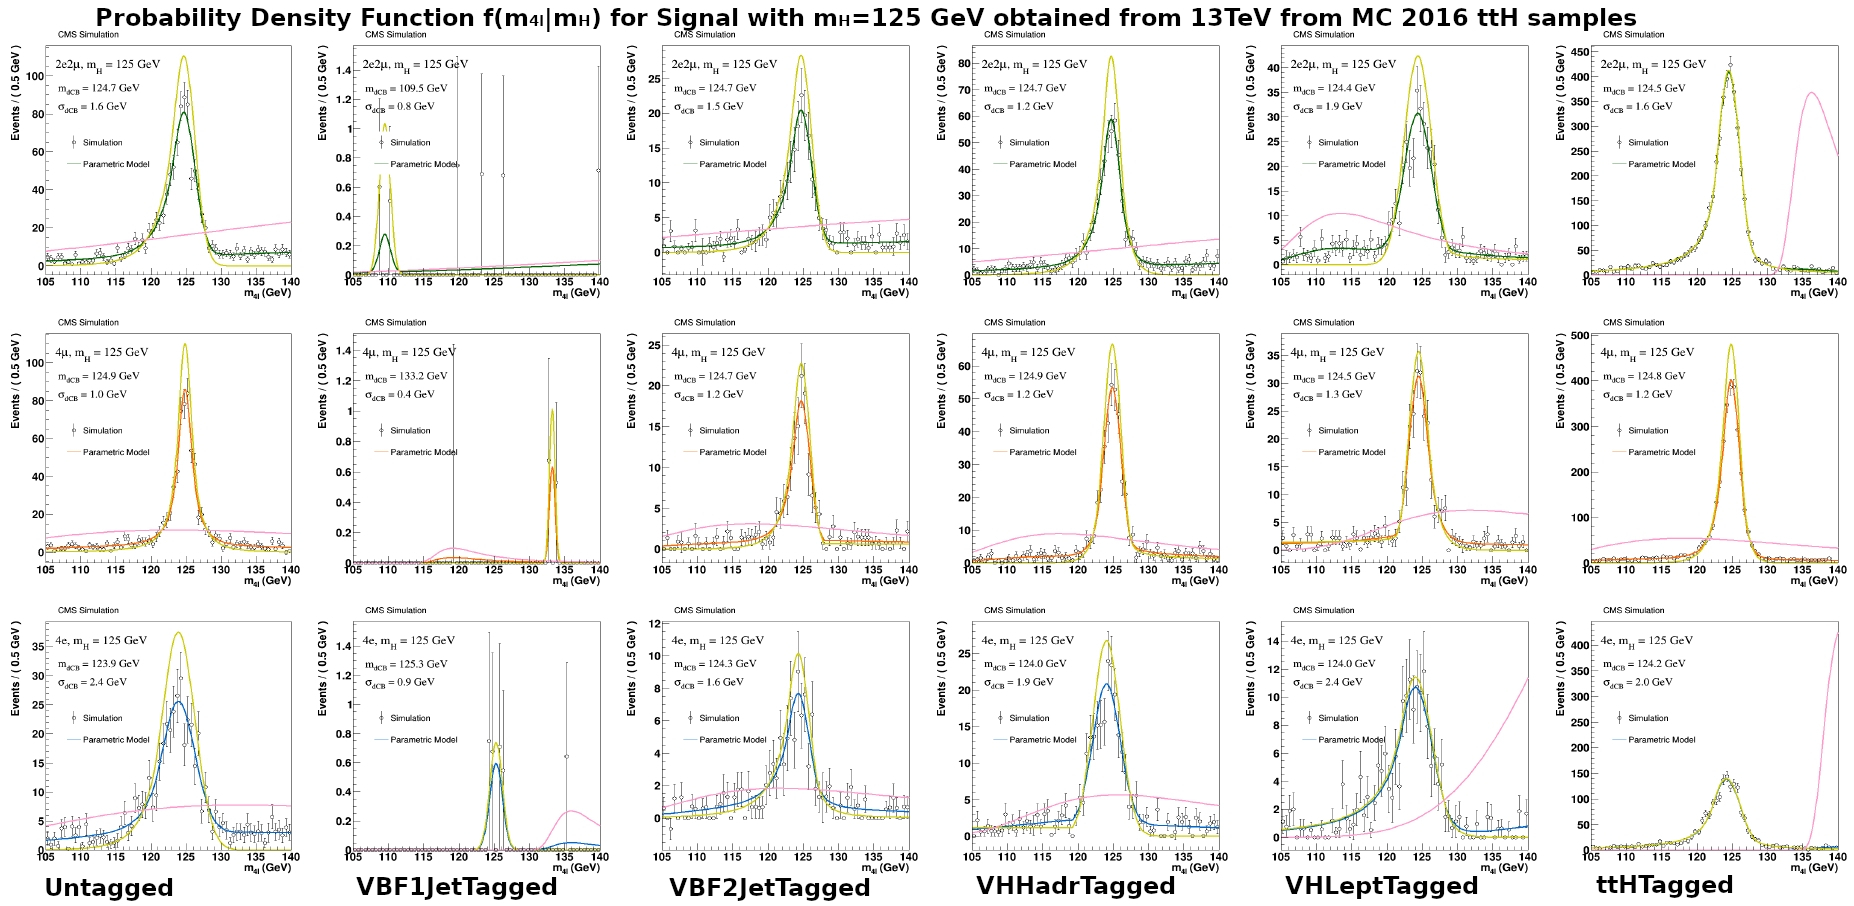
\includegraphics[scale=1]{images/2016.jpg} 
    \caption{Sum of probability density functions $f(m_{4l} |m_H)$ for $m_H$ =125 GeV fitted for 13TeV ttH 2016 MC samples.}
    \label{fig:2016}
\end{figure}
\begin{figure}
    \centering
    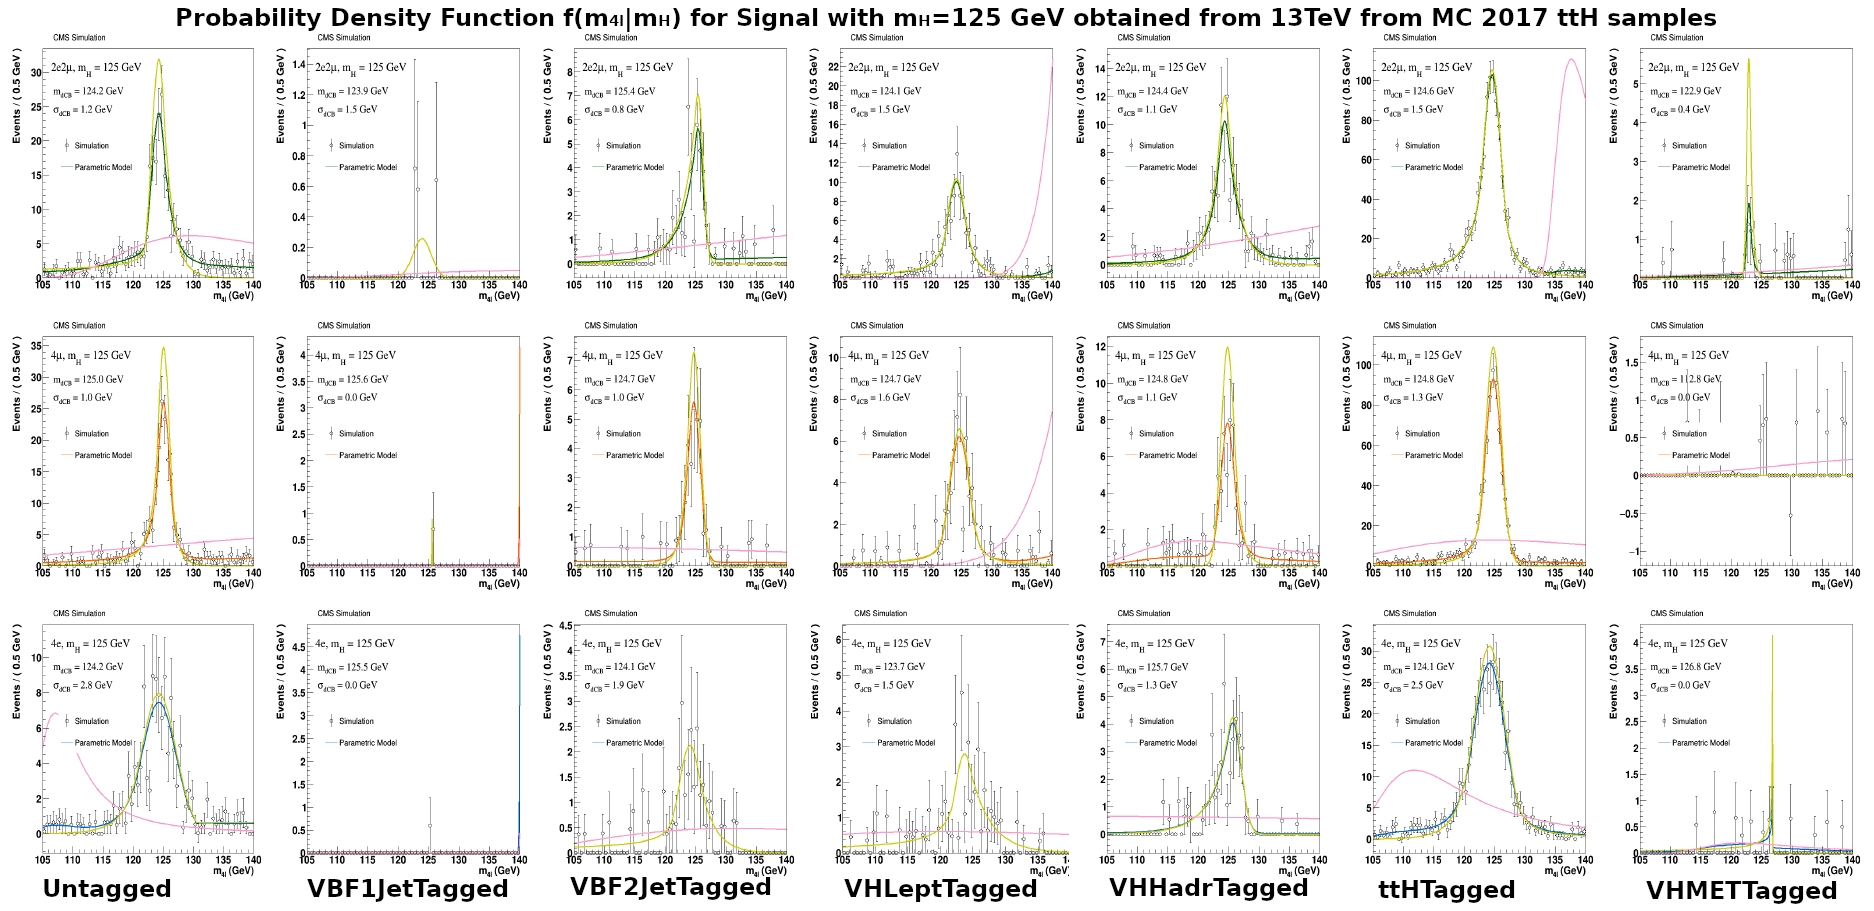
\includegraphics[scale=1]{images/2017.jpg}
    \caption{Sum of probability density functions $f(m_{4l} |m_H)$ for $m_H$ =125 GeV fitted for 13TeV ttH 2017 MC samples.}
    \label{fig:2017}
\end{figure}
\begin{figure}
    \centering
    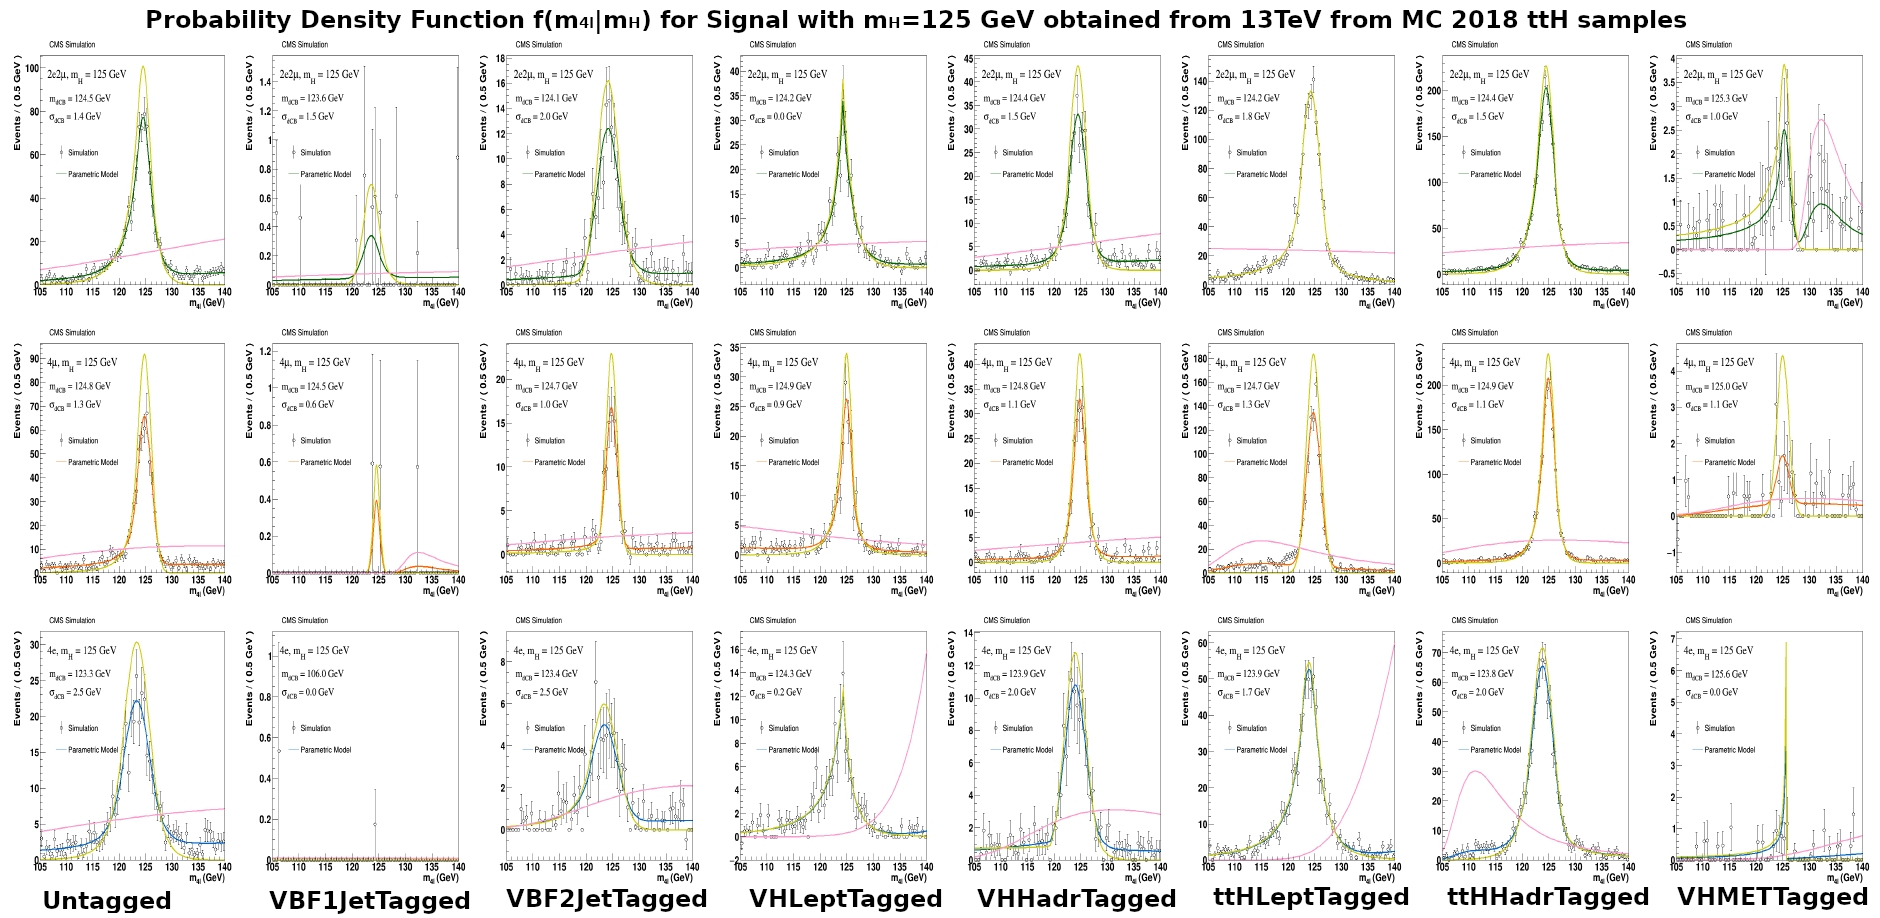
\includegraphics[scale=1]{images/2018.jpg}
    \caption{Sum of probability density functions $f(m_{4l} |m_H)$ for $m_H$ =125 GeV fitted for 13TeV ttH 2018 MC samples.}
    \label{fig:2018}
\end{figure}

\subsection{Signal Yield Parameterization}
The normalization of Higgs Boson signal in $dCB$, described in Eq.\ref{eqn:dcb}, is taken from simulation directly in the peak region. The parameterization of normalization constant N (for a given $m_H$) translates to estimated signal yields. Using simulated samples in $ 105 < m_{4l} < 140$ GeV signal window, for final states, all production modes and all event categories, a polynomial of second order is carried out for $m_H$ points (120, 124, 125, 126 and 130 GeV).\\
\begin{figure}[h]
     \centering
     \begin{subfigure}[b]{0.3\textwidth}
         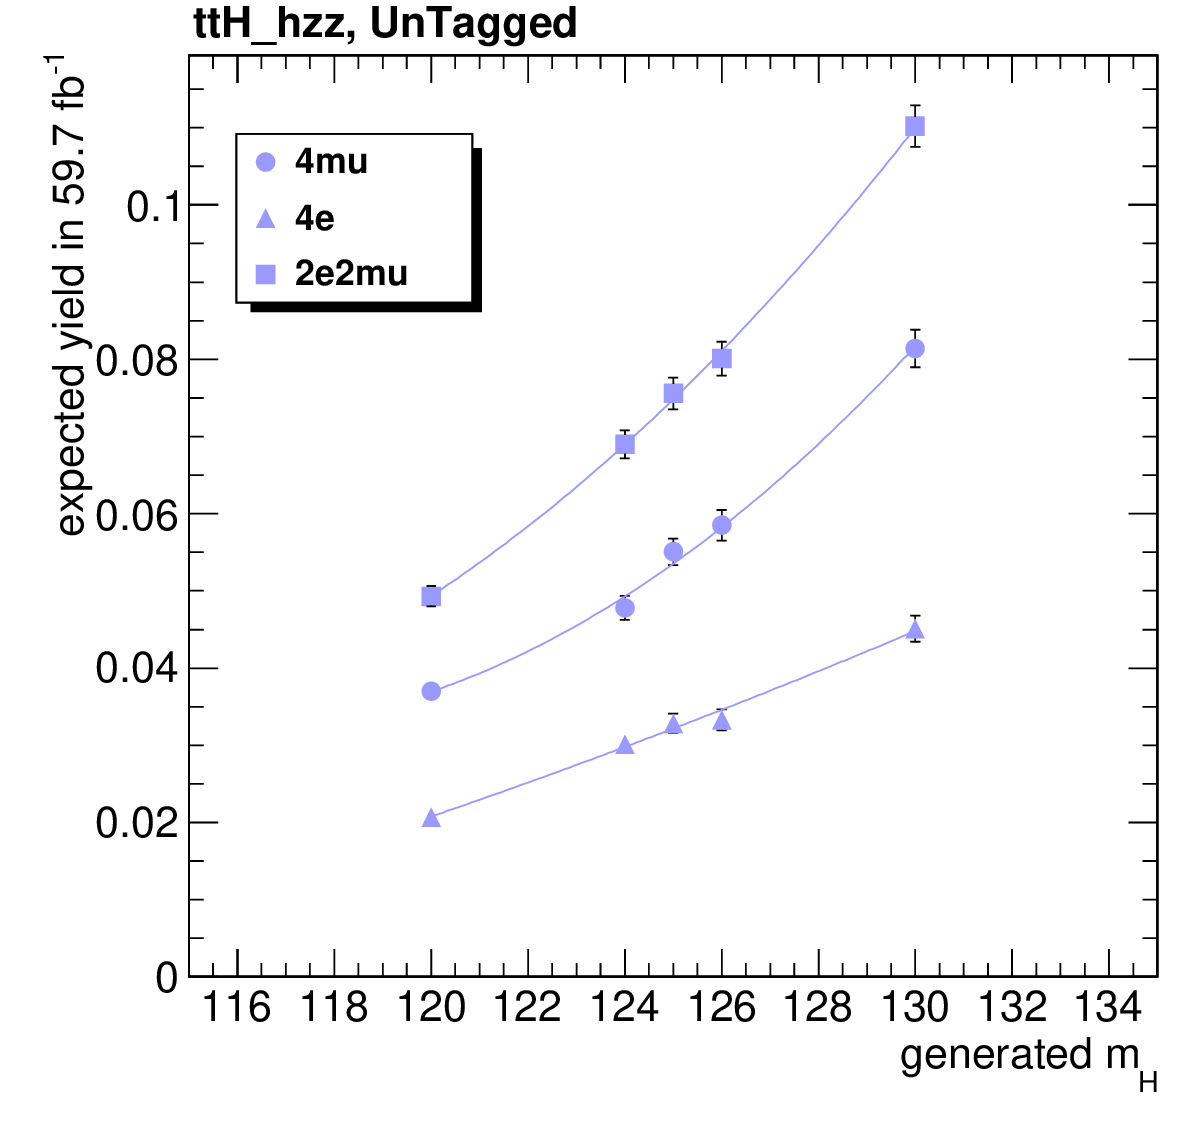
\includegraphics[width=\textwidth]{images/cFits_ttH_hzz_UnTagged_.png}
         \caption{UnTagged Category}
     \end{subfigure}
      \hfill
     \begin{subfigure}[b]{0.3\textwidth}
         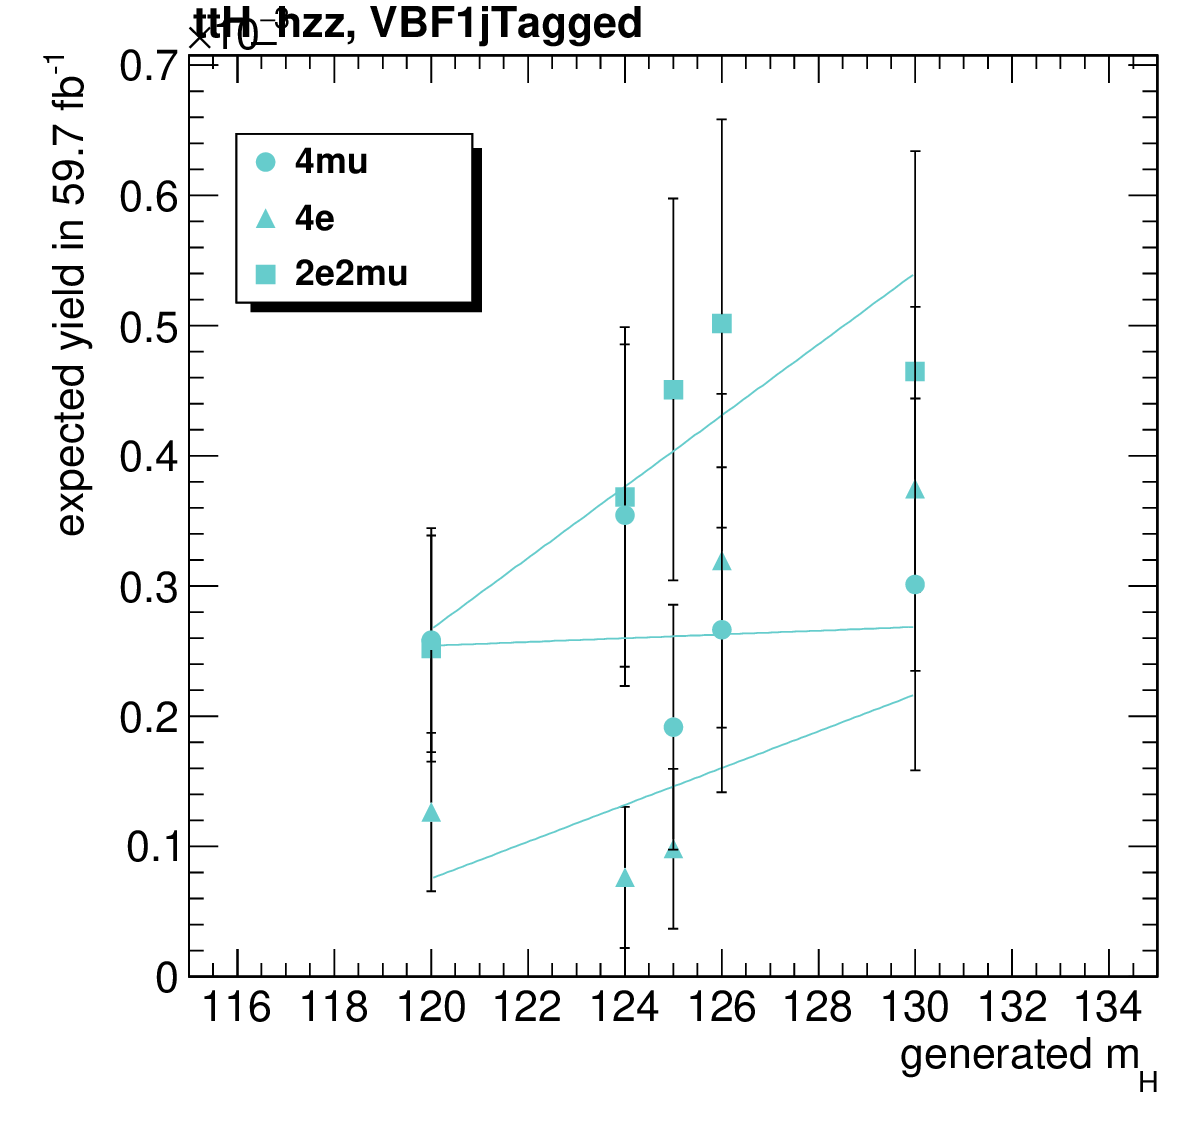
\includegraphics[width=\textwidth]{images/cFits_ttH_hzz_VBF1jTagged_.png}
         \caption{VBF1jTagged Category}
     \end{subfigure}
      \hfill
     \begin{subfigure}[b]{0.3\textwidth}
         
         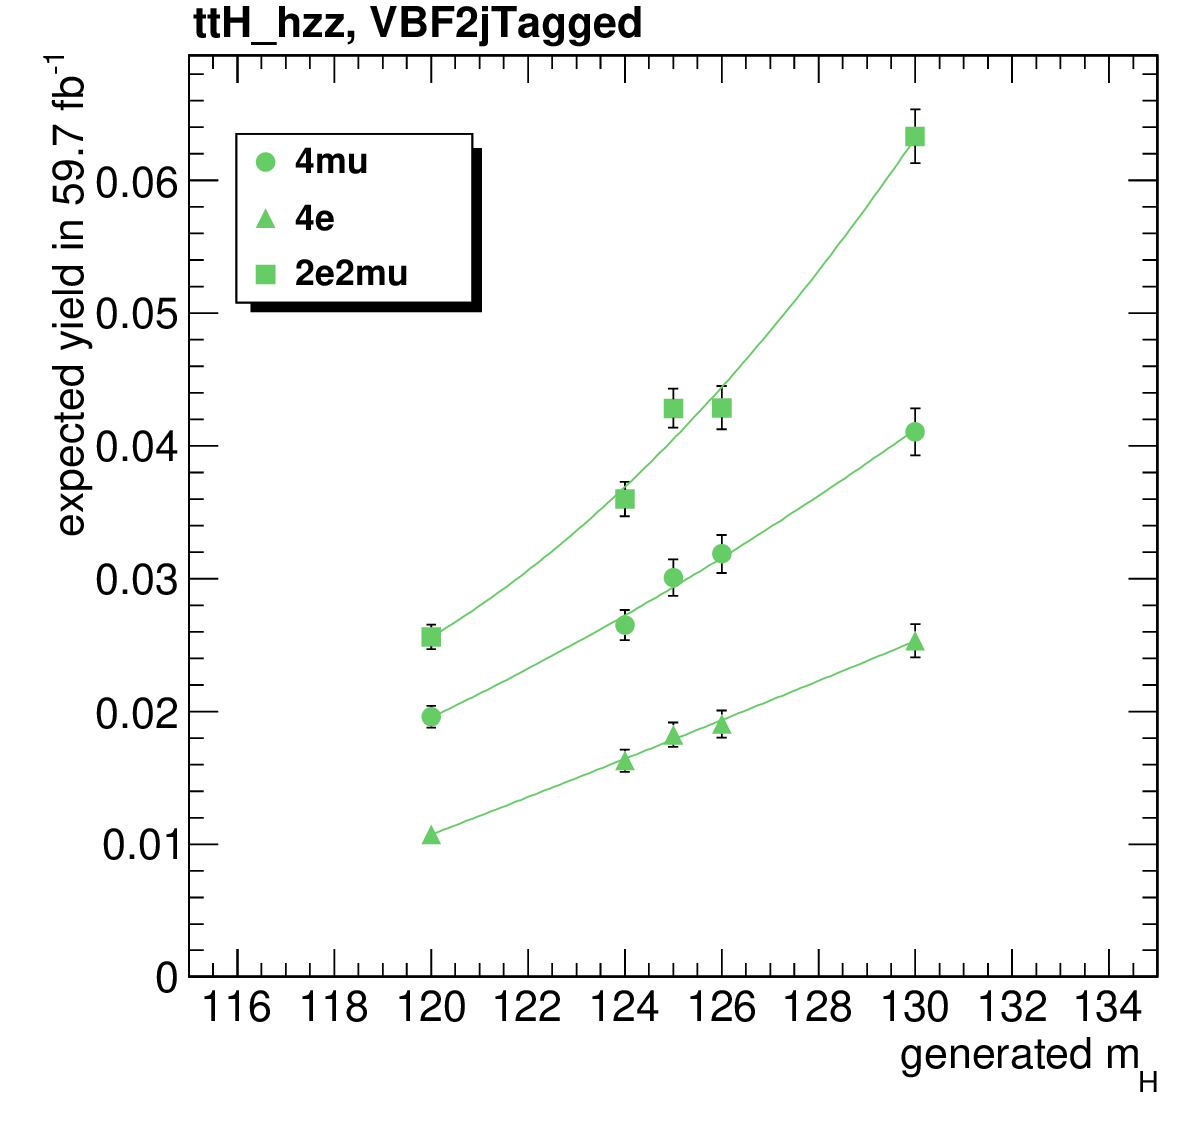
\includegraphics[width=\textwidth]{images/cFits_ttH_hzz_VBF2jTagged_.png}
         \caption{VBF2jTagged Category}
         \end{subfigure}
          \hfill
         \begin{subfigure}[b]{0.3\textwidth}
         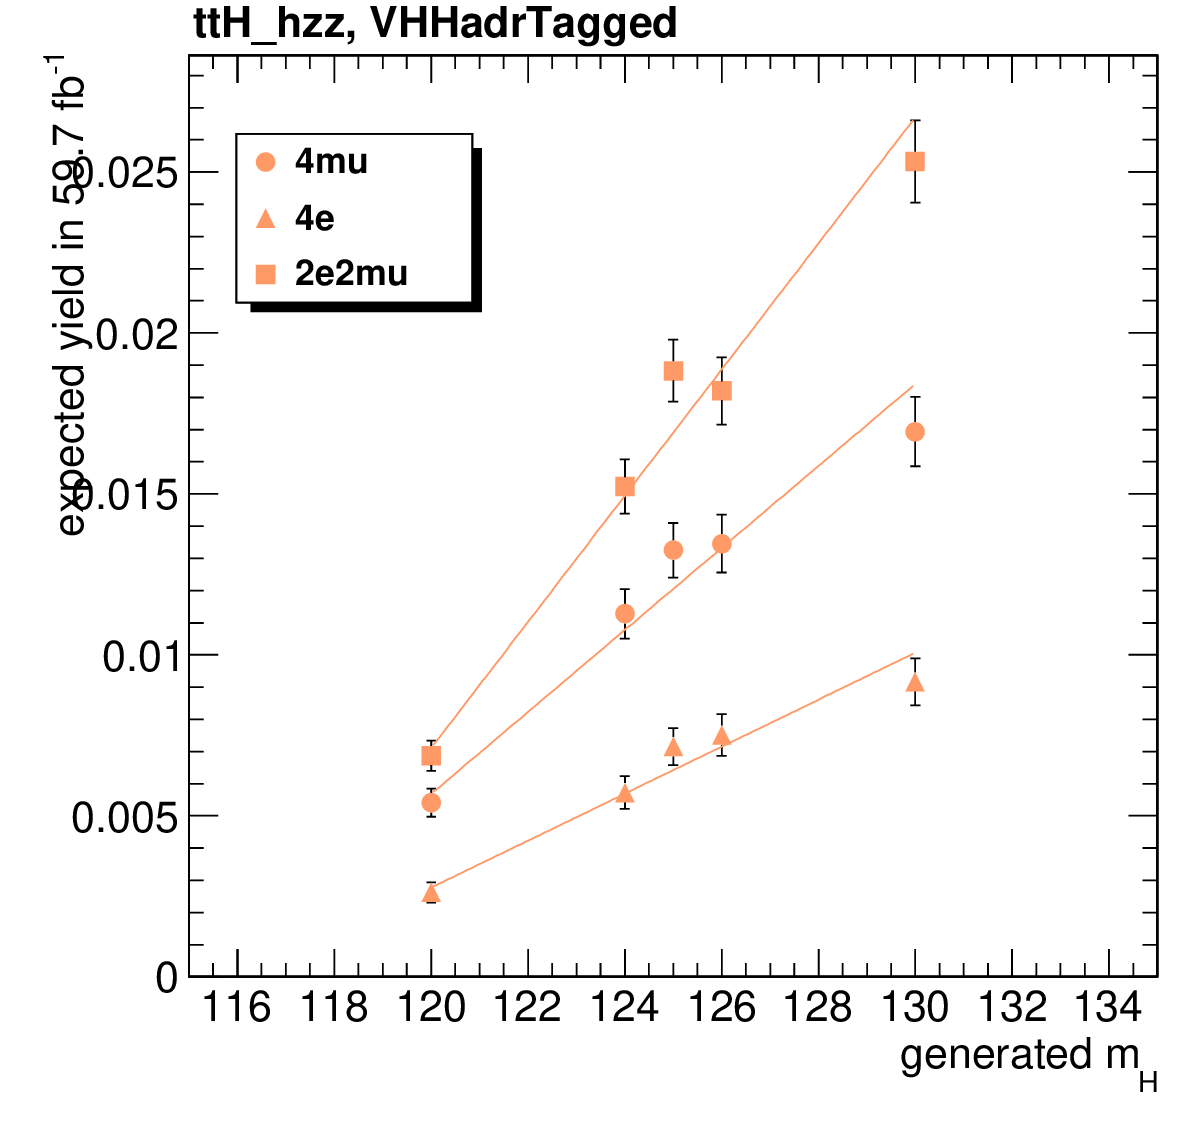
\includegraphics[width=\textwidth]{images/cFits_ttH_hzz_VHHadrTagged_.png}
         \caption{VHHadrTagged Category}
     \end{subfigure}
     \hfill
     \begin{subfigure}[b]{0.3\textwidth}
         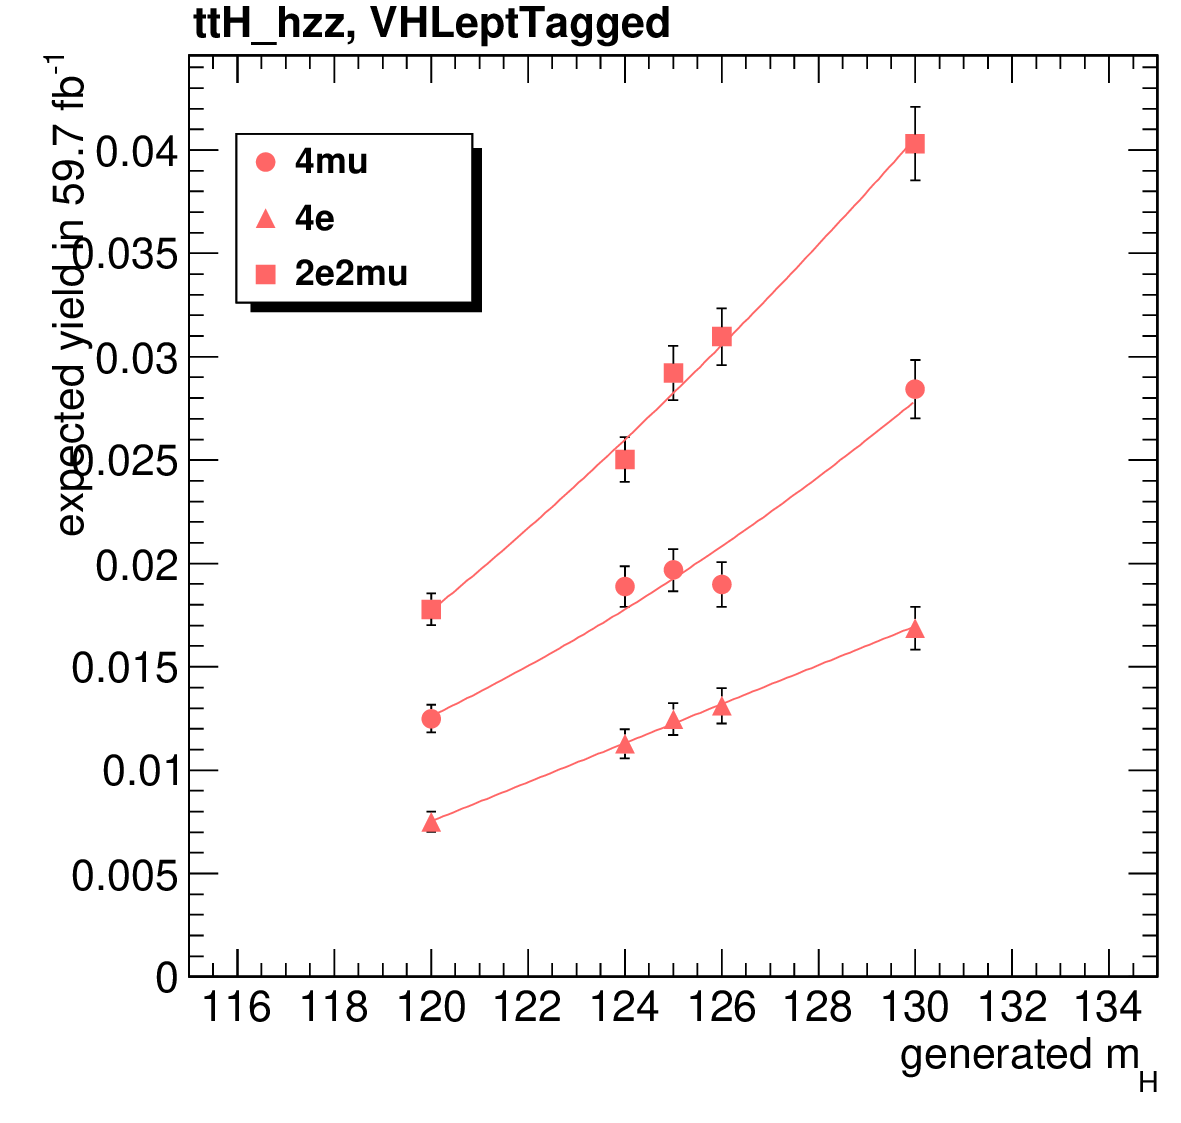
\includegraphics[width=\textwidth]{images/cFits_ttH_hzz_VHLeptTagged_.png}
         \caption{VHLeptTagged Category}
     \end{subfigure}
      \hfill
     \begin{subfigure}[b]{0.3\textwidth}
        
         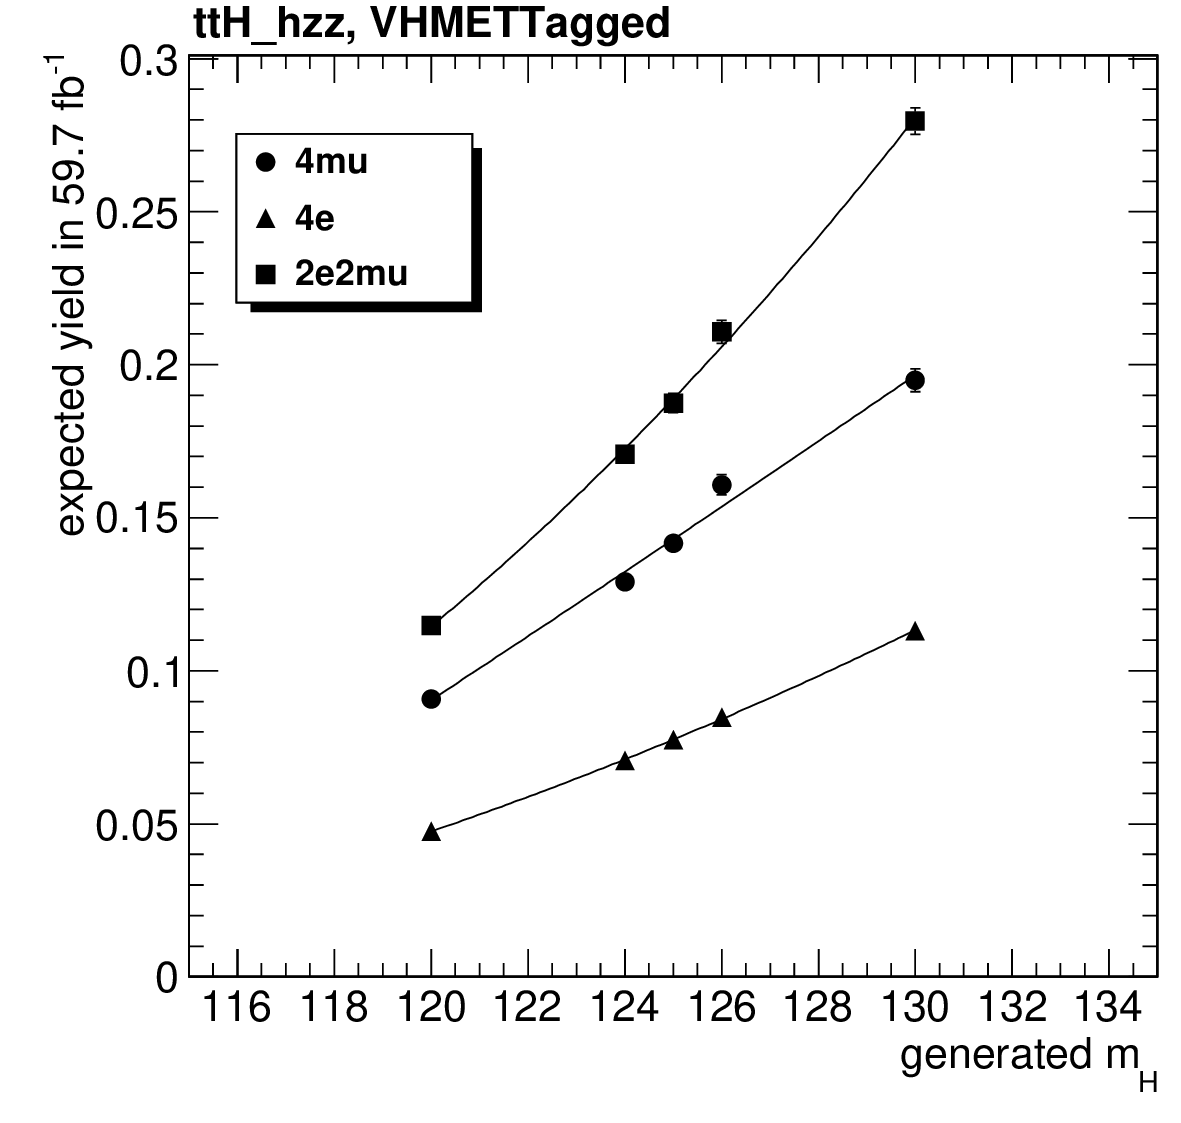
\includegraphics[width=\textwidth]{images/cFits_ttH_hzz_VHMETTagged_.png}
         \caption{VHMETTagged Category}
     \end{subfigure}
       \hfill
        \begin{subfigure}[b]{0.3\textwidth}
         
         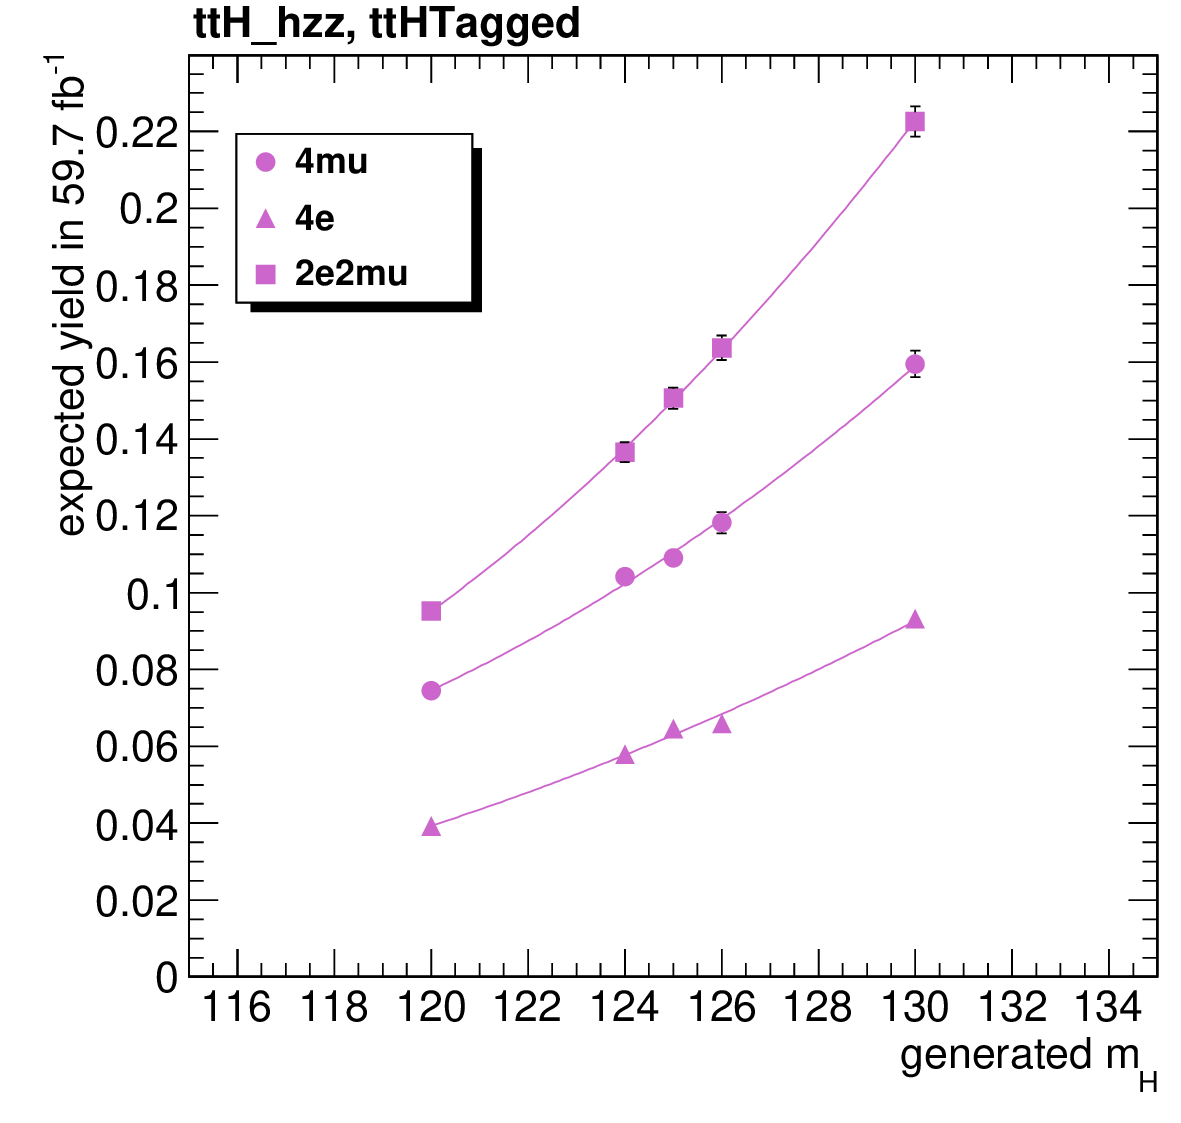
\includegraphics[width=\textwidth]{images/cFits_ttH_hzz_ttHTagged_.png}
         \caption{ttHTagged Category}
         \label{fig:five over x}
     \end{subfigure}
        \caption{Expected signal yields fits after full event
selection in a [105, 140] GeV $m_{4l}$ window, for the ttH production mode in the 2018 seven event category for an integrated luminosity of 59.7 fb$^{-1}$.}
        \label{fig:yield}
\end{figure}
A numerical analysis; spline interpolation, is used, which is a type of interpolation where interpolant is a form of piece-wise polynomial called a spline. It is given preference over polynomial interpolation as it can give similar results, with lesser degree polynomials.
Fits of the expected signal yields depended on $m_H$ for 59.7 $fb^{-1}$ in the $105 < m_{4l} < 140$ GeV range after fully selecting events, are parameterized in the range $118 < m_{4l} < 134$ GeV for 2018 MC data in Fig:\ref{fig:yield}.

\subsection{Signal Background Parameterization}
There are two kinds of background, the ``\textbf{reducible}'' backgrounds where particles fake the particles we are looking for (for example, a high energy electron can look just like a high energy photon) and the ``\textbf{irreducible}'' backgrounds where particles are the same kind as the ones we are looking for. 
\begin{itemize}
    \item \textbf{Irreducible} backgrounds which come from the production of $ZZ$ via quark anti-quark annihilation or gluon fusion, are estimated using simulation.
    \item  \textbf{Reducible} background is estimated using two independent methods having dedicated control regions in data.
\end{itemize}
During the study of $H \rightarrow Z Z^* \rightarrow 4l$, major irreducible backgrounds were from fusion of two gluons $gg \rightarrow ZZ$ and annihilation of quark anti-quark pair $q \bar{q} \rightarrow ZZ$ where $Z$ bosons decay into a lepton pair. In both cases, no intermediary Higgs boson is detected, Z boson pair is directly produced. The kinematics discriminant and expected yield are obtained from simulations by estimation of irreducible backgrounds.\\
\begin{figure}[h]
    \centering
    \begin{subfigure}[b]{0.8\textwidth}
     \includegraphics[width=\textwidth]{images/be.png}
     \caption{fusion of gluons $gg \rightarrow ZZ$}
     \label{fig:gg}
    \end{subfigure}
    \vfill
    \begin{subfigure}[b]{0.8\textwidth}
    \includegraphics[width=\textwidth]{images/be1.png}
    \caption{annihilation quark anti-quark $q \bar{q} \rightarrow ZZ$ }
     \label{fig:qq}
    \end{subfigure}
     \caption{Irreducible background fitting using Chebyshev's polynomials.}
    \label{fig:be}
\end{figure}
We have used third order Chebyshev's polynomials ``ChebPol'' explained in detail in section \ref{section:cp}. It is a multivariate interpolation, which contains methods for creating multivariate/multidimensional interpolations of functions on a hypercube. Examples for gluon fusion $gg \rightarrow ZZ$ in Fig.\ref{fig:gg} and quark antiquark annihilation $q \bar{q} \rightarrow ZZ$ in Fig.\ref{fig:qq} for 2018 data analysis in untagged category for 3 final states 4$\mu$, 4e and 2e2$\mu$ are illustrated as well as first three Chebyshev's polynomials with their pull distribution.\\
All categories for 2016, 2017 and 2018 data irreducible background is given in appendix \ref{appendix:be}.
\clearpage
\subsection{Results of Event Selection}
The events and their number observed in data with their yields for 35.9 fb$^{-1}$, 41.5 fb$^{-1}$ and 59.7 fb$^{ -1}$ of data collected in 2016,2017 and 2018 for Higgs signal and backgrounds after complete event reconstruction are reported in Table: \ref{tab:es6}, \ref{tab:es7} and \ref{tab:es8} for the full range of $m_{4l}$.
\begin{table}
    \centering
   \includegraphics[scale=0.4]{images/es6.png}
    \caption{Event's number for an integrated luminosity of 35.9 fb$^{-1}$.}
    \label{tab:es6}
\end{table}
\begin{table}
    \centering
   \includegraphics[scale=0.4]{images/es7.png}
    \caption{Event's number for an integrated luminosity of 41.5 fb$^{-1}$.}
    \label{tab:es7}
\end{table}
The estimated background and signal events numbers as well as observed candidates numbers are calculated after full event reconstruction, in every final state for mass range $m_{4l} >70$ GeV. Signal and ZZ background are calculated from MC simulation, while Z +X is calculated directly from data.\\
The error bars at every value are the so-called Garwood confidence intervals at 68$\%$ confidence level (CL) \cite{<fg>}. The expected distribution and observed distribution are in agreement within the statistical uncertainties over the whole spectrum.
\begin{table}
    \centering
   \includegraphics[scale=0.4]{images/es8.png}
    \caption{Event's number for an integrated luminosity of 59.7 fb$^{-1}$.}
    \label{tab:es8}
\end{table}

\section{Signal Strength Modifier Measurement}
The signal strength modifier $\mu$ is defined as the ratio of measured Higgs boson rate to the predicted theoretical Higgs boson rate in the SM, which categorizes Higgs boson yields. For a distinct production and decay mode $i \rightarrow H \rightarrow f$ the signal strength of production, $\mu_i$ is given by,
\begin{equation}
    \mu_i = \frac{\sigma_i}{(\sigma_i)_{SM}}, \hspace{5mm} and  \hspace{5mm}  \mu^f = \frac{B^f}{(B^f)_{SM}}
\end{equation}
Here, $\sigma_i$ ($i$=ggH,VBF,WH,ZH,t$\bar{t}$H) are production cross sections for $i \rightarrow H$ and $B^f$ ($f=ZZ$) as we consider only the golden channel, is the decay branching ratio $H \rightarrow f$. The subscript SM represents the corresponding predicted SM values, which are $\mu_i$=1 and $\mu^f$=1. The product of $\mu_i$ and $\mu^f$ can be experimentally measured, leading to signal strength $\mu^f_i$ for combined production and decay;
\begin{equation}
    \mu^f_i = \frac{\sigma_i . B^f }{(\sigma_i)_{SM} . (B^f)_{SM}} = \mu_i . \mu^f
\end{equation}
To exploit all the properties of the resonance under study or search, a multi-dimensional fit is implemented. For every category described in
section \ref{section:ec}, two variables are taken in consideration for the maximum likelihood fit, namely:
\begin{enumerate}
    \item The four-lepton mass $m_{4l}$,
    \item The kinematic discriminant $D^{kin}_{bkg}$.
\end{enumerate}
To account for the strong correlation of the kinematic discriminant with
the mass, a 2D histogram template of $D^{kin}_{bkg}$ vs. $m_{4l}$ is implemented. Due to the small number of expected events in the mass peak, the unbinned data (fitted data except goodness of fit) is used for mass dimension and the resolution model is used as described in section \ref{section:smm}. The total PDF is defined as:
\begin{equation}
    \mathcal{L}_{2D} (m_{4l}) = \mathcal{L} (m_{4l}) \mathcal{L} (D^{kin}_{bkg} | m_{4l})
    \label{eqn:mdf}
\end{equation}
where the first factor corresponds to the 1D mass PDF and the second factor
to the 2D template of mass vs. kinematic discriminant. The conditional term
in the second factor is implemented in the template by normalizing all $D^{kin}_{bkg}$ columns corresponding to the same mass value each. Therefore, the 2D template does not include any information on the mass, but given the mass, it provides information on the kinematic discriminant.\\
In this section, we describe the method used for estimation of the signal strength, i.e. its total cross section normalized to the one expected for a SM Higgs. A multi-dimensional fit is implemented as explained by the Eq.\ref{eqn:mdf}.
These results are compatible with SM expectations under the uncertainties, which in our current events are majorly statistical. The results are compared to the expected signal-strength modifiers in Table.\ref{tab:tab2018}.
\begin{table}[]
    \centering
    \includegraphics[width=\textwidth]{images/tab2016.png}
    \caption{Expected and observed signal strength modifier at 35.9 fb$^{-1}$.}
    \label{tab:tab2016}
\end{table}
\begin{table}[]
    \centering
    \includegraphics[width=\textwidth]{images/tabcomb.png}
    \caption{Expected and observed signal strength modifier at 77.4 fb$^{-1}$.}
    \label{tab:comb}
\end{table}
\begin{table}
\centering
\includegraphics[scale=0.3]{images/tab2018.png}
\caption{Expected and observed signal strength modifier at 137.1 $^{-1}$. \cite{<colab2>}}
\label{tab:tab2018}
\end{table}
Two signal-strength modifiers for the five main Higgs production modes are calculated as scale factors for vector boson and fermionic contribution to the expected SM cross section. A two-dimensional fit is executed by the CMS collabortion \cite{<colab1>,<colab2>}, fixing the mass to $m_H = 125.38 GeV$ and profiling the likelihood for all nuisance parameters, leading to the results illustrated in the top row of Fig.\ref{fig:mss}, where $\mu_{WH}$ and $\mu_{ZH}$ are split into leptonically decaying bosons $\mu_{WHlep}$ /$\mu_{ZHlep}$ and hadronically decaying bosons
$\mu_{WHhadr}$ /$\mu_{ZHhadr}$. Also the $\mu_{ttH}$ splits into leptonically decaying fermions $\mu_{ttHlept}$ and hadronically decaying fermions $\mu_{ttHhadr}$. The 68$\%$ and 95$\%$ CL contours in the ($\mu_{ggH,ttH,bbH,qtH}, \mu_{VBF,VH}$) plane are shown in bottom row of Fig.\ref{fig:mss}.
\begin{figure}[h]
     \centering
     \begin{subfigure}[b]{0.3\textwidth}
         \includegraphics[width=\textwidth]{images/ssm2016.png}
         \caption{2016 observed values}
     \end{subfigure}
      \hfill
     \begin{subfigure}[b]{0.3\textwidth}
         \includegraphics[width=\textwidth]{images/2017ssm.png}
         \caption{2017 observed values}
     \end{subfigure}
      \hfill
     \begin{subfigure}[b]{0.3\textwidth}
         
         \includegraphics[width=\textwidth]{images/ssm2018.png}
         \caption{2018 observed values}
         \end{subfigure}
          \hfill
         \begin{subfigure}[b]{0.3\textwidth}
         \includegraphics[width=\textwidth]{images/ssm2016b.png}
         \caption{2016 2D likelihood}
     \end{subfigure}
     \hfill
     \begin{subfigure}[b]{0.3\textwidth}
         \includegraphics[width=\textwidth]{images/2017ssmb.png}
         \caption{2017 2D likelihood}
     \end{subfigure}
      \hfill
     \begin{subfigure}[b]{0.3\textwidth}
        
         \includegraphics[width=\textwidth]{images/ssm2018b.png}
         \caption{2018 2D likelihood}
     \end{subfigure}
        \caption{Observed values, in each event category, of the signal strength $\mu = \sigma / \sigma_{SM}$, where the vertical line shows combined $\mu$. $\pm 1\sigma$ uncertainties can be seen as filled band along horizontal bars (top row). A likelihood in 2D space for the $\mu_{fermionic}$ and $\mu_{bosonic}$. The dashed and solid contours illustrate 68$\%$ and 95$\%$ CL regions, respectively. The diamond shows the expected values for the SM Higgs boson where as the cross points to the best-fit values (bottom row). \cite{<colab1>,<colab2>}}
        \label{fig:mss}
\end{figure}

\chapter*{Conclusion}
\vspace{-8mm}
\hspace{5mm} In this thesis, the Higgs signal from the $H \rightarrow ZZ \rightarrow 4l$ is studied for the data collected in 2016, 2017 and 2018 corresponding to integrated luminosity 35.9 fb$^{-1}$, 41.5 fb$^{-1}$ and 59.7 fb$^-1$ respectively, during in Run II of LHC by the CMS experiment at the centre of mass energy 13 TeV.\\

The analysis techniques are enhanced by targeting sub-dominant production modes and new event categories are introduced every year; in 2017 associated VH and associated $t\bar{t}H$ production modes are selected for hardonic and leptonic decay channels. In 2018 the categories; Untagged, VBF-2jet, VH-hadronic, and VH-leptonic are subdivided utilizing new variables like ZZ candidate transverse momentum and the two jets with leading invariant masses.\\

The Higgs boson signal is modelled using Double Sided Crystal Ball function $dCB$ around Higgs mass $m_H = 125$ GeV. The sum of PDF are fitted for all production modes using Run II MC samples. The irreducible background for fusion of two gluons $gg \rightarrow ZZ$ and annihilation of quark anti-quark $q\bar{q} \rightarrow ZZ$ is fitted using the Chebyshev's polynomial estimation for third order. A pull distribution is also graphically shown to validate the statistical functions used.\\

The properties, such as signal strength are measured in four lepton channel by the dectector. The expected value of signal strength is $\mu_{expected} = 1.00^{+0.08}_{-0.07}$(stat)$^{+0.10}_{-0.08}$(syst) and the observed value is $\mu_{observed} = 0.94\pm0.07$(stat)$^{+0.09}_{-0.08}$(syst). So far the measurement performed shows consistency in the properties of the Higgs, inside the current precision, compared to SM expectations with a minimal scalar sector, such as one physical Higgs boson used.\\

The HL-LHC is going open pathways for Higgs study, producing around $1.7 \times 10^8$ Higgs and $\PHiggs \PHiggs$ events upto $1.21 \times 10^5$ with an integrated luminosity of 3000 fb$^{-1}$ at $\sqrt{s}$ = 14 TeV. Run III of LHC will further the study of rare decays of SM Higgs and its properties, Higgs couplings, pair production in Higgs, and new physics in Higgs sector in Beyond Standard Model (BSM), Dark Matter-Higgs coupling, or if it is composite (a Goldstone boson).


\bibliographystyle{unsrt}
\bibliography{references}

\appendix
\chapter{Irreducible Background}
\label{appendix:be}
\section{Background Estimation For of Run II}
\subsection{Fit of Gluon Fusion Background}

\begin{figure}[h]
    \centering
    \includegraphics[scale=0.6]{images/2016gg.jpg}\\
    \text{(a) $gg \rightarrow ZZ$ 2016 Data.}
     \vspace*{-15mm}
\end{figure}

\begin{figure}[h]
 \vspace*{-15mm}
 \centering
\begin{subfigure}[b]{0.8\textwidth}
    \includegraphics[scale=0.6]{images/2017gg.jpg}
    \caption{$gg \rightarrow ZZ$ 2017 Data.}
\end{subfigure}
\vfill
\begin{subfigure}[b]{0.8\textwidth}
    \includegraphics[scale=0.6]{images/2018gg.jpg}
    \caption{$gg \rightarrow ZZ$ 2018 Data.}
\end{subfigure}
\caption{Gluon Fusion}
\end{figure}
\clearpage
\subsection{Fit of Quark Anti-Quark Background}

\begin{figure}[h]
\vspace*{-8mm}
    \centering
    \begin{subfigure}[b]{0.75\textwidth}
    \includegraphics[scale=0.6]{images/2016qq.jpg}
    \caption{$q \bar{q} \rightarrow ZZ$ 2016 Data.}
\end{subfigure}
\vfill
\begin{subfigure}[b]{0.75\textwidth}
    \includegraphics[scale=0.6]{images/2017qq.jpg}
    \caption{$q \bar{q} \rightarrow ZZ$ 2017 Data.}
\end{subfigure}
\vfill
\begin{subfigure}[b]{0.75\textwidth}
    \includegraphics[scale=0.6]{images/2018qq.jpg}
    \caption{$q \bar{q} \rightarrow ZZ$ 2018 Data.}
\end{subfigure}
\caption{Quark Anti-Quark Annihilation}
\vspace*{-5mm}
\end{figure}
\end{document}
